\subsection{Kinect with rotations motion at 10 cm/s}

The figures in this section show the detailed results of test performed with the Kinect sensor with a 20 mm resolution map in the flying arena performing several rotations in the air and moving at 10 cm/s.


%Animated paths
\begin{figure}[H]
	\centering
	\animategraphics[width=0.75\textwidth,loop,autoplay,controls]{1}{appendices/tests-6dof/kinect/\currfilebase/images-drl/image}{1}{60}
	\caption{Point clouds projected on top of the map using the localization system poses}
	\label{fig:localization-system-evaluation_kinect_rotations}
\end{figure}

\begin{figure}[H]
	\centering
	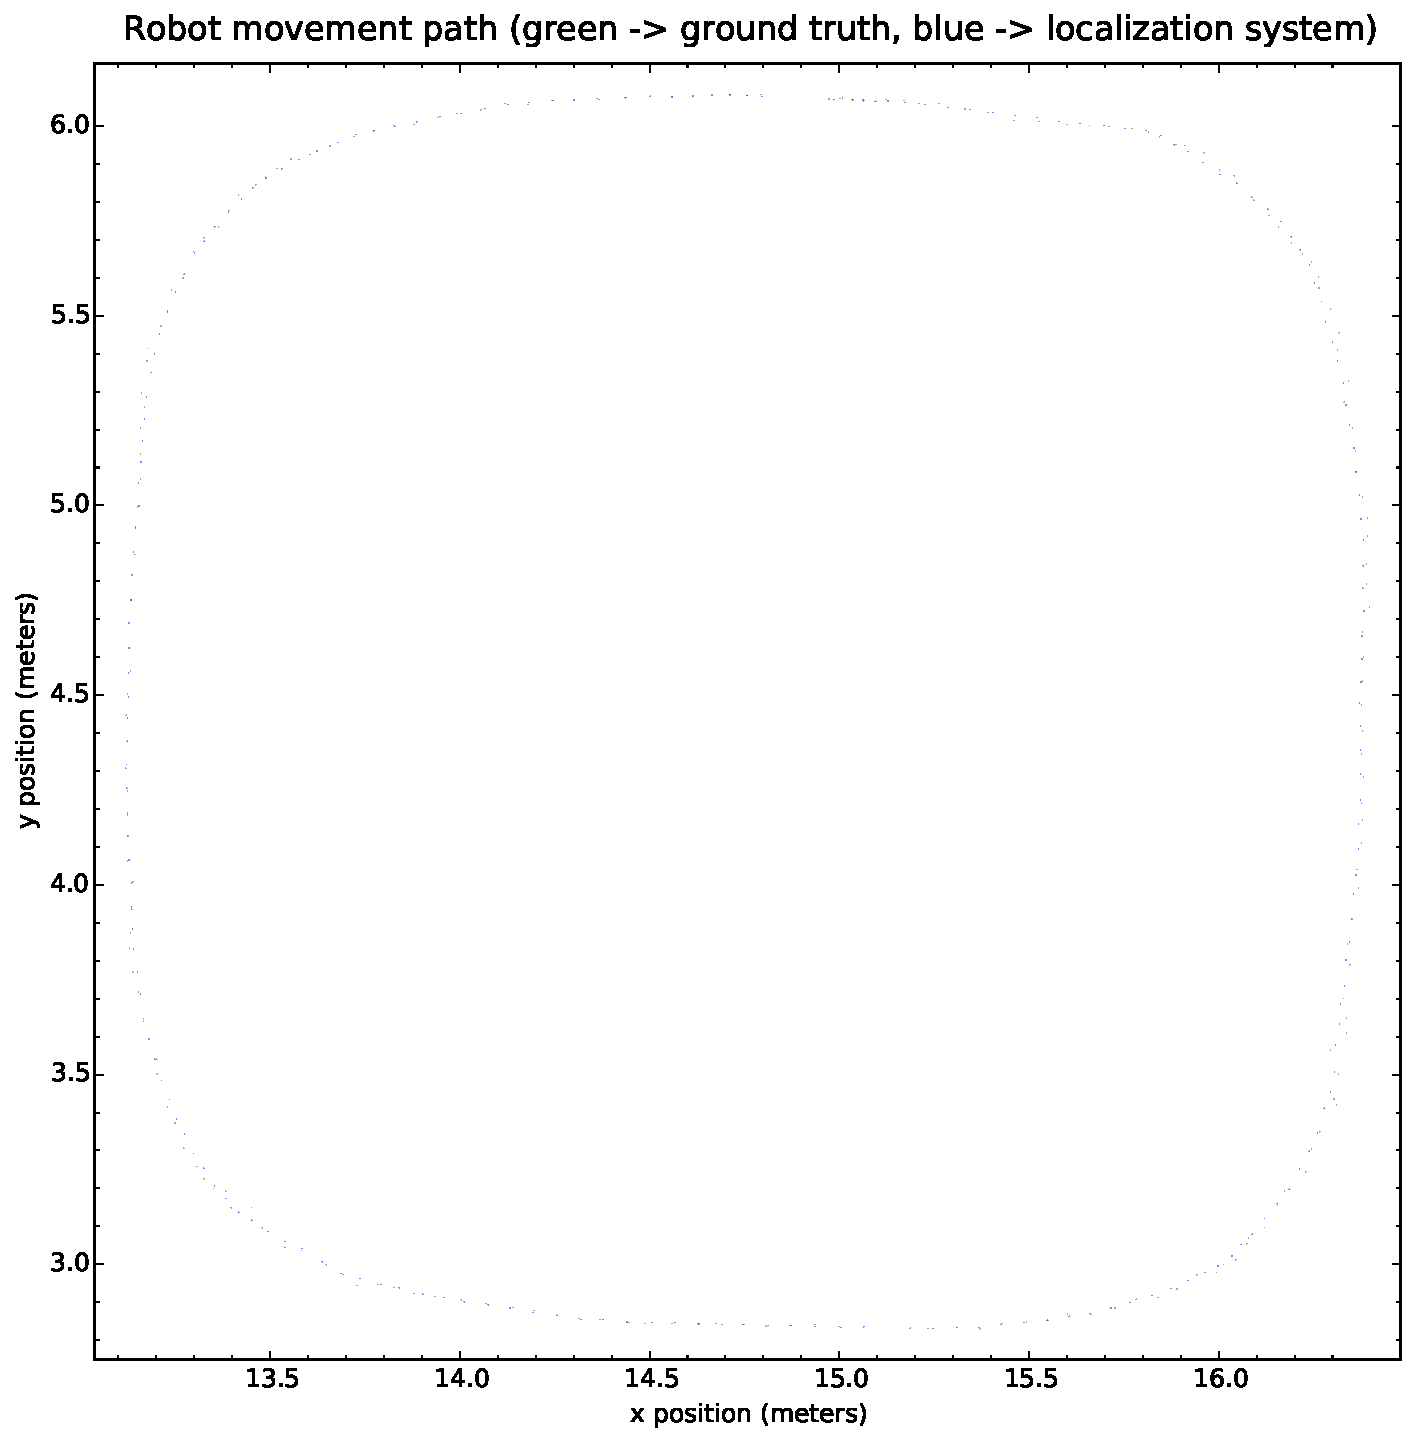
\includegraphics[width=0.75\textwidth]{appendices/tests-6dof/kinect/\currfilebase/graphs/robot-movement-path}
	\caption{Poses estimated by the ground truth and localization system}
\end{figure}


%Point cloud assembly
\begin{figure}[H]
	\centering
	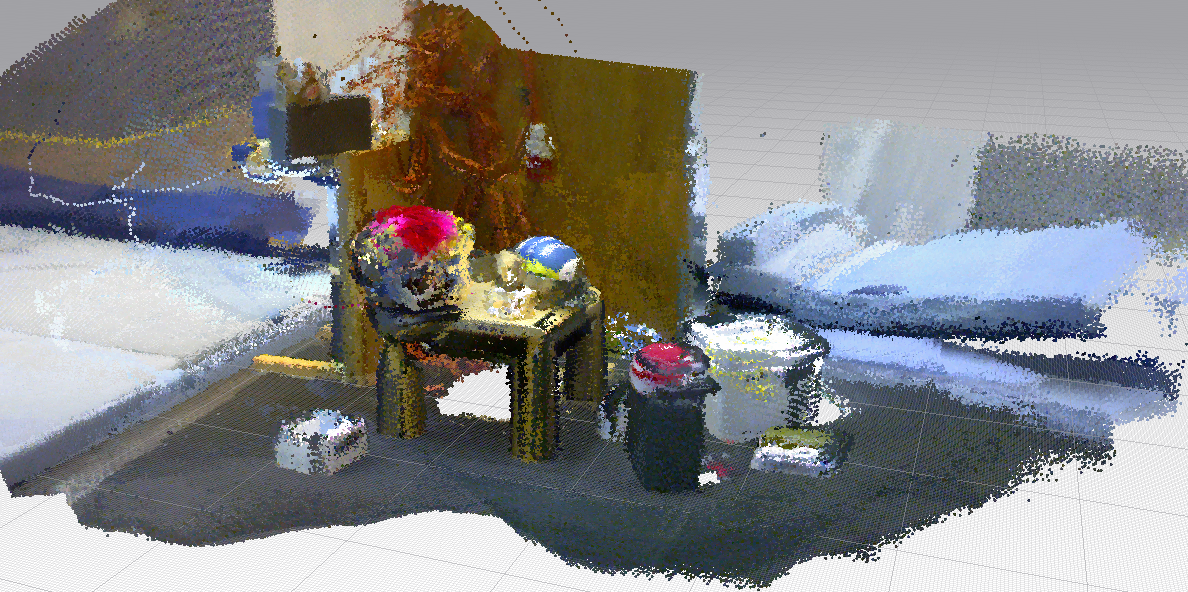
\includegraphics[width=0.99\textwidth]{appendices/tests-6dof/kinect/\currfilebase/ground-truth-cumulative}
	\caption{Point clouds assembled on top of the map using the ground truth poses}
\end{figure}

\begin{figure}[H]
	\centering
	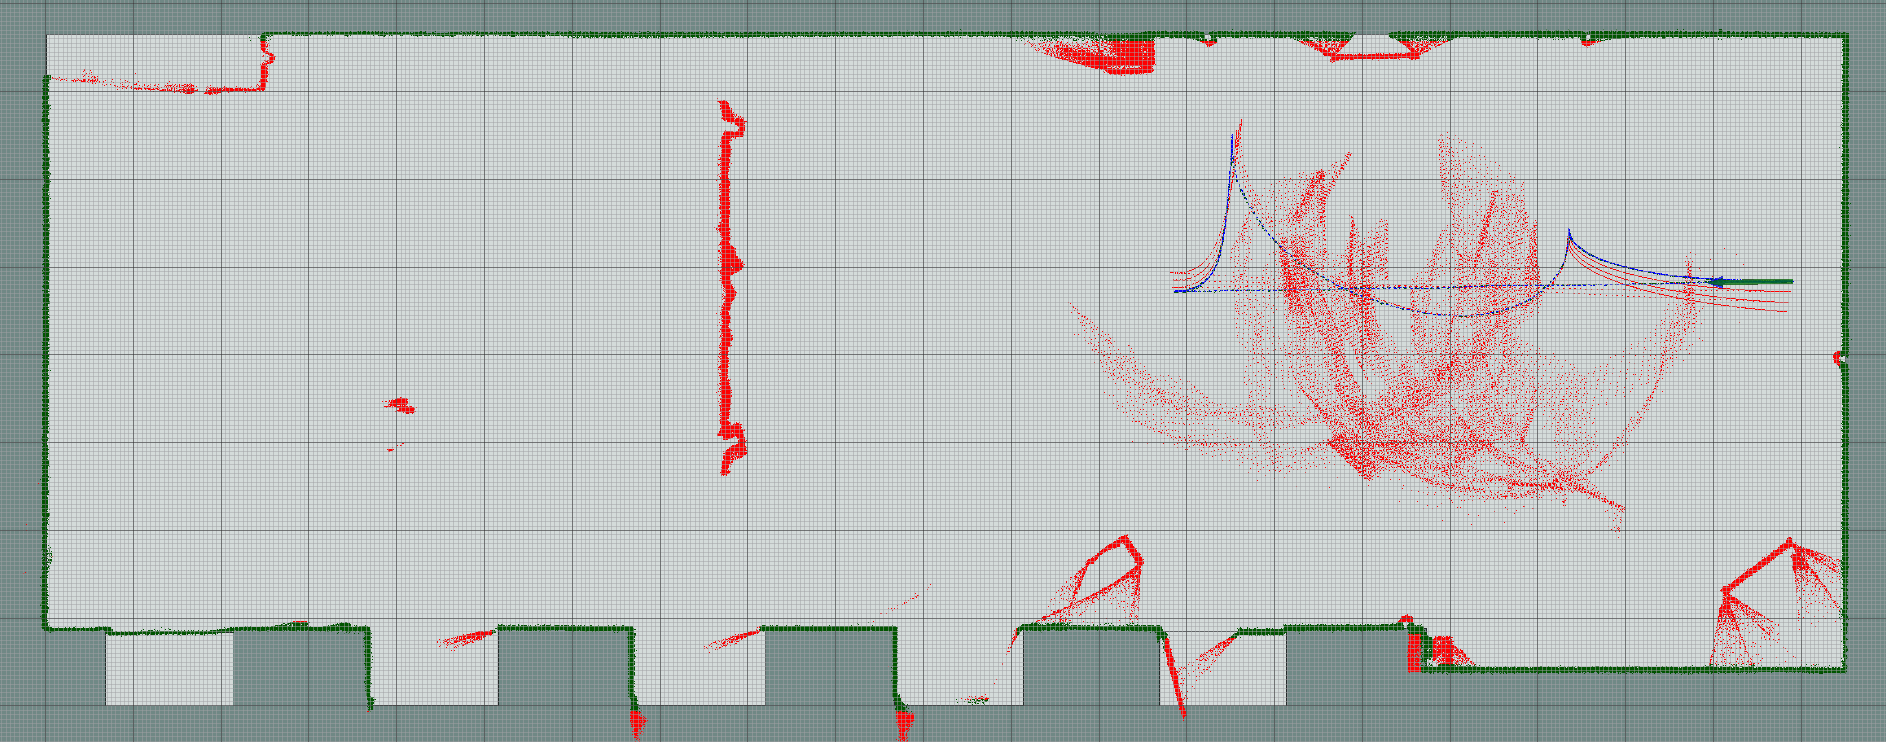
\includegraphics[width=0.99\textwidth]{appendices/tests-6dof/kinect/\currfilebase/drl-cumulative}
	\caption{Point clouds assembled on top of the map using the localization system poses}
\end{figure}


%Paths
\begin{figure}[H]
	\centering
	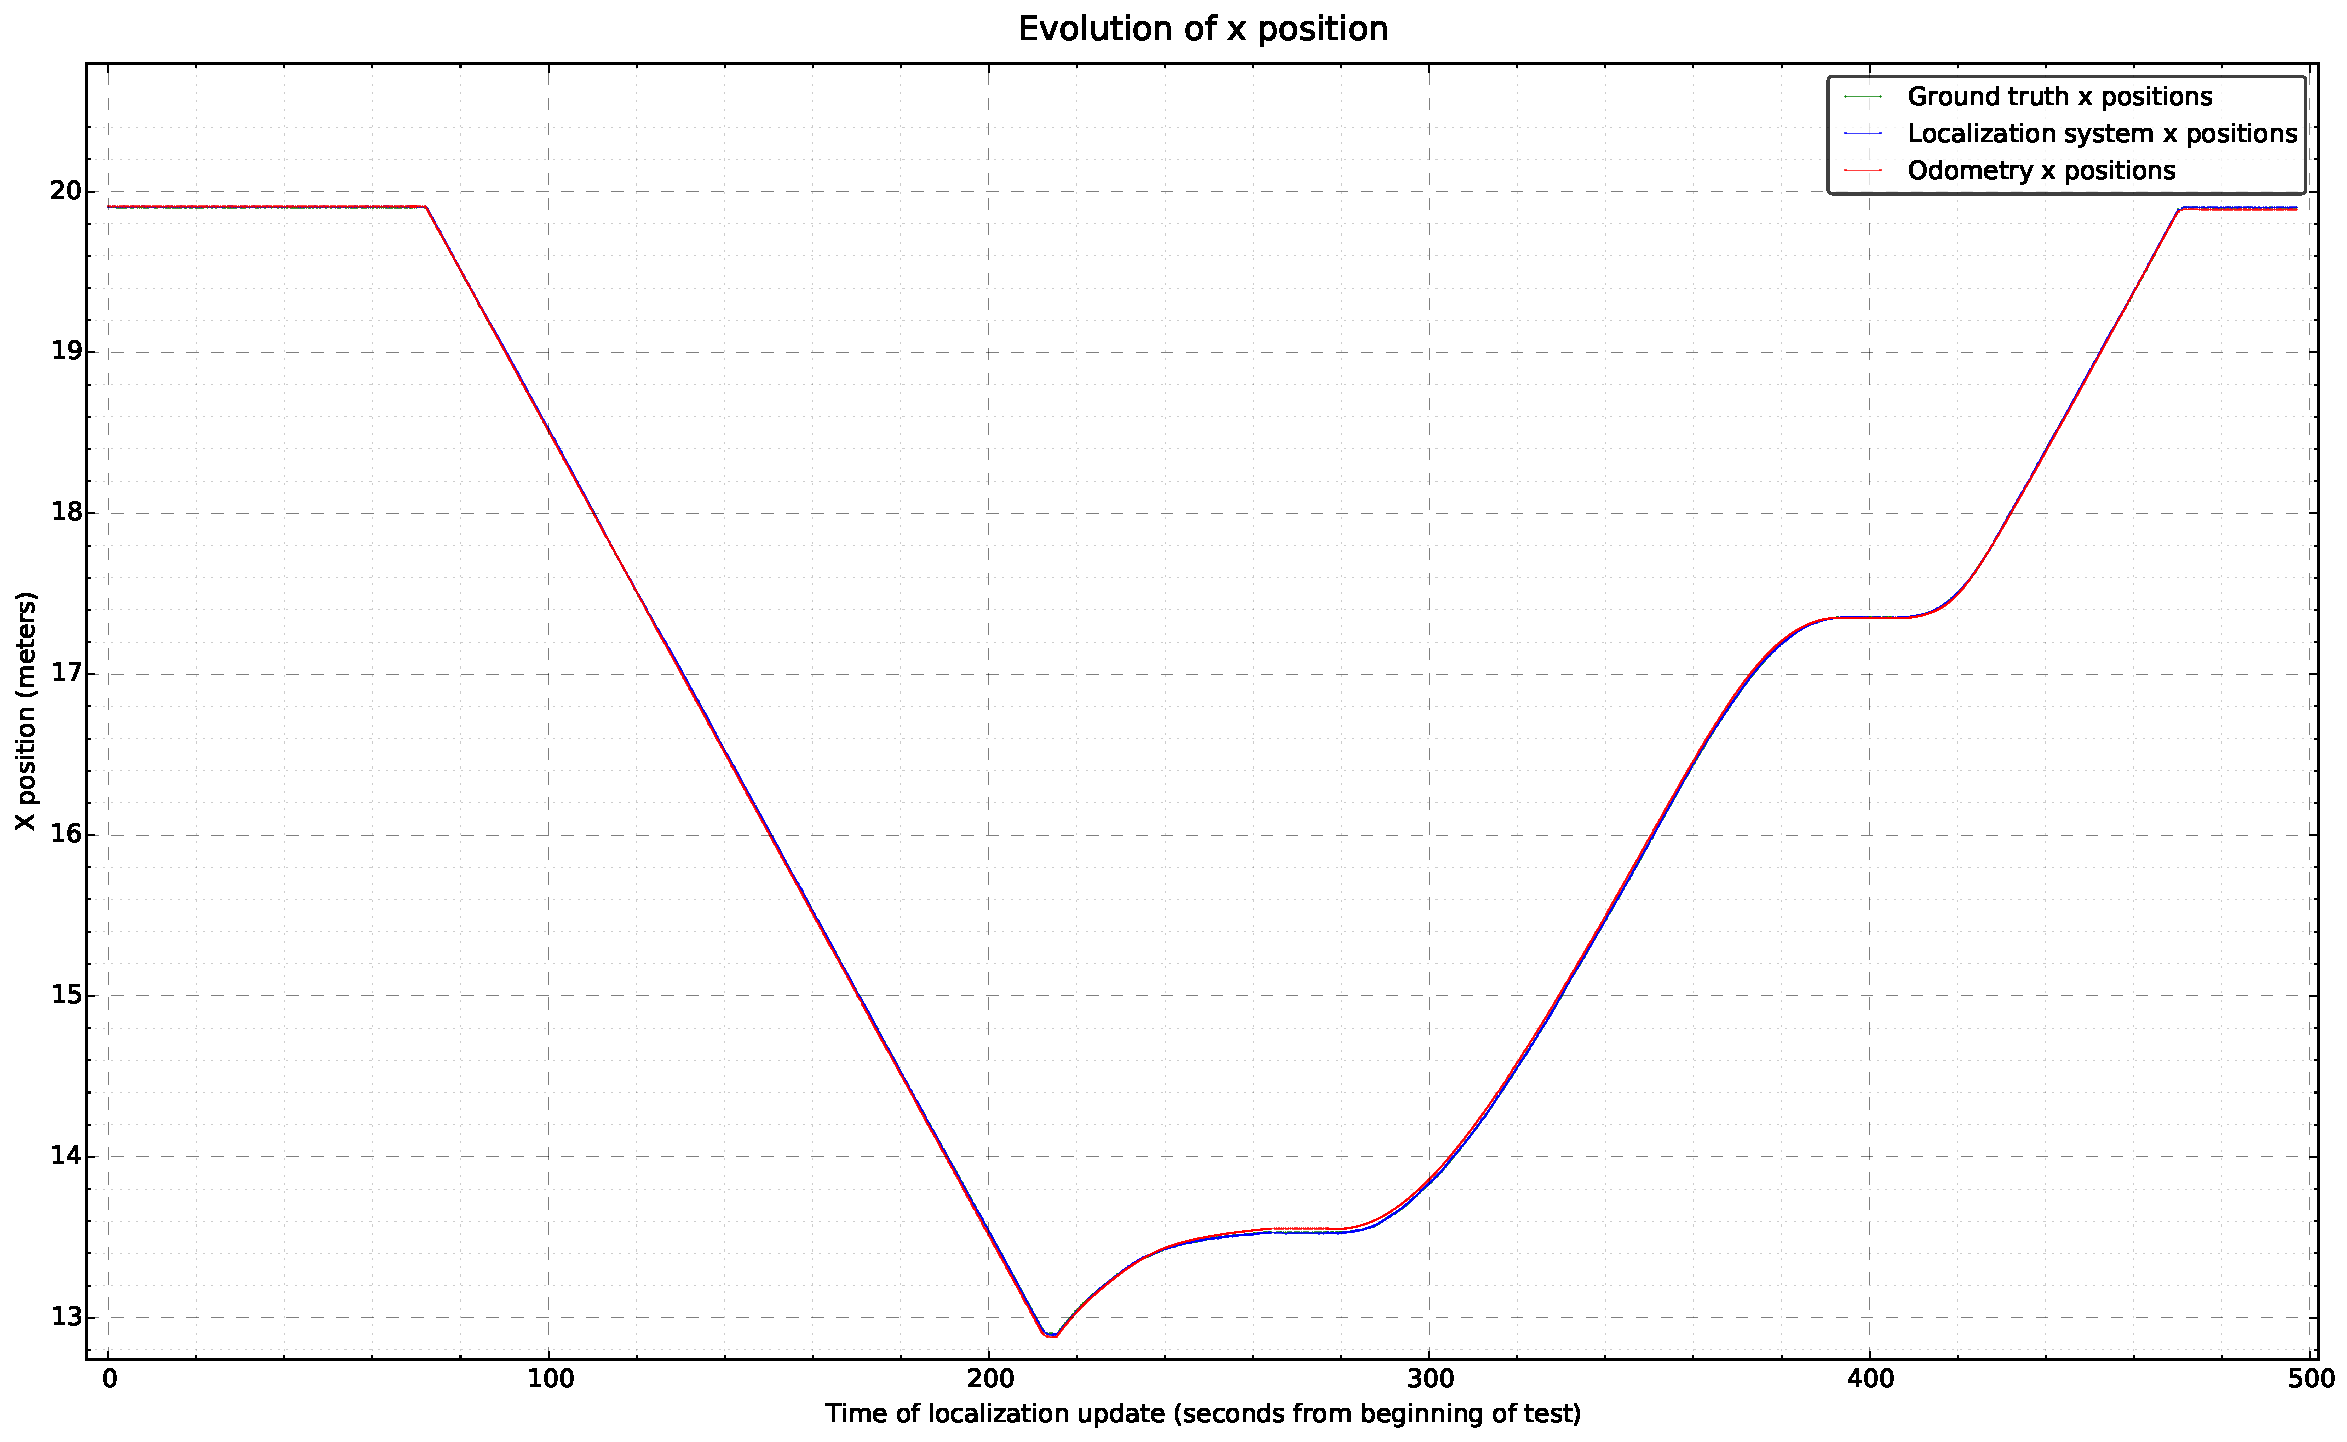
\includegraphics[width=0.69\textwidth]{appendices/tests-6dof/kinect/\currfilebase/graphs/robot-movement-path-position-evolution-x}
	\caption{Evolution of x position over time}
\end{figure}

\begin{figure}[H]
	\centering
	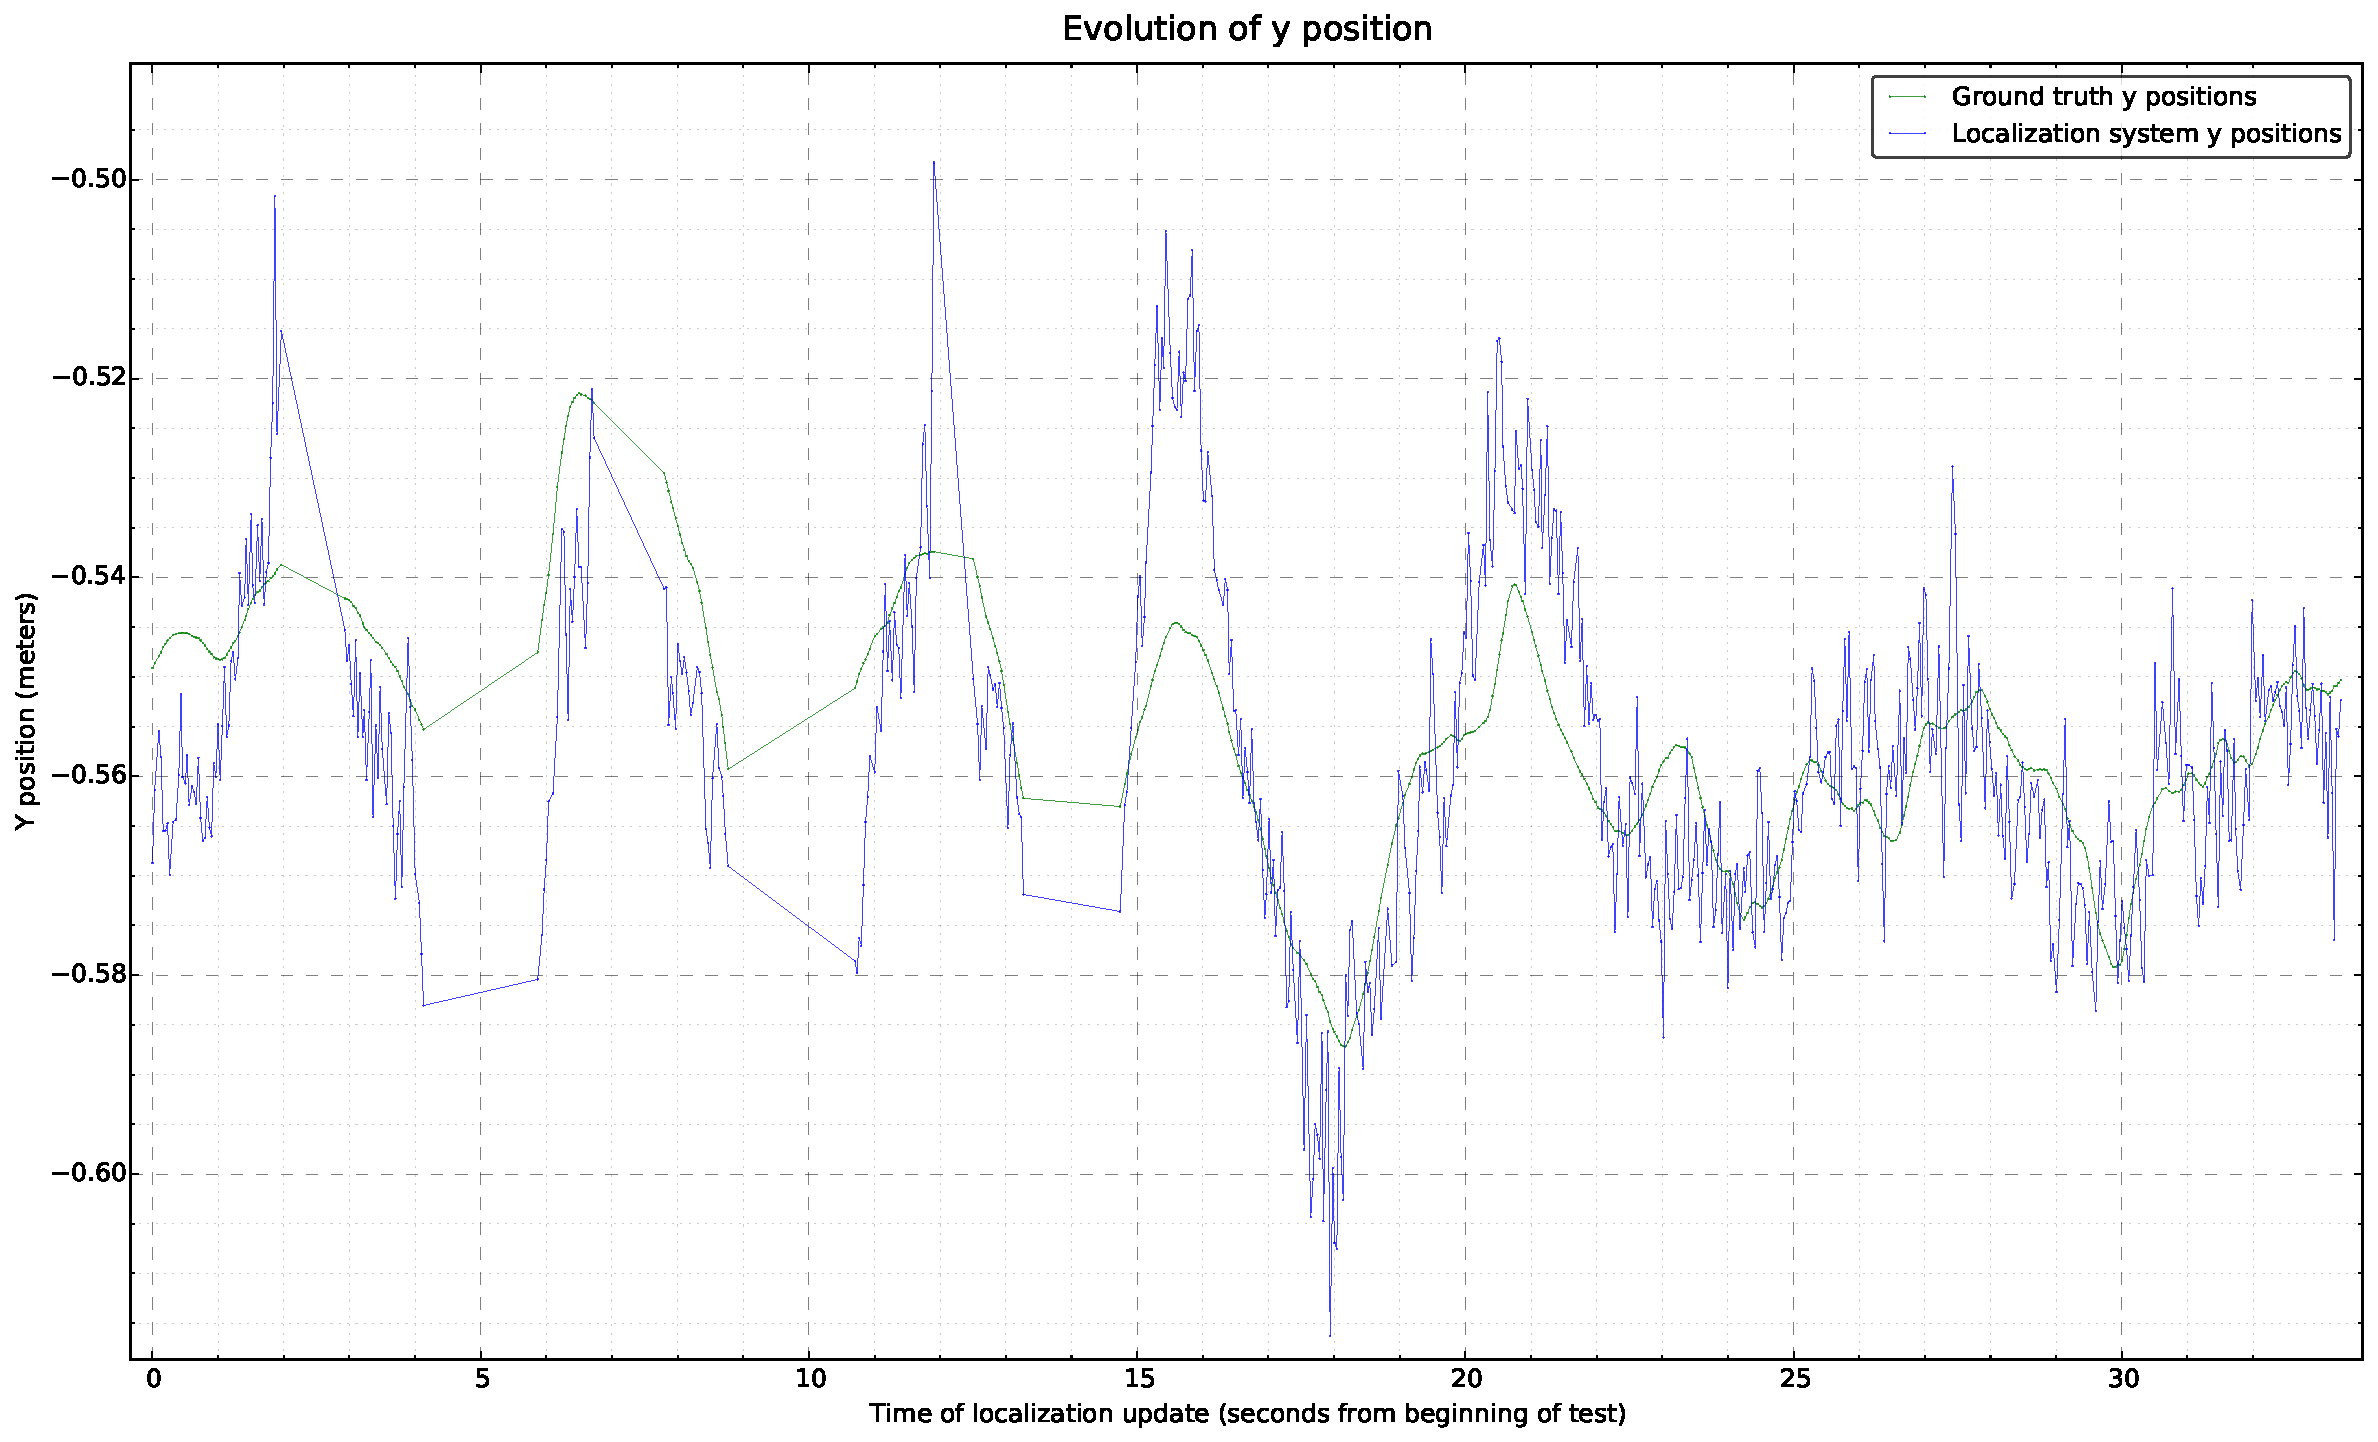
\includegraphics[width=0.69\textwidth]{appendices/tests-6dof/kinect/\currfilebase/graphs/robot-movement-path-position-evolution-y}
	\caption{Evolution of y position over time}
\end{figure}

\begin{figure}[H]
	\centering
	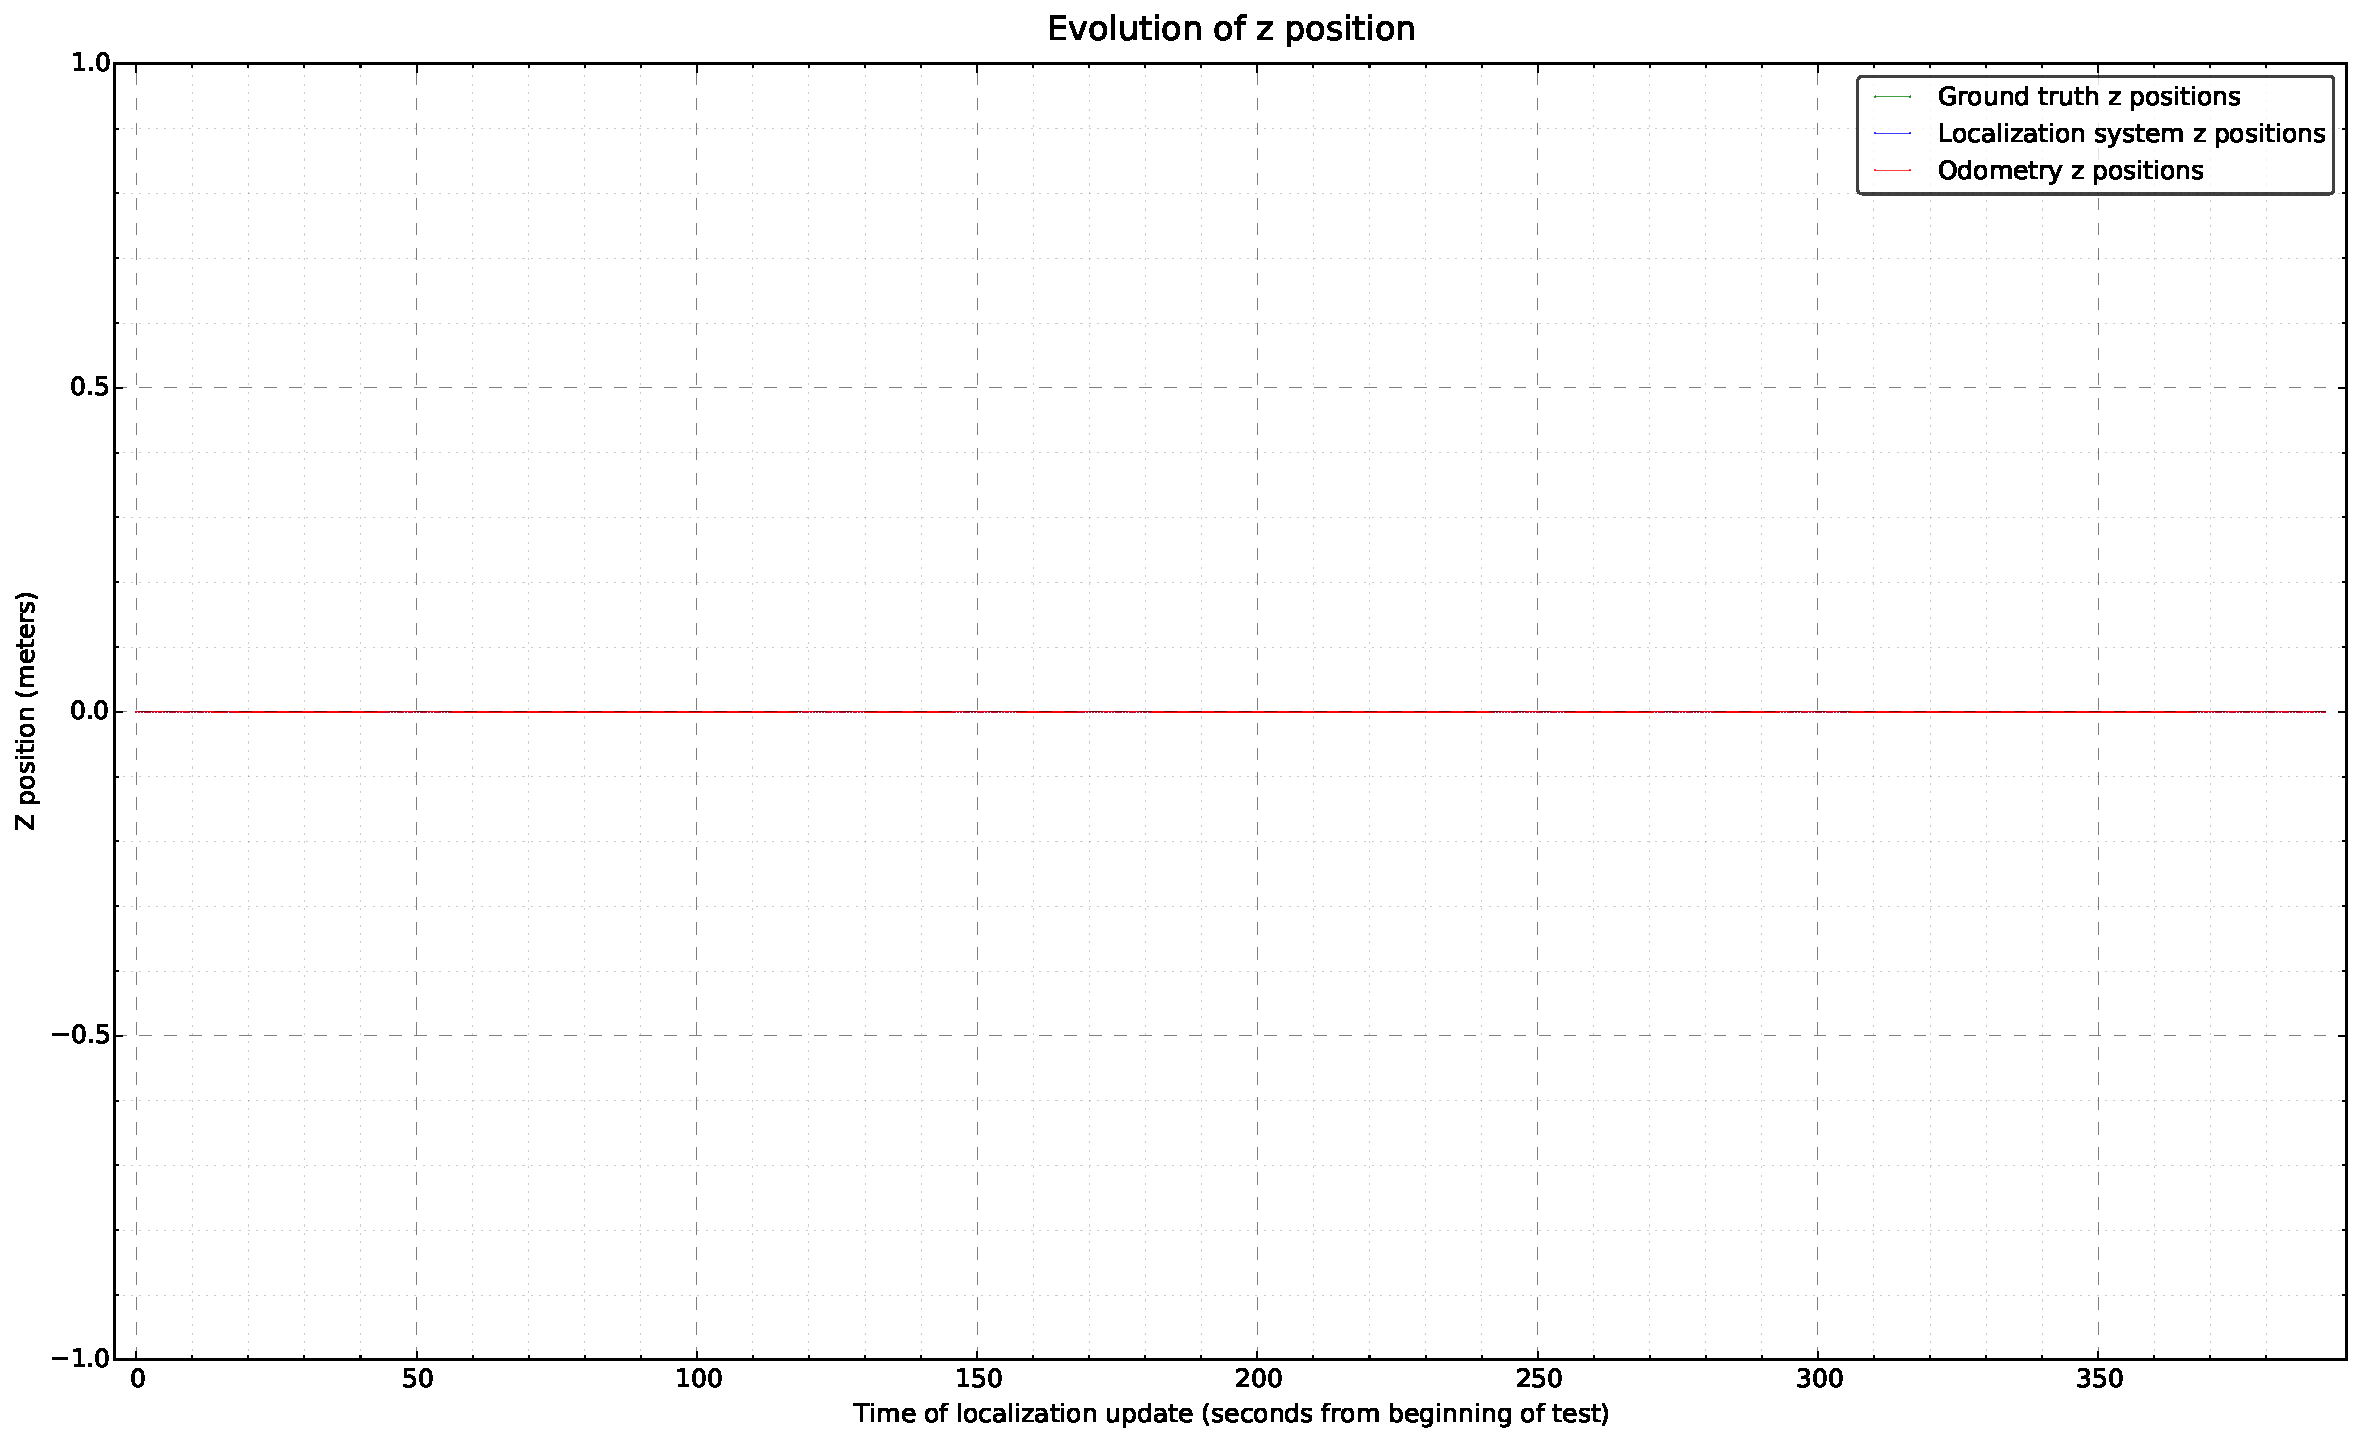
\includegraphics[width=0.69\textwidth]{appendices/tests-6dof/kinect/\currfilebase/graphs/robot-movement-path-position-evolution-z}
	\caption{Evolution of z position over time}
\end{figure}


%Distance derivatives
\begin{figure}[H]
	\centering
	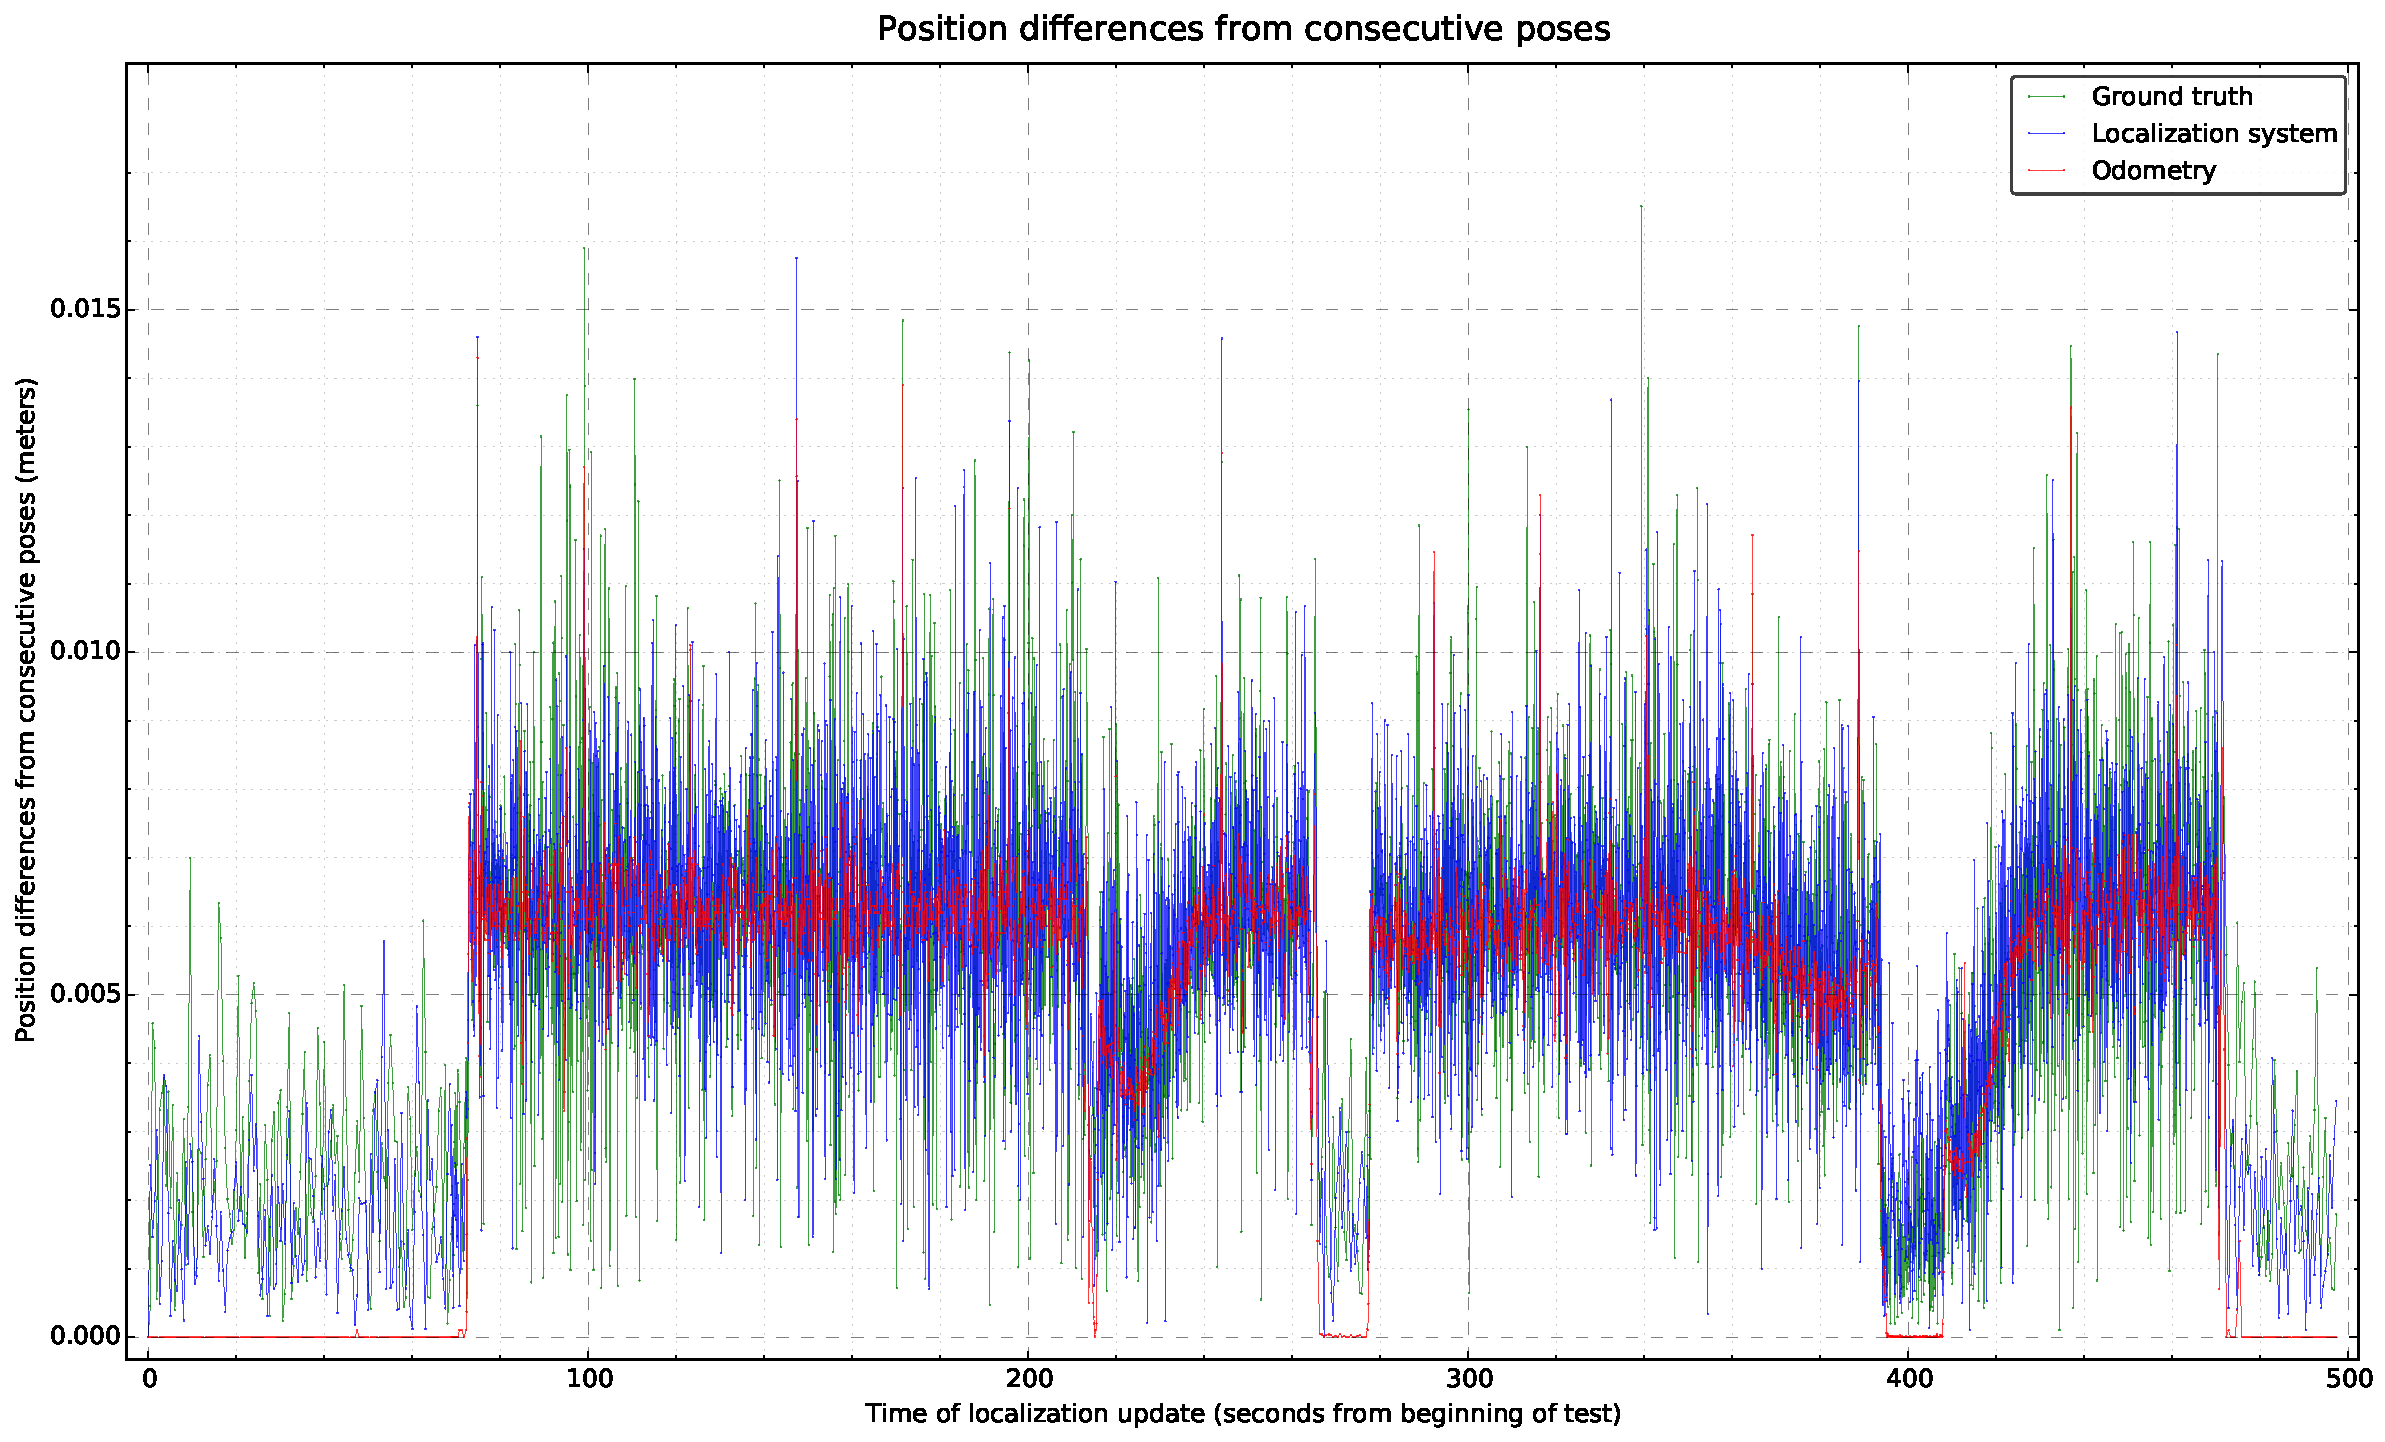
\includegraphics[width=0.69\textwidth]{appendices/tests-6dof/kinect/\currfilebase/graphs/robot-movement-path-position-differences}
	\caption{Distance traveled between consecutive pose estimations}
\end{figure}

\begin{figure}[H]
	\centering
	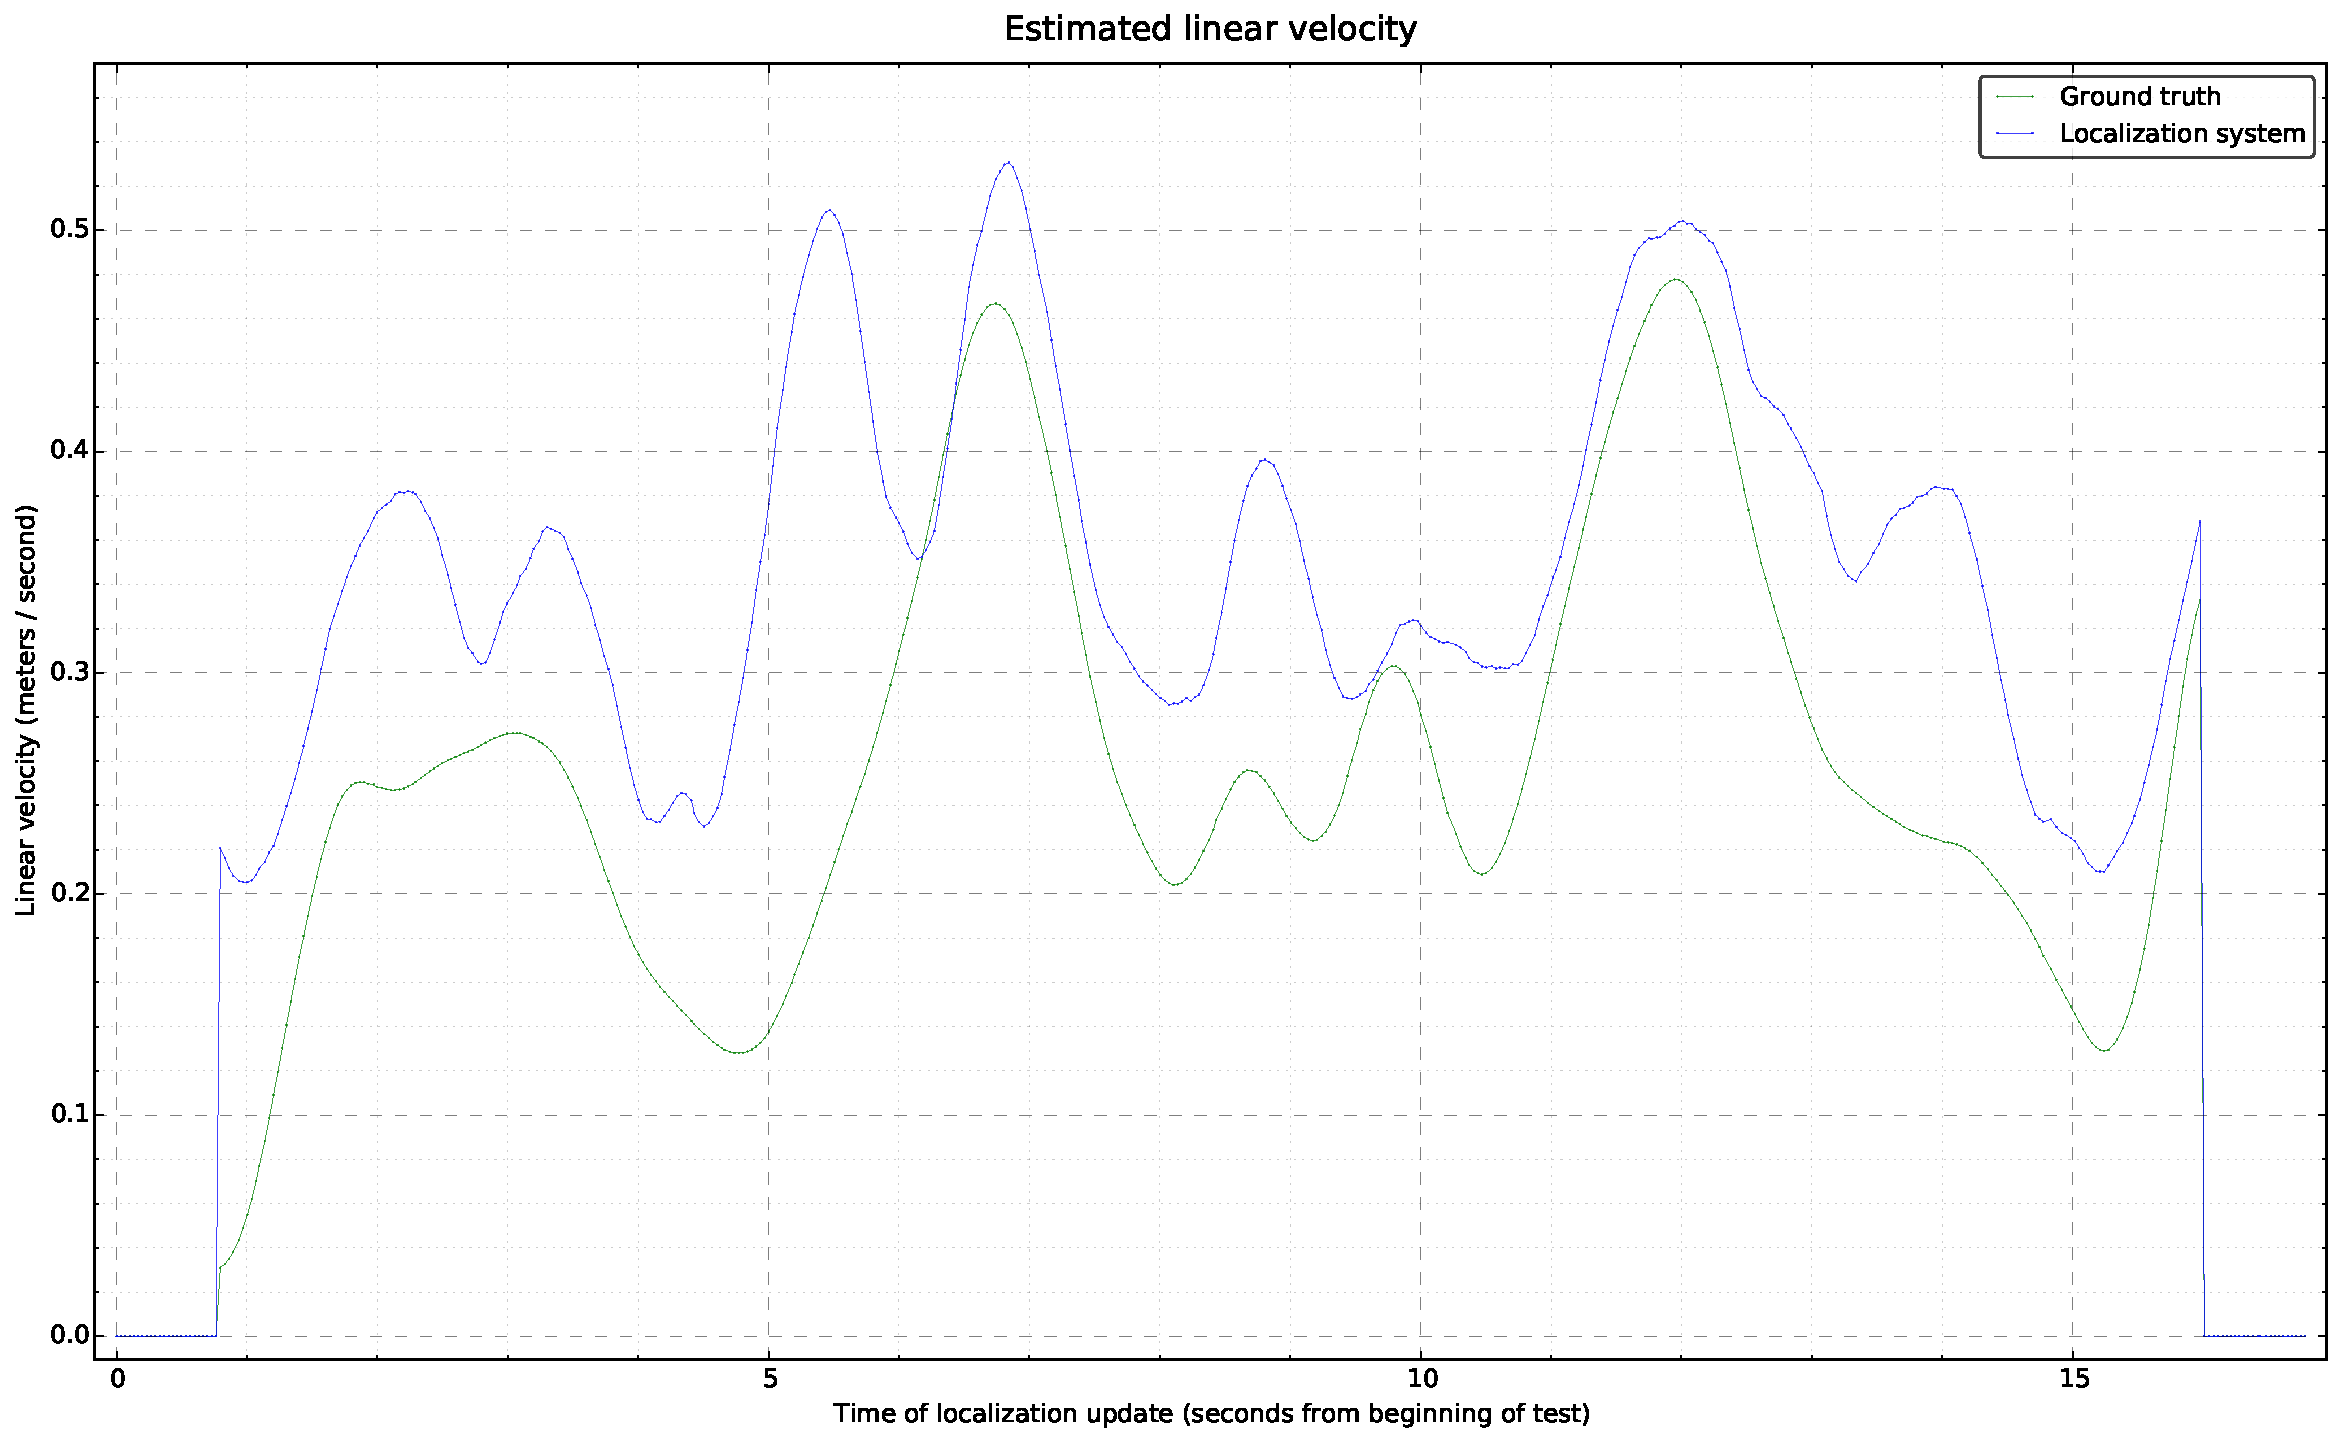
\includegraphics[width=0.69\textwidth]{appendices/tests-6dof/kinect/\currfilebase/graphs/robot-movement-path-linear-velocity}
	\caption{Estimated linear velocity}
\end{figure}

\begin{figure}[H]
	\centering
	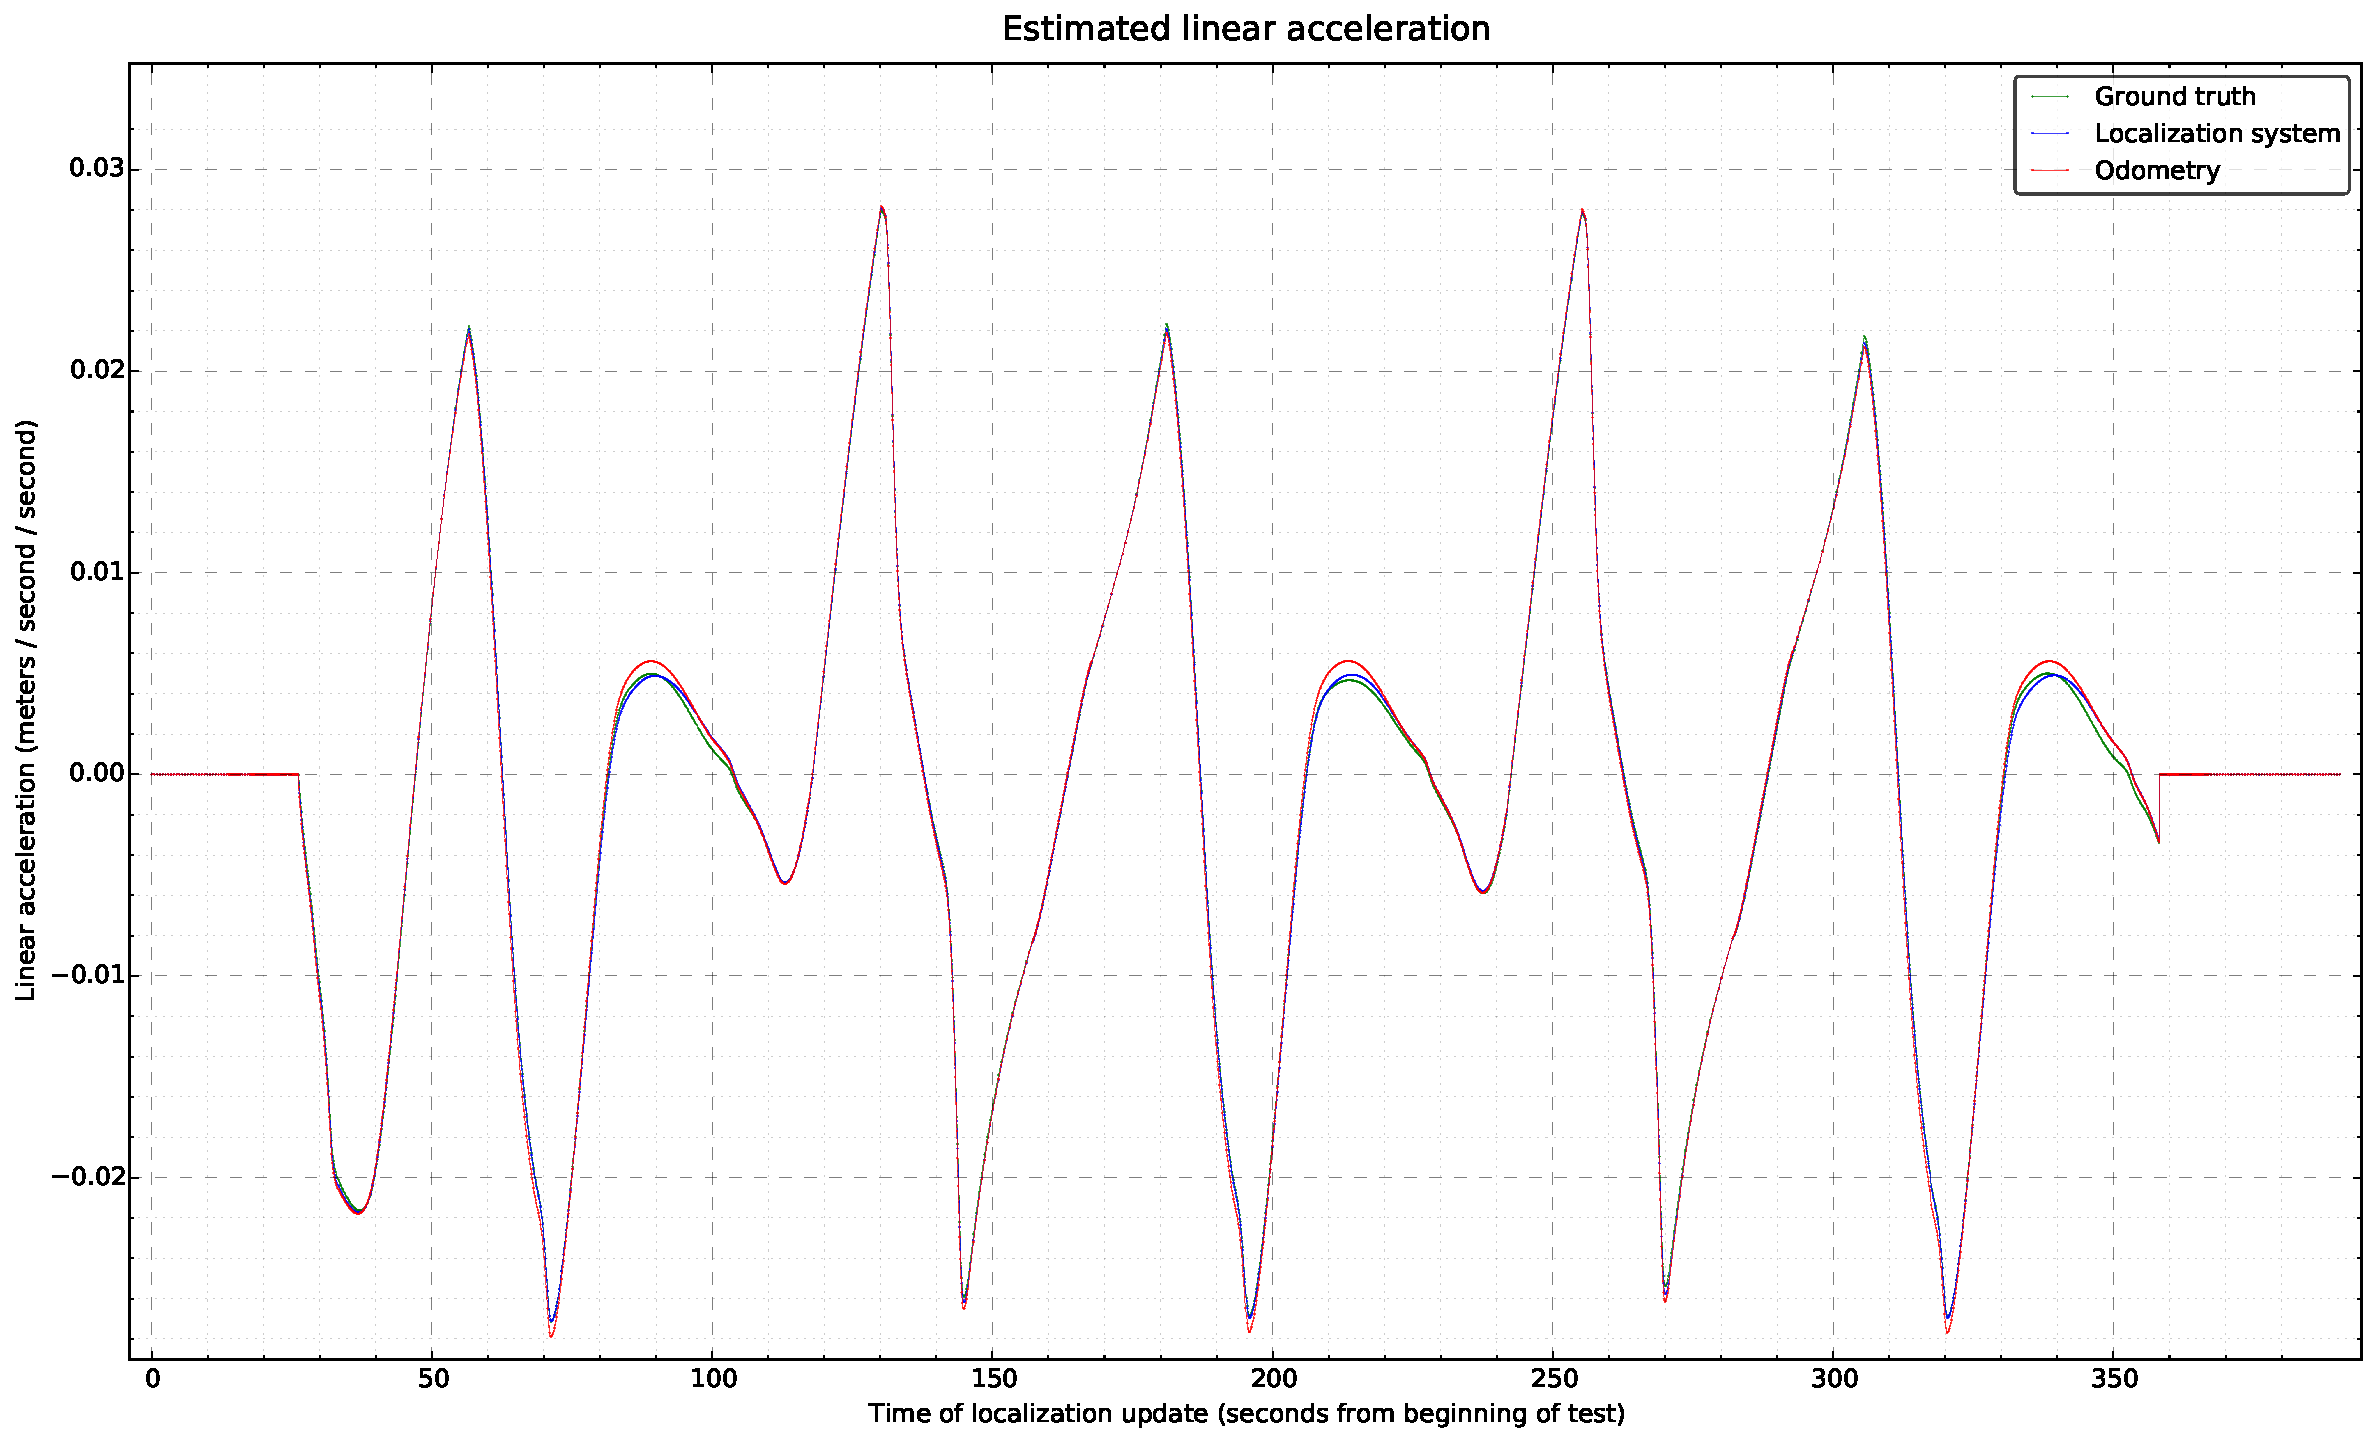
\includegraphics[width=0.69\textwidth]{appendices/tests-6dof/kinect/\currfilebase/graphs/robot-movement-path-linear-acceleration}
	\caption{Estimated linear acceleration}
\end{figure}


%Angular derivatives
\begin{figure}[H]
	\centering
	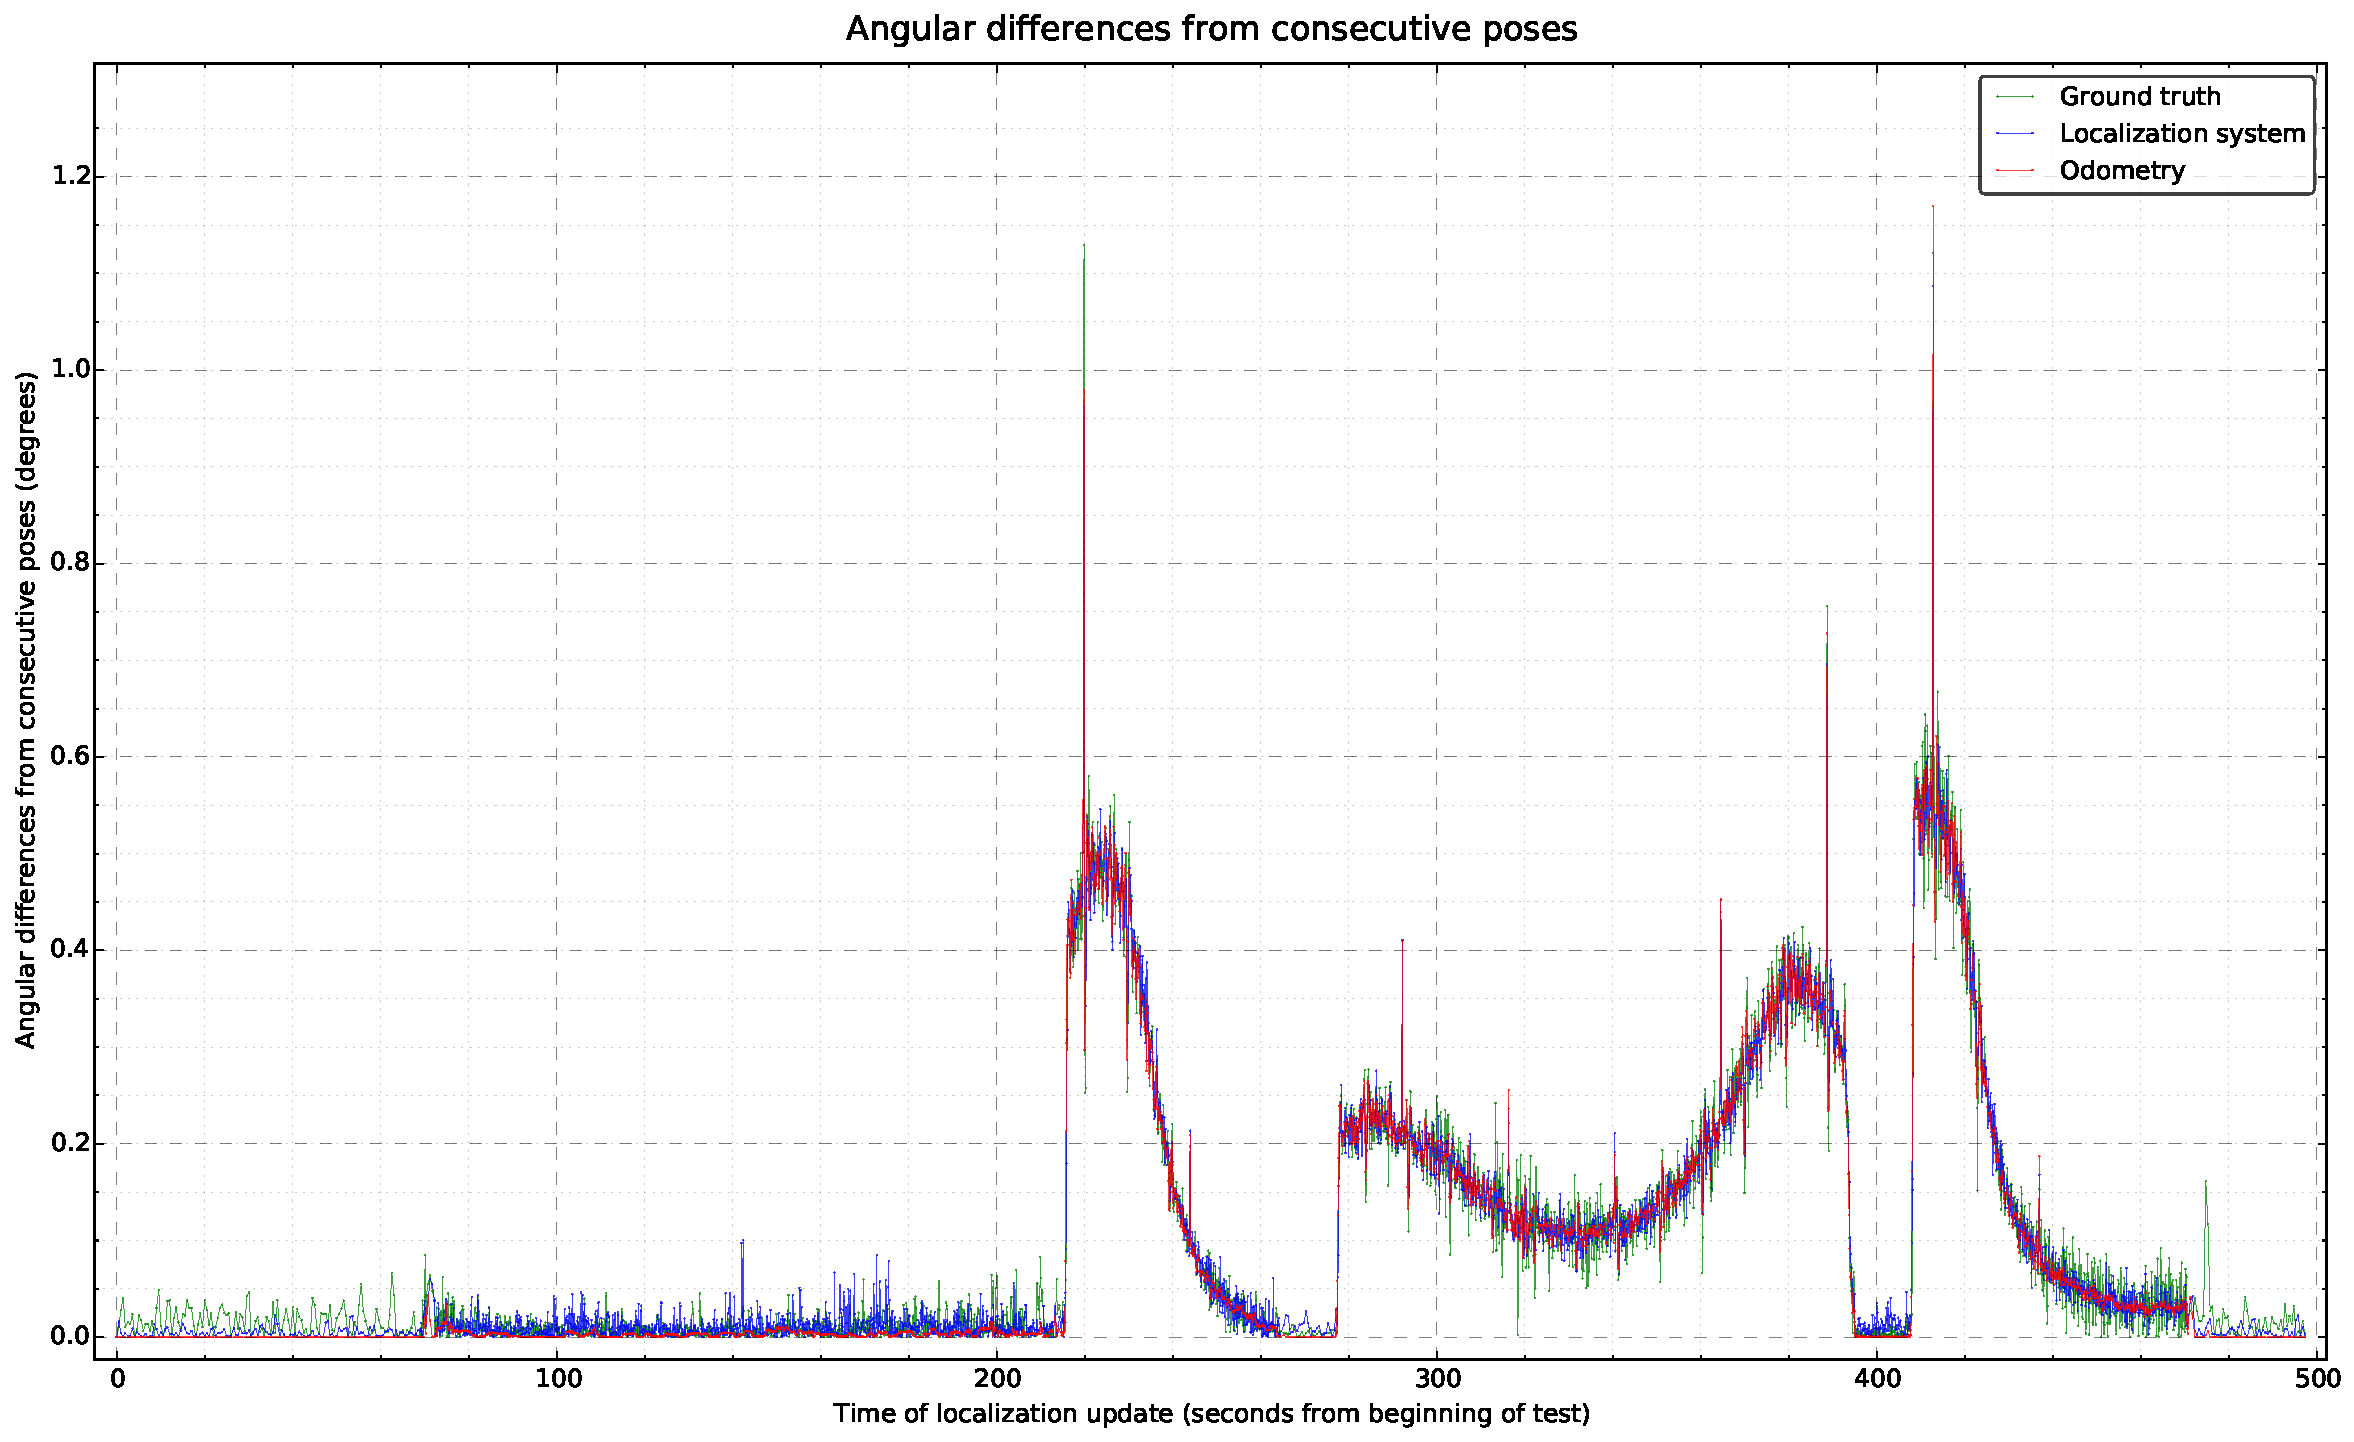
\includegraphics[width=0.69\textwidth]{appendices/tests-6dof/kinect/\currfilebase/graphs/robot-movement-path-angular-differences}
	\caption{Angular differences between consecutive pose estimations}
\end{figure}

\begin{figure}[H]
	\centering
	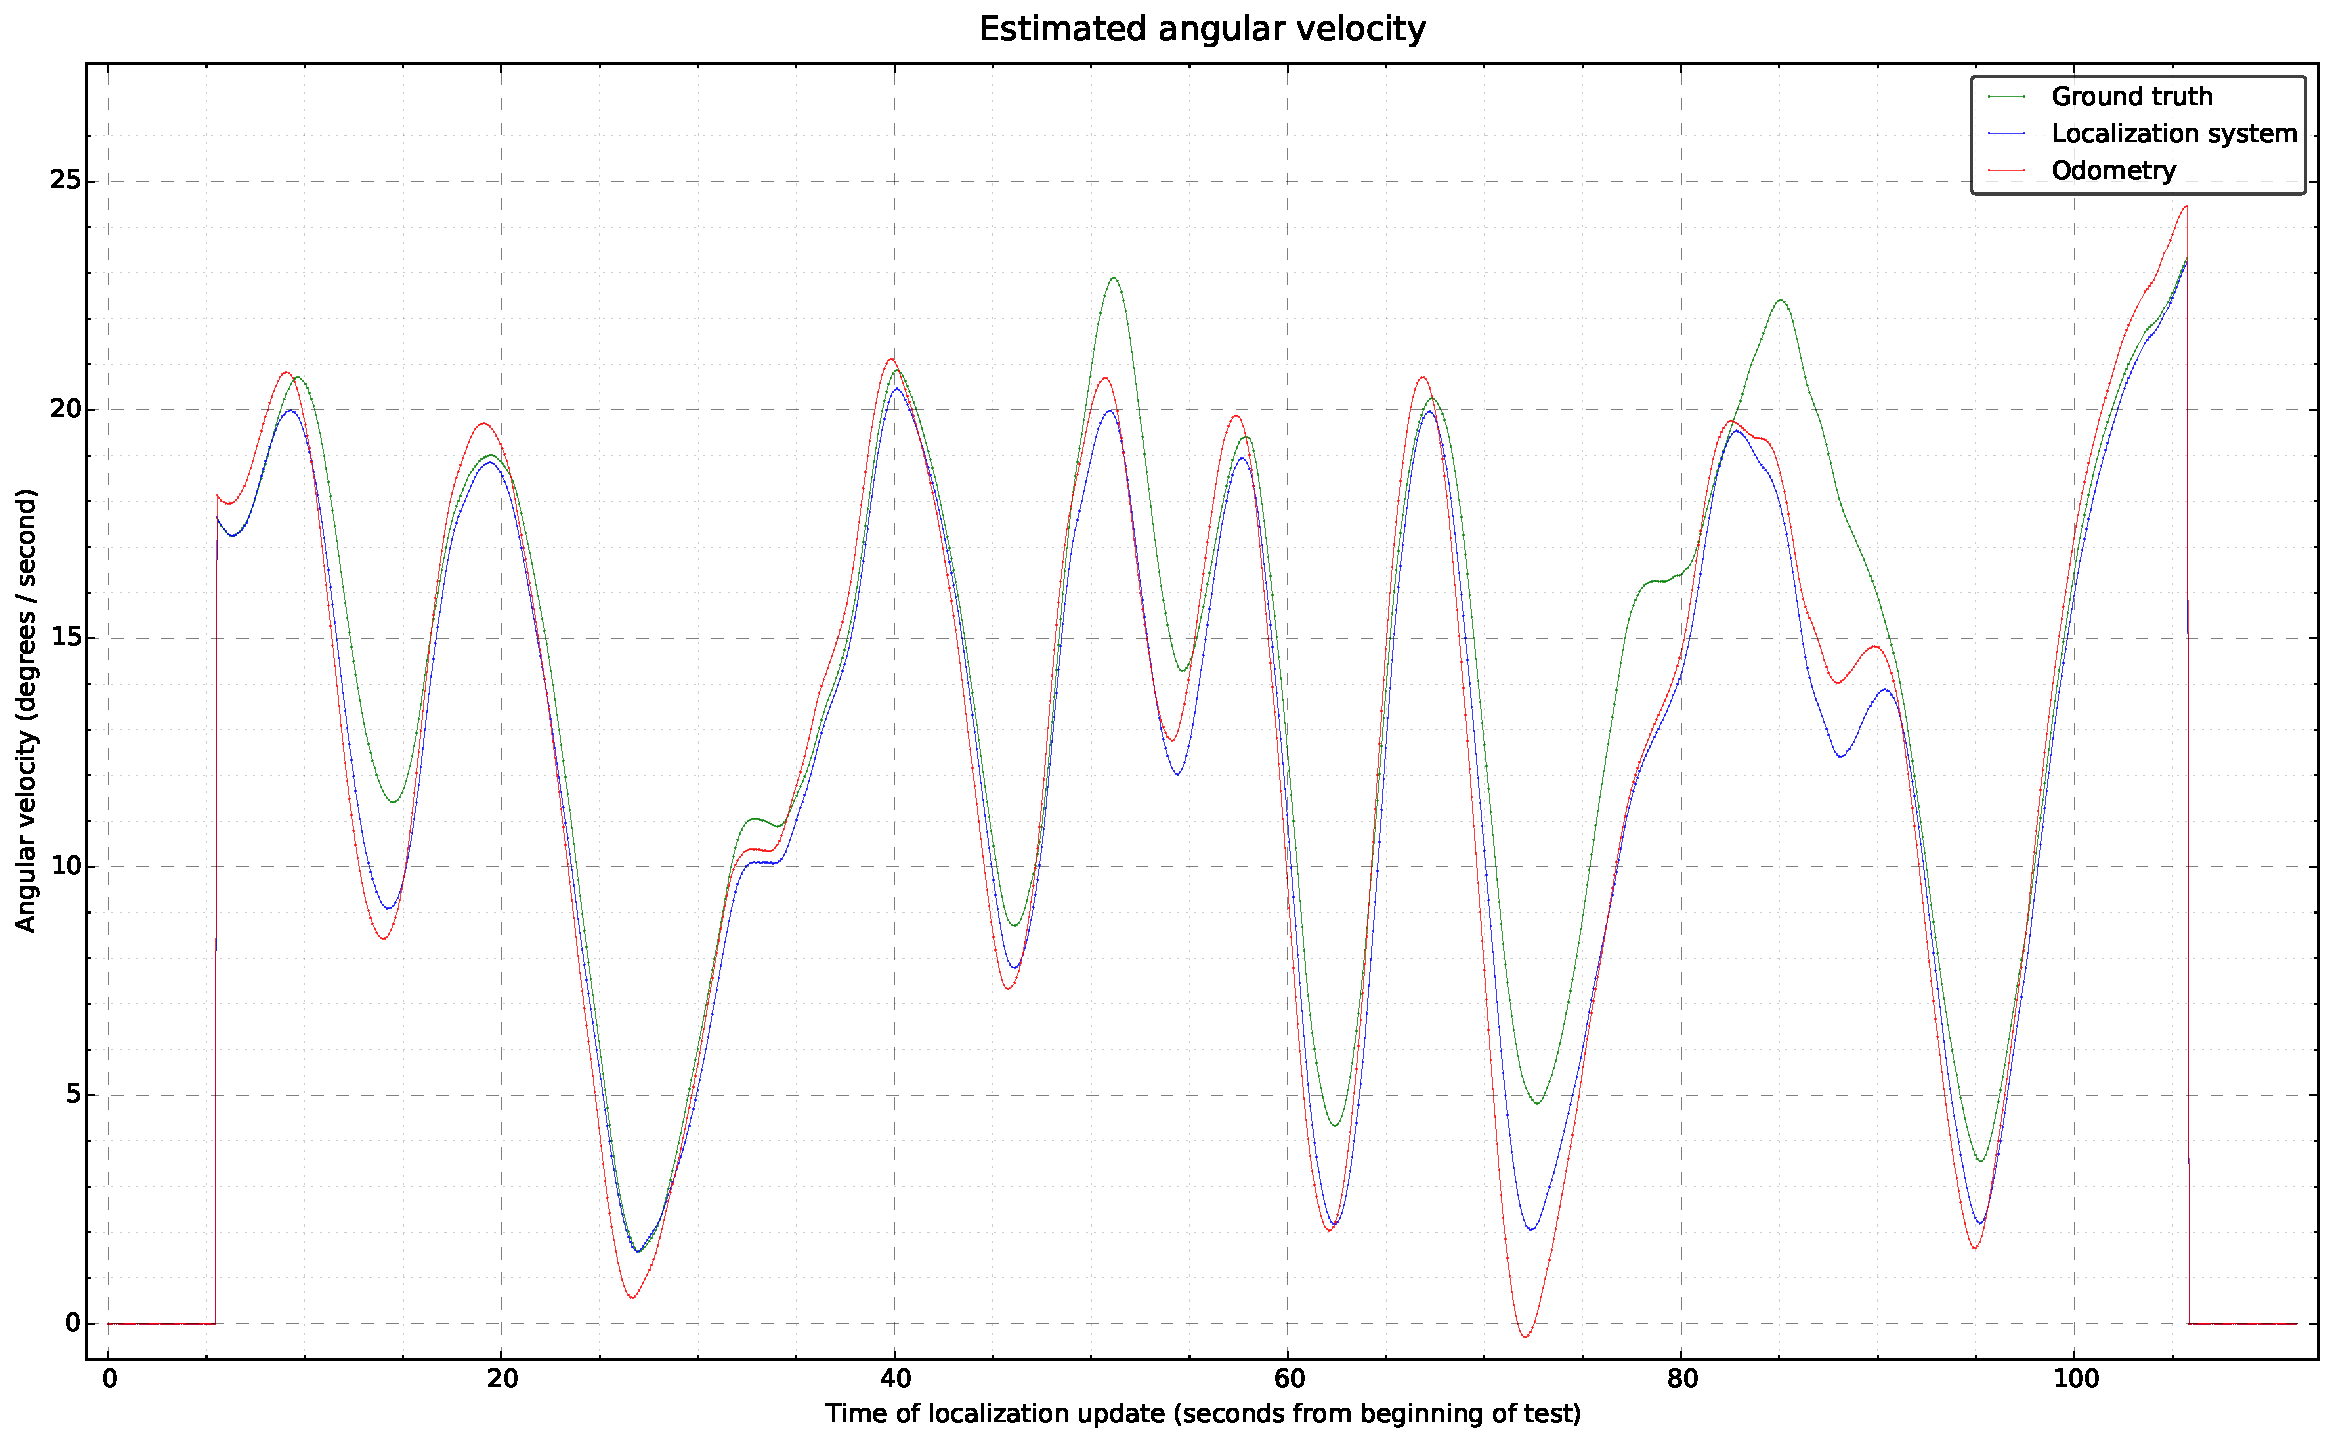
\includegraphics[width=0.69\textwidth]{appendices/tests-6dof/kinect/\currfilebase/graphs/robot-movement-path-angular-velocity}
	\caption{Estimated angular velocity}
\end{figure}

\begin{figure}[H]
	\centering
	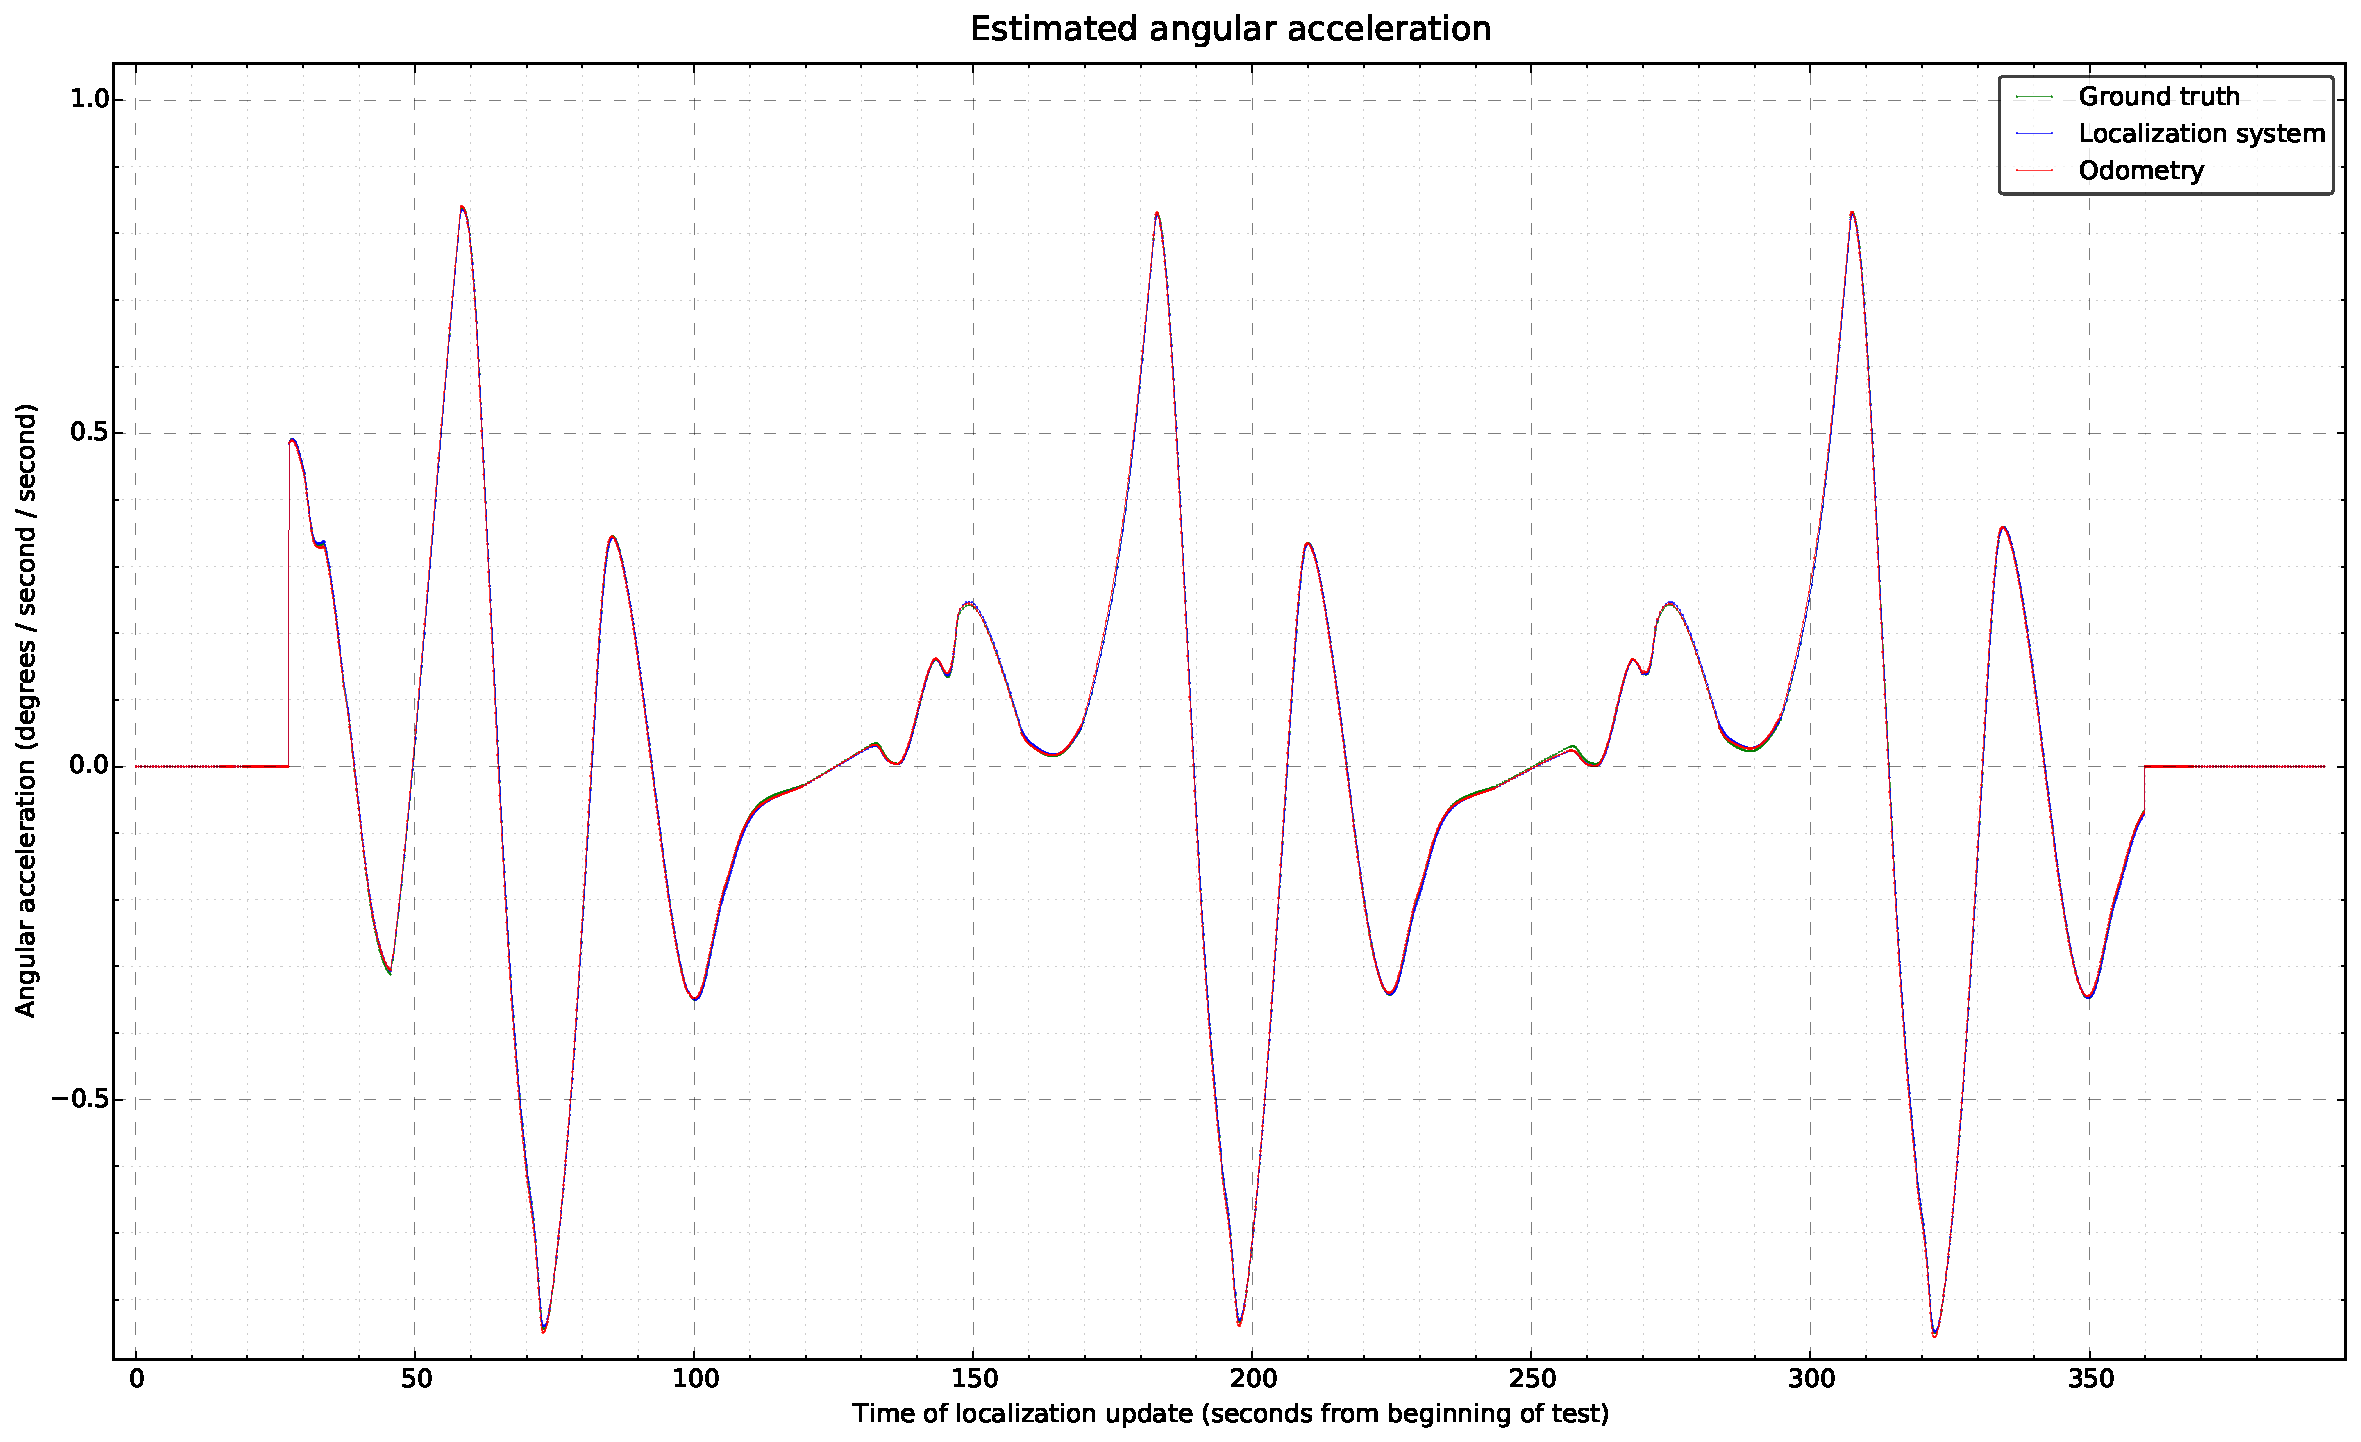
\includegraphics[width=0.69\textwidth]{appendices/tests-6dof/kinect/\currfilebase/graphs/robot-movement-path-angular-acceleration}
	\caption{Estimated angular acceleration}
\end{figure}


%Translation errors
\begin{figure}[H]
	\centering
	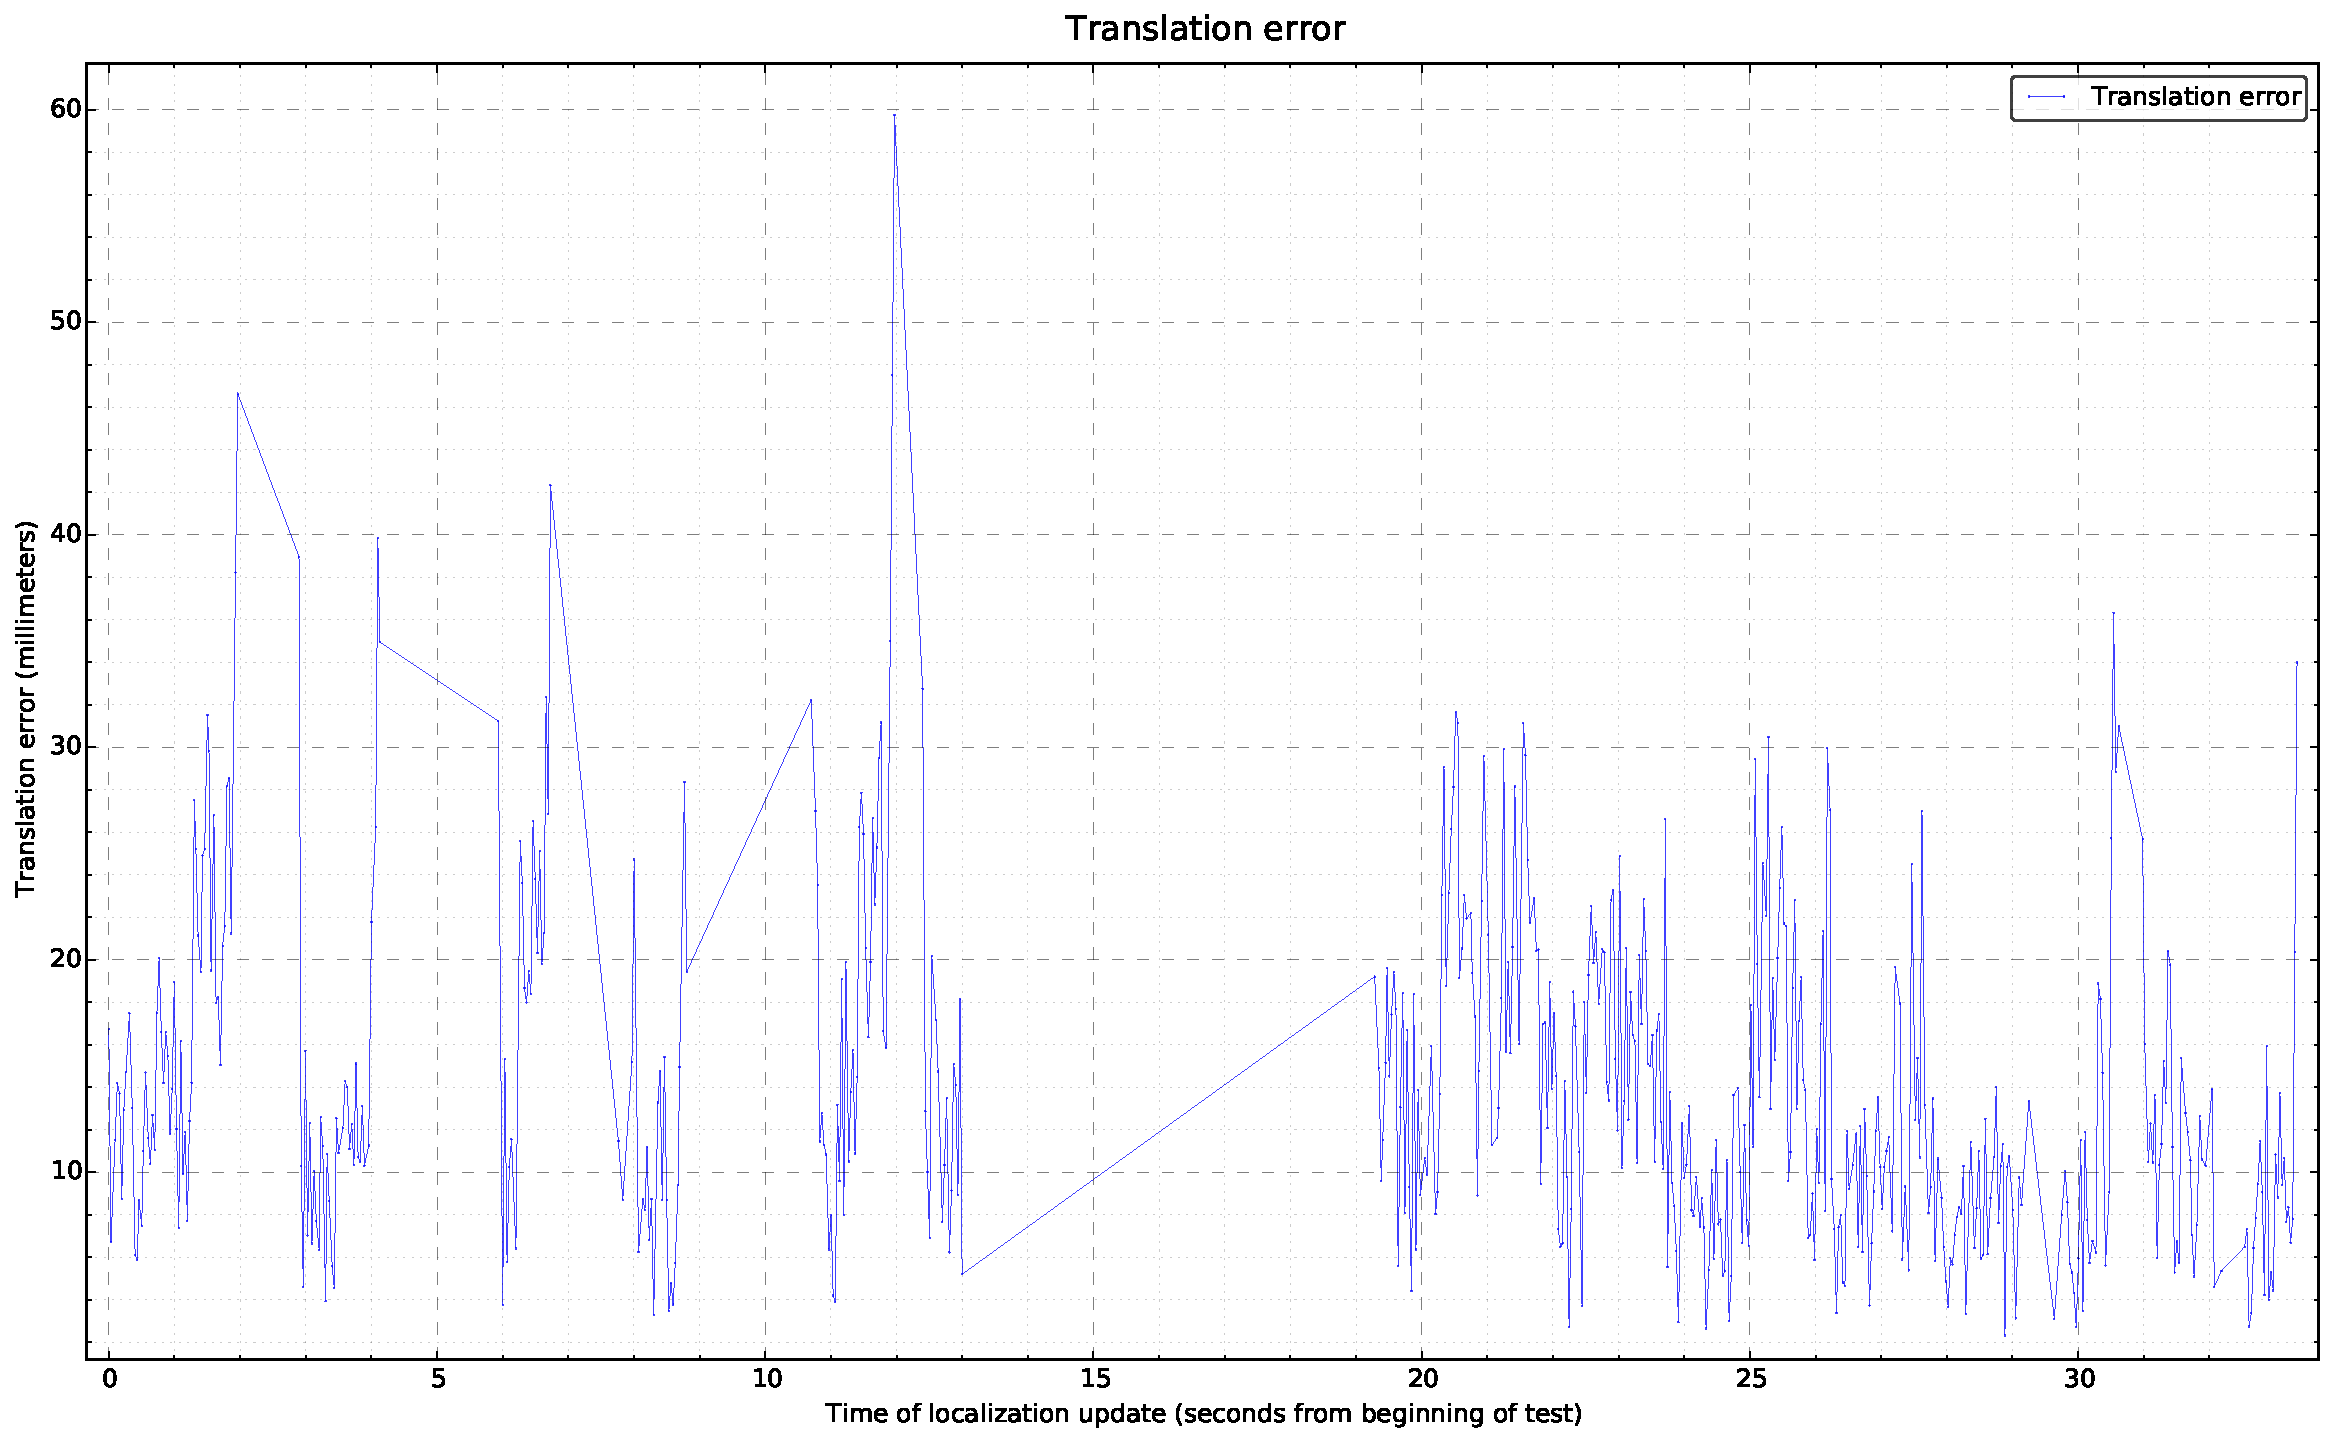
\includegraphics[width=0.69\textwidth]{appendices/tests-6dof/kinect/\currfilebase/graphs/translation-error-millimeters}
	\caption{Localization system translation errors}
\end{figure}


%Translation errors components
\begin{figure}[H]
	\centering
	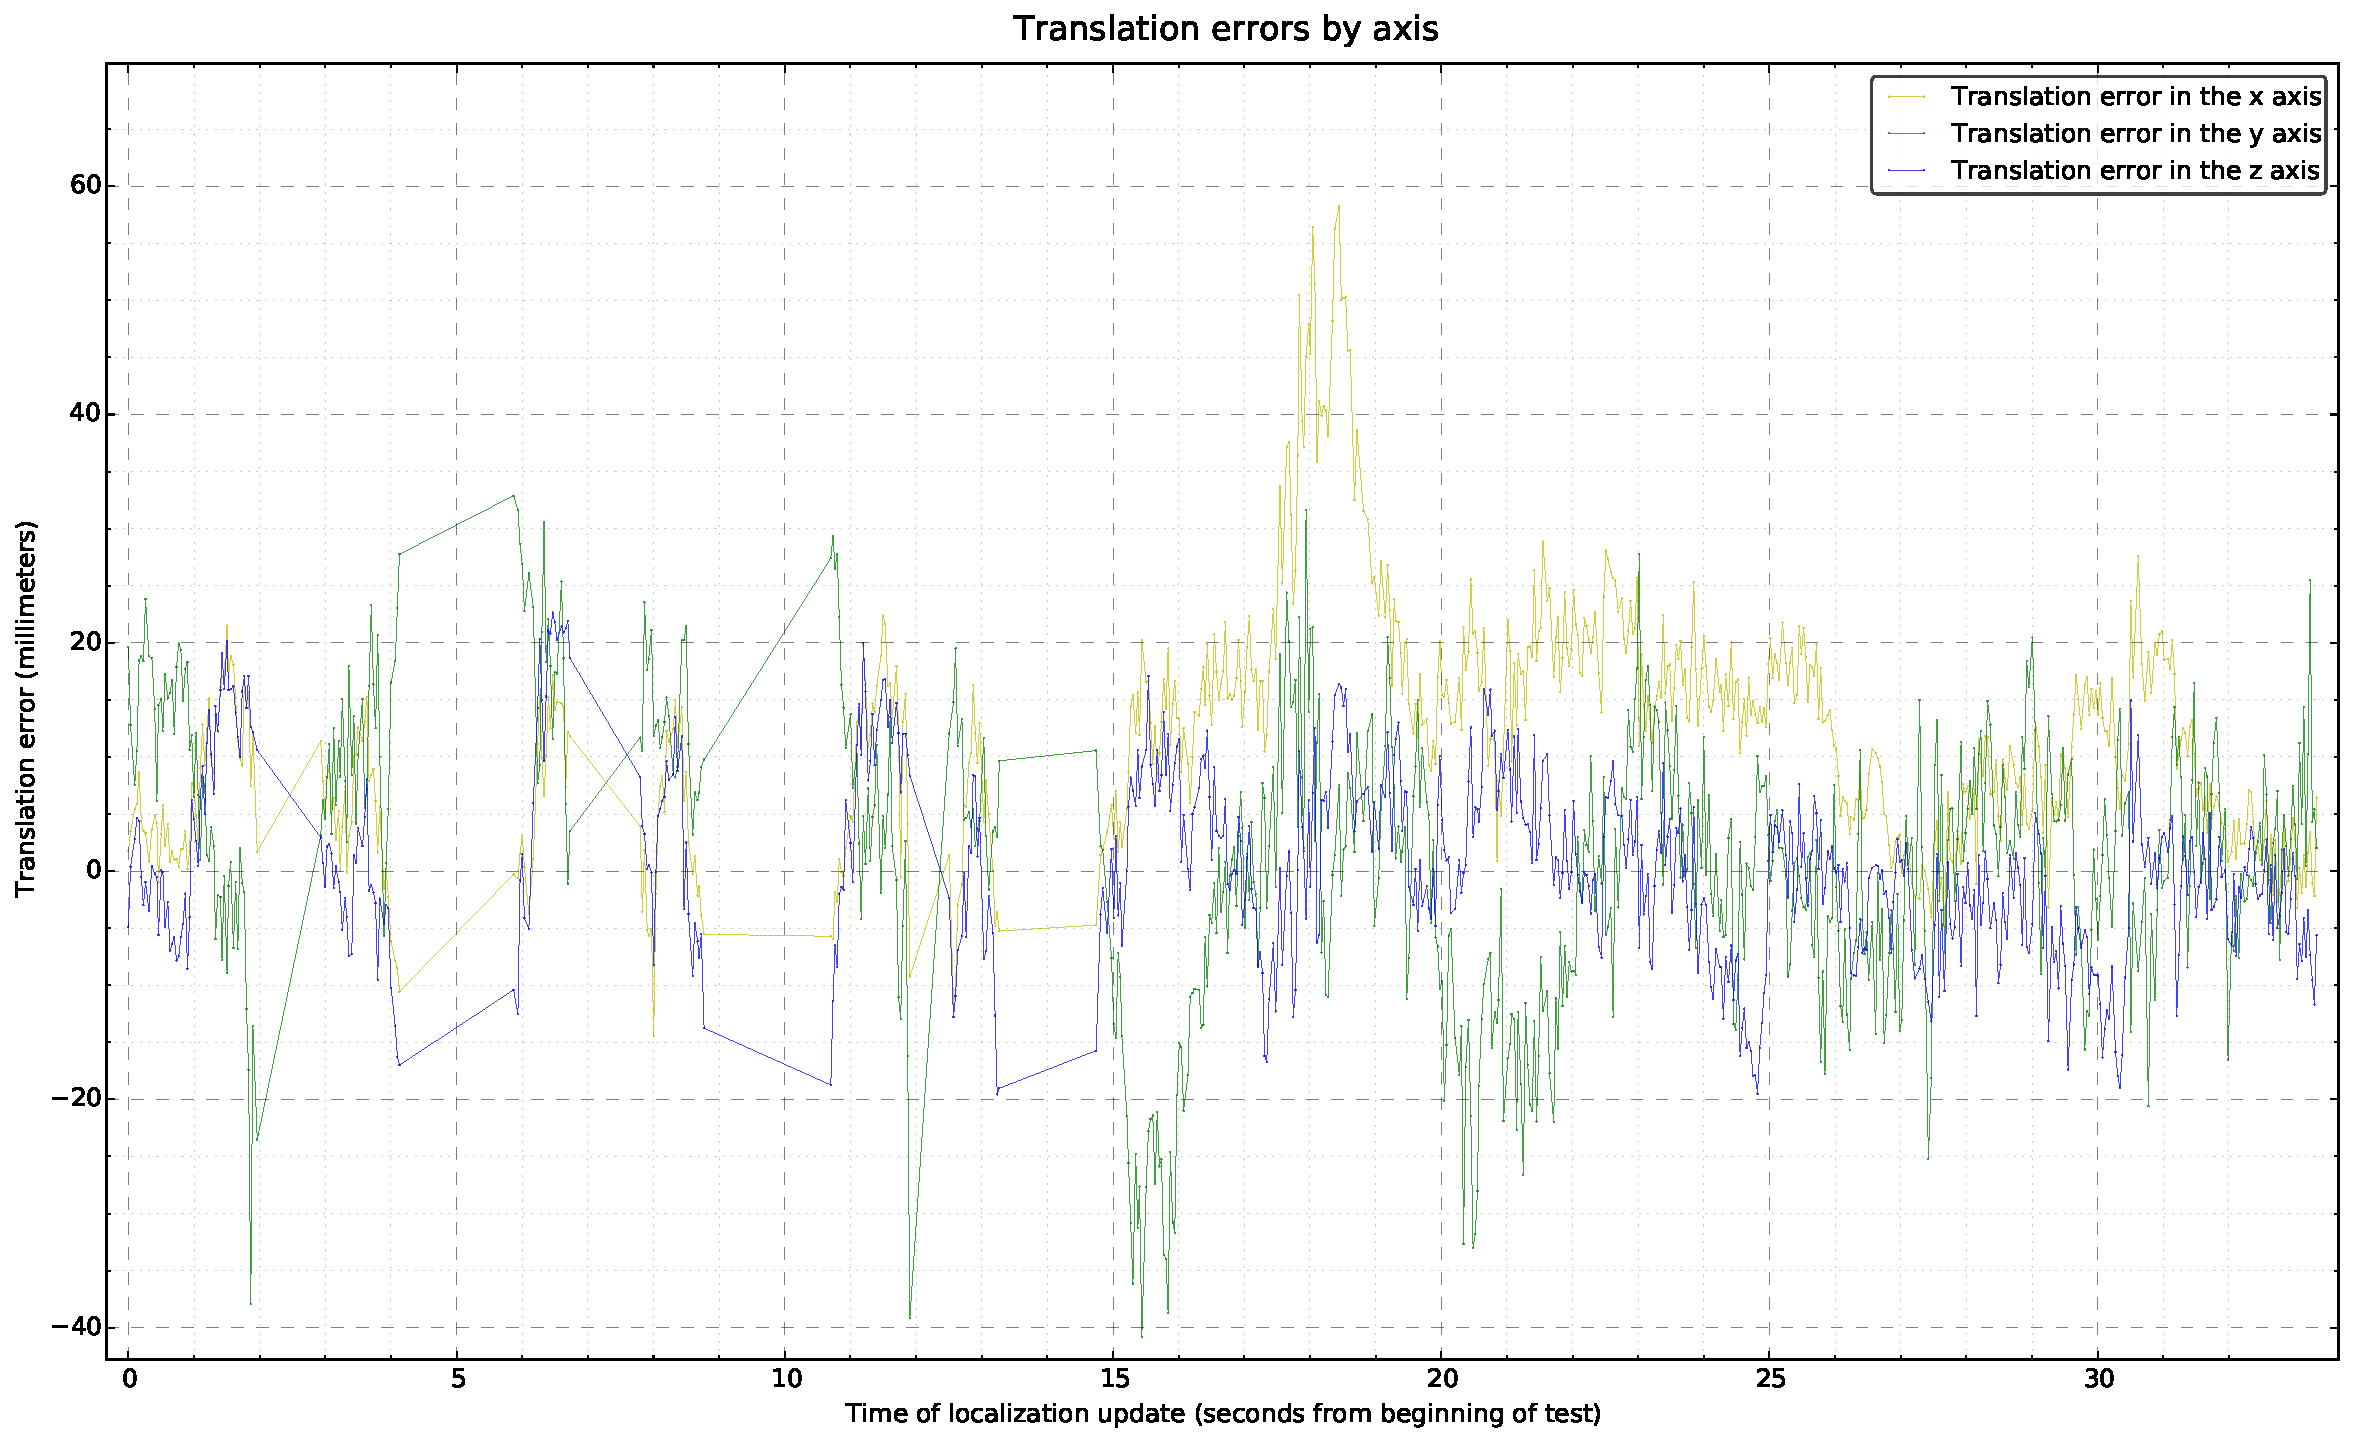
\includegraphics[width=0.69\textwidth]{appendices/tests-6dof/kinect/\currfilebase/graphs/translation-error-components-millimeters}
	\caption{Localization system translation errors components}
\end{figure}


%Translation errors distributions
\begin{figure}[H]
	\centering
	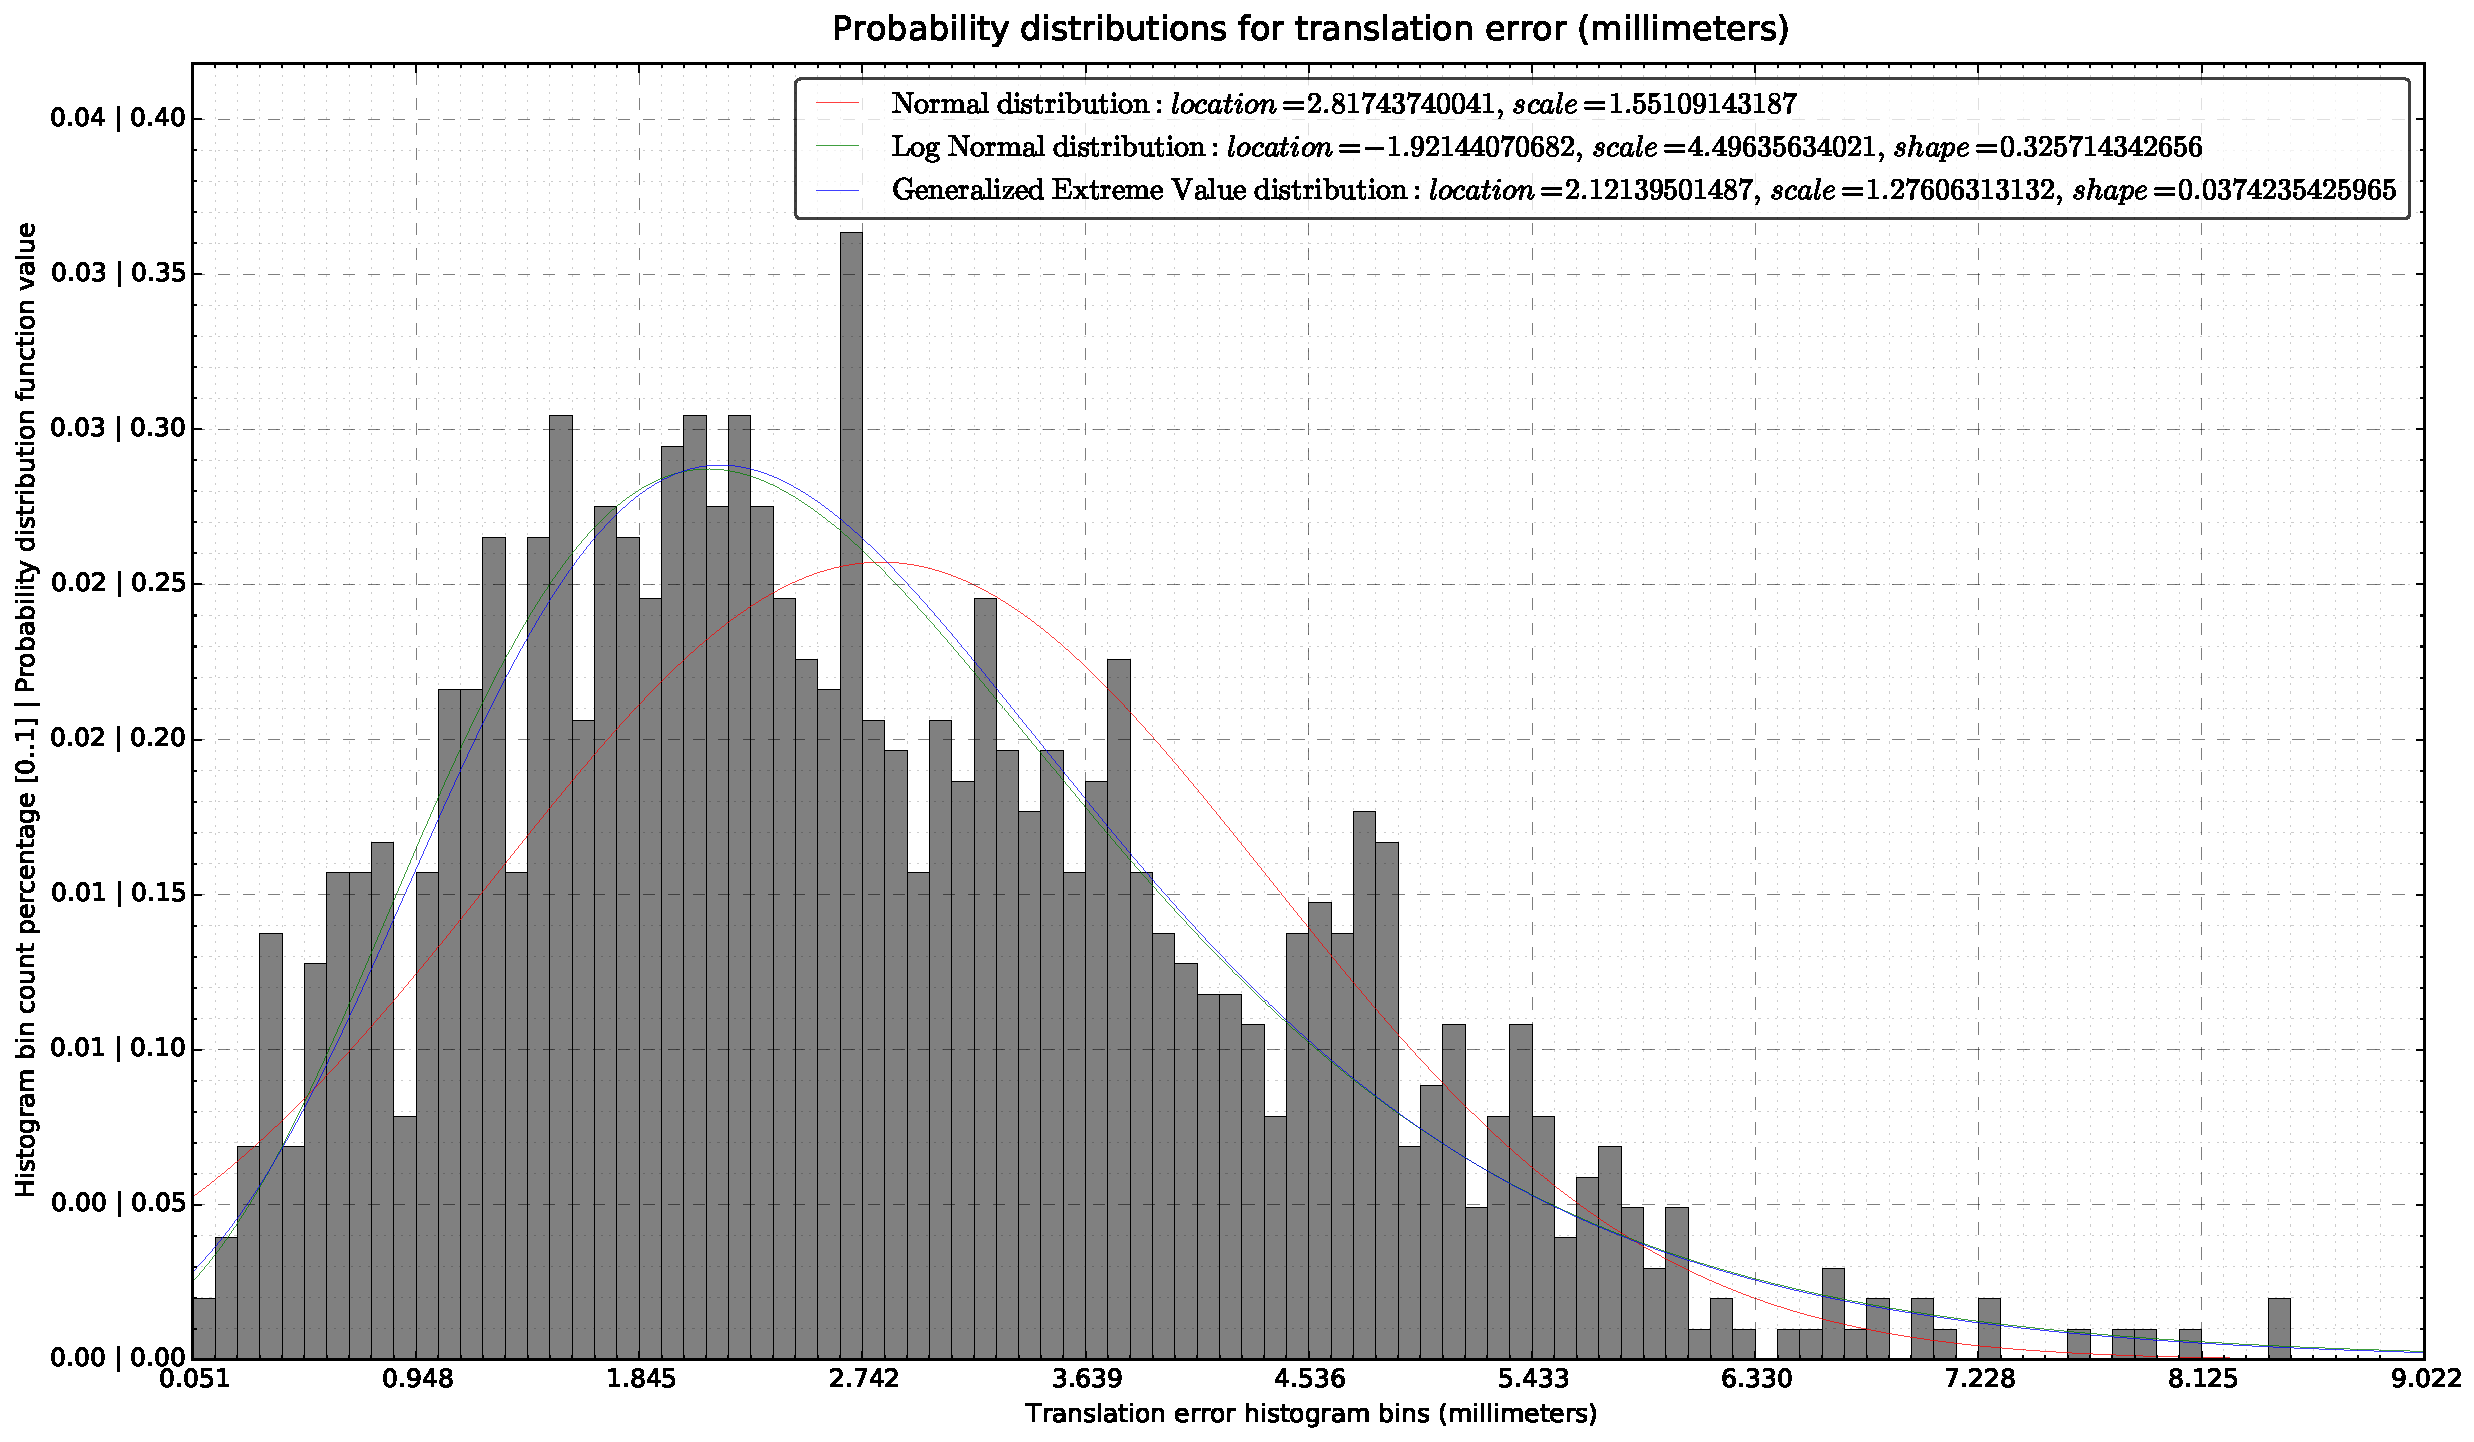
\includegraphics[width=0.73\textwidth]{appendices/tests-6dof/kinect/\currfilebase/graphs/translation-error-millimeters-distributions}
	\caption{Probability distributions for the localization system translation errors}
\end{figure}



%Angular errors axis
\begin{figure}[H]
	\centering
	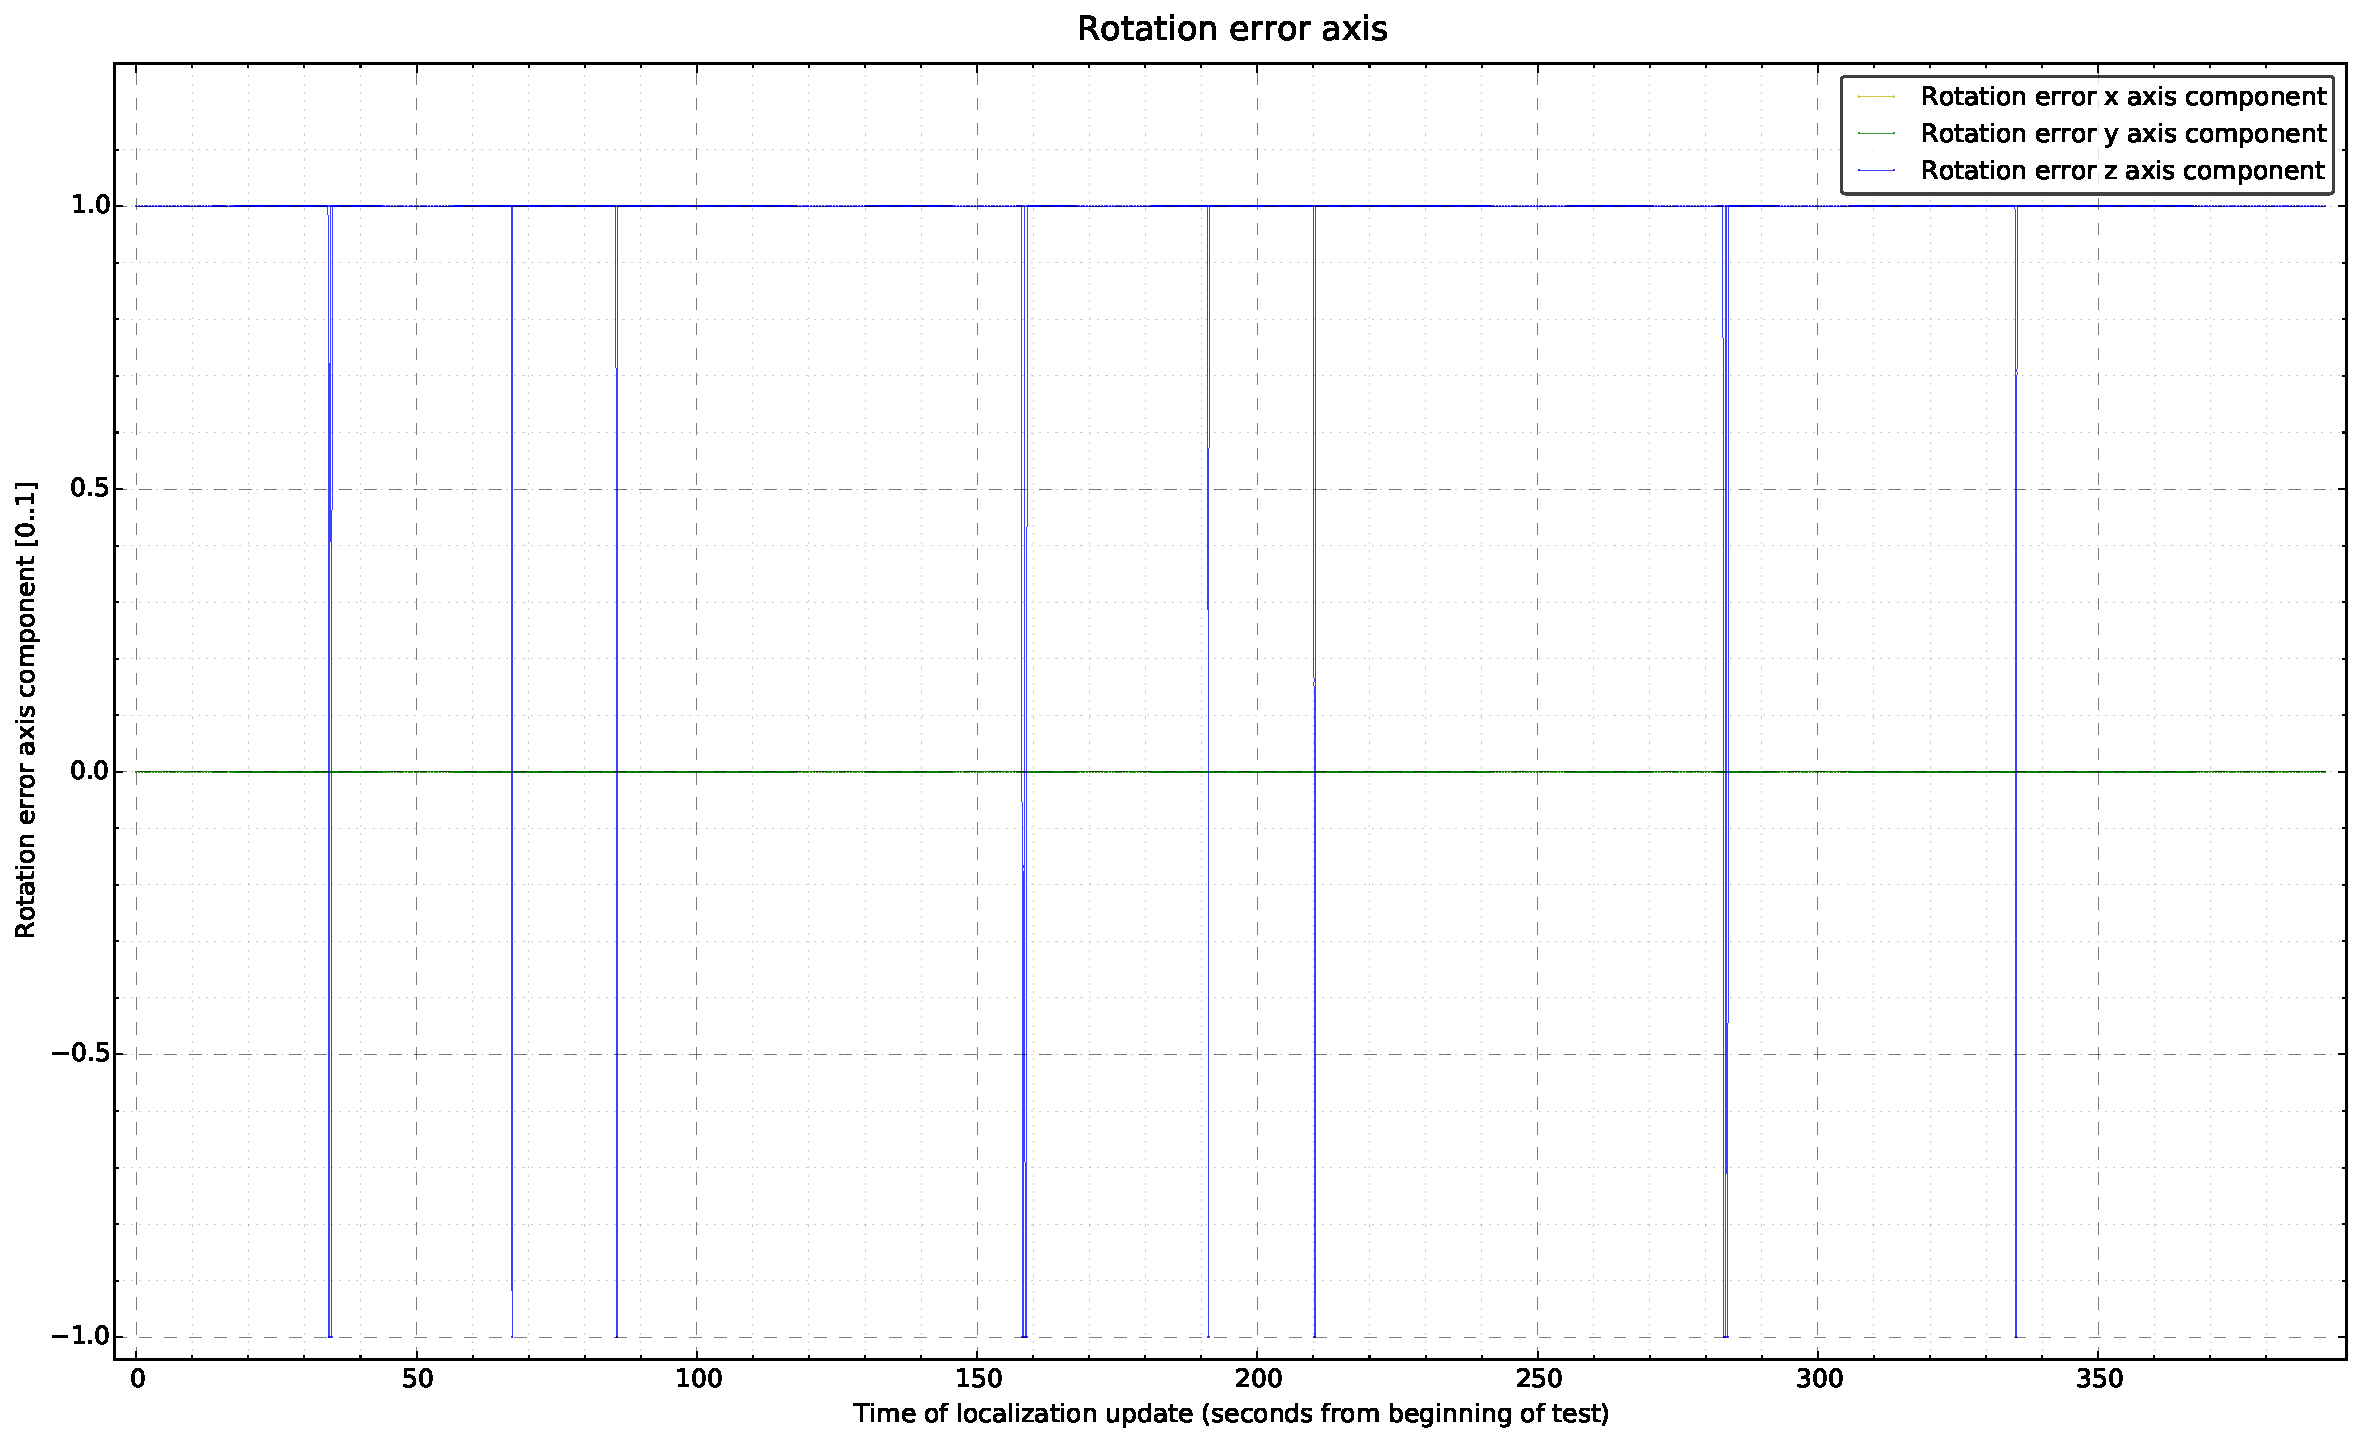
\includegraphics[width=0.69\textwidth]{appendices/tests-6dof/kinect/\currfilebase/graphs/rotation-error-axis}
	\caption{Localization system rotation errors axis}
\end{figure}


%Angular errors
\begin{figure}[H]
	\centering
	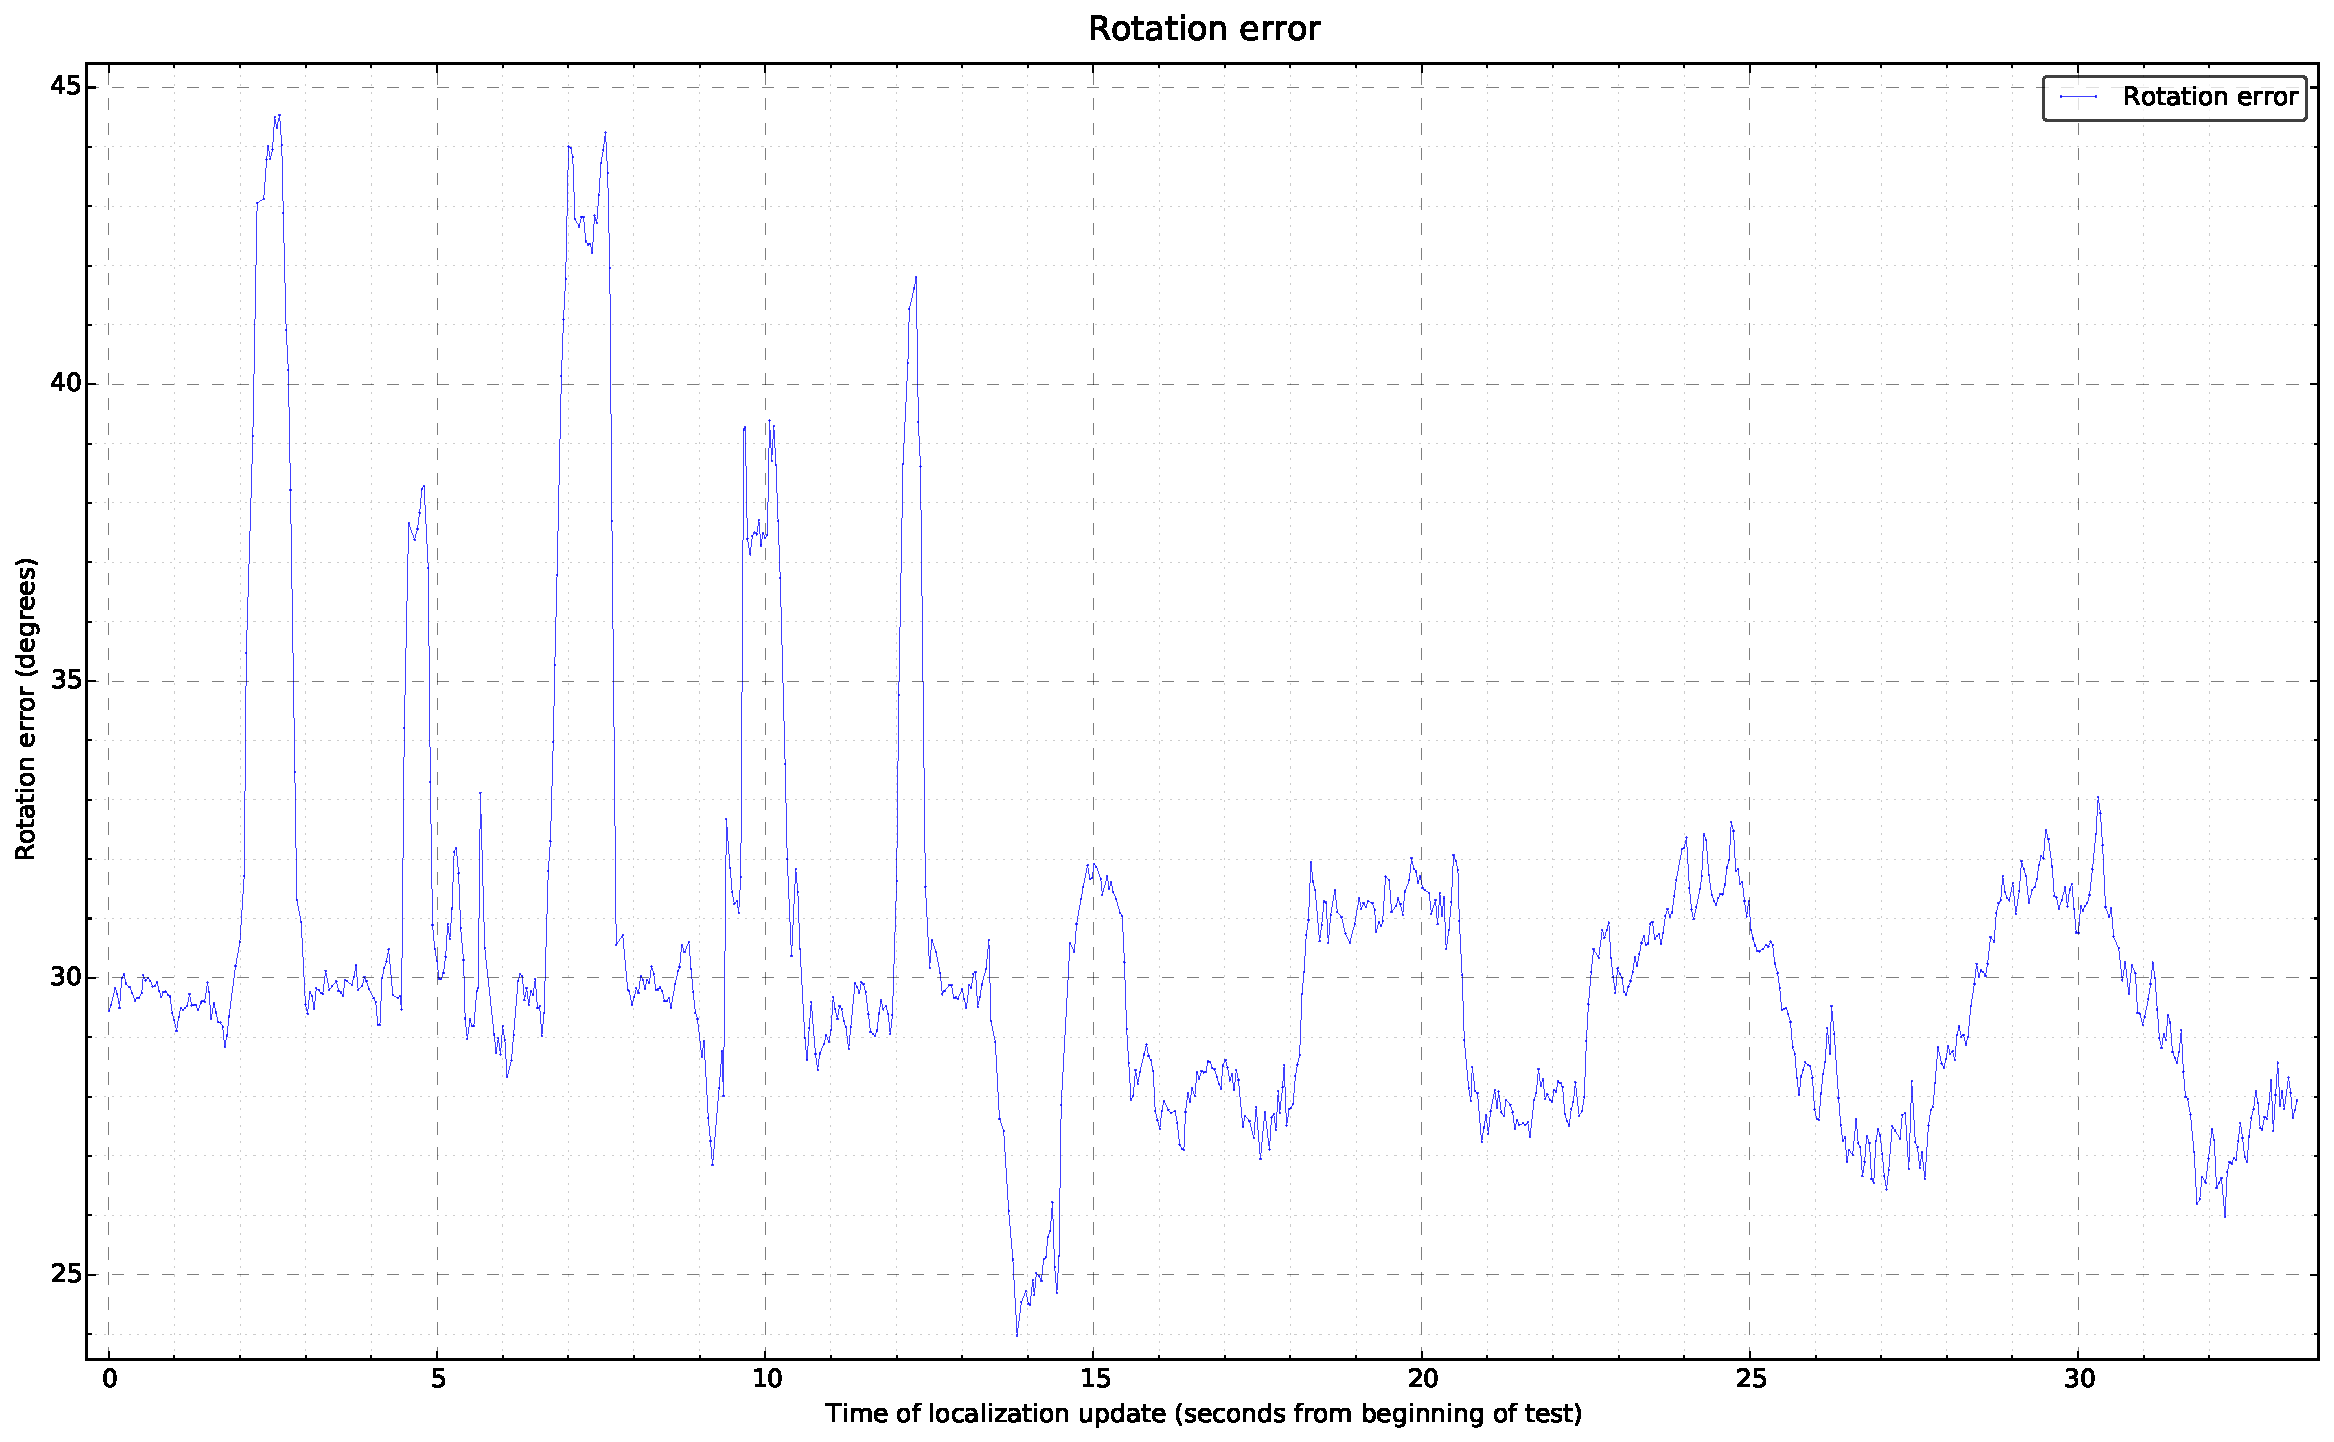
\includegraphics[width=0.69\textwidth]{appendices/tests-6dof/kinect/\currfilebase/graphs/rotation-error-degrees}
	\caption{Localization system rotation errors}
\end{figure}


%Angular errors distributions
\begin{figure}[H]
	\centering
	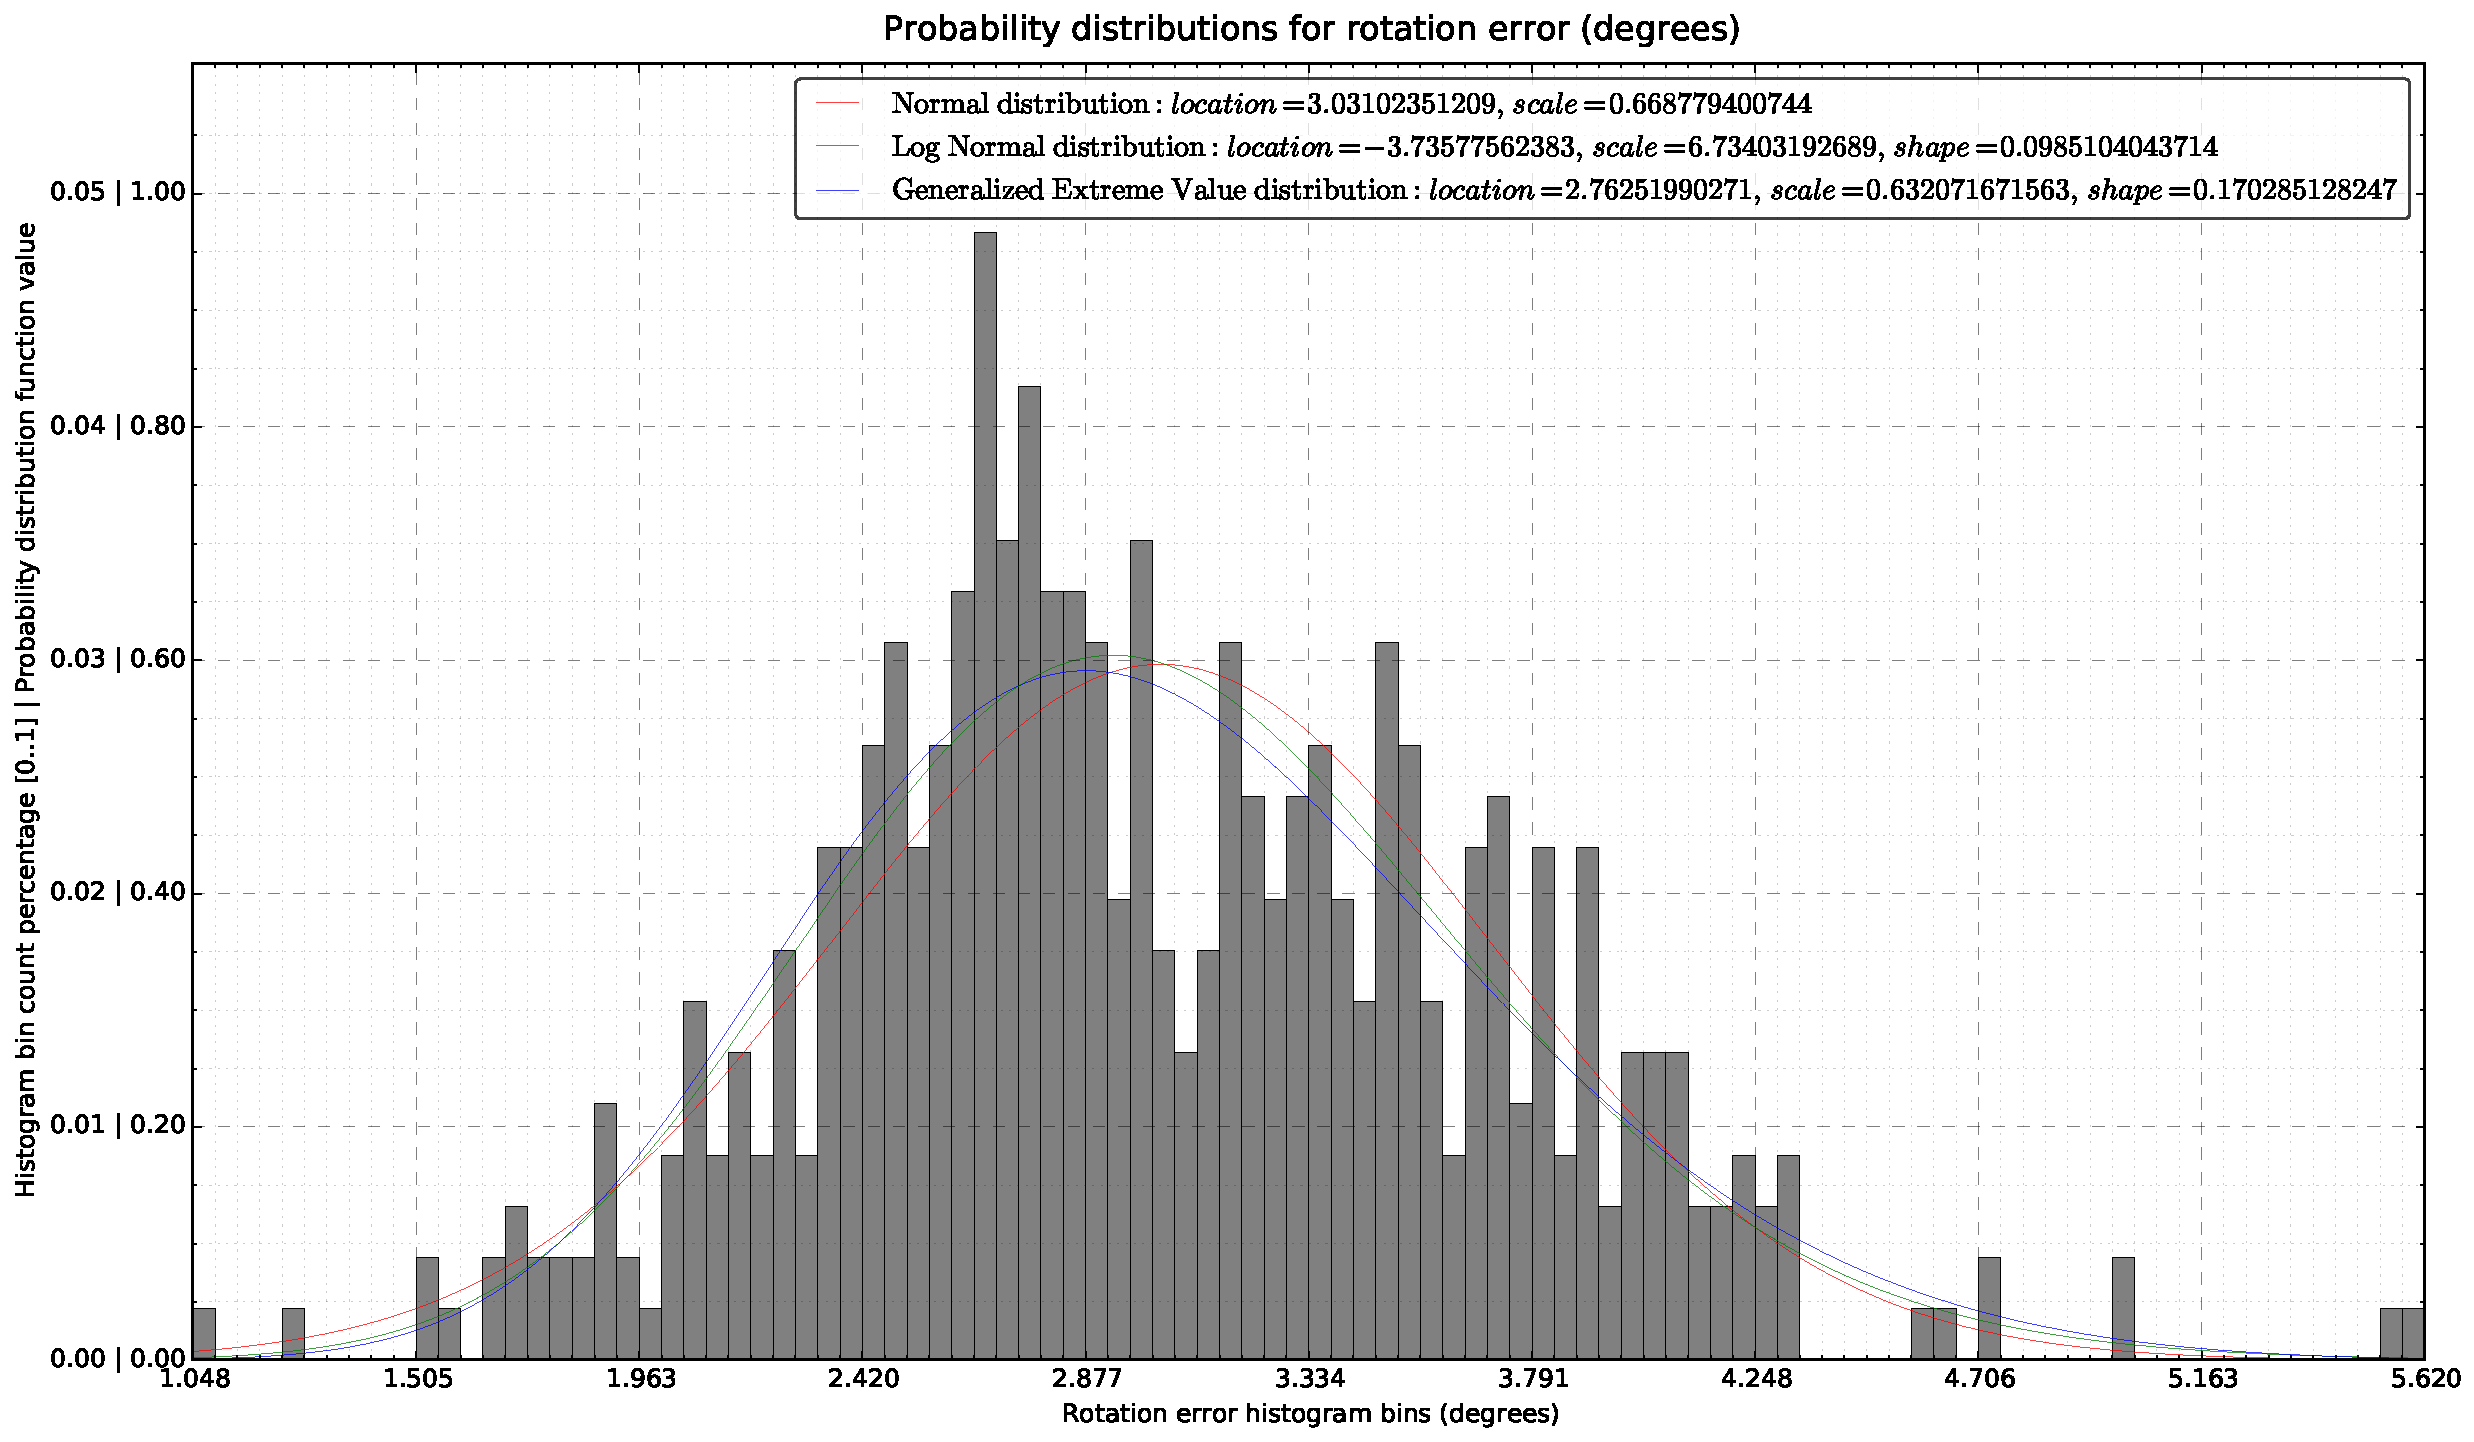
\includegraphics[width=0.73\textwidth]{appendices/tests-6dof/kinect/\currfilebase/graphs/rotation-error-degrees-distributions}
	\caption{Probability distributions for the localization system rotation errors}
\end{figure}


%Translation corrections
\begin{figure}[H]
	\centering
	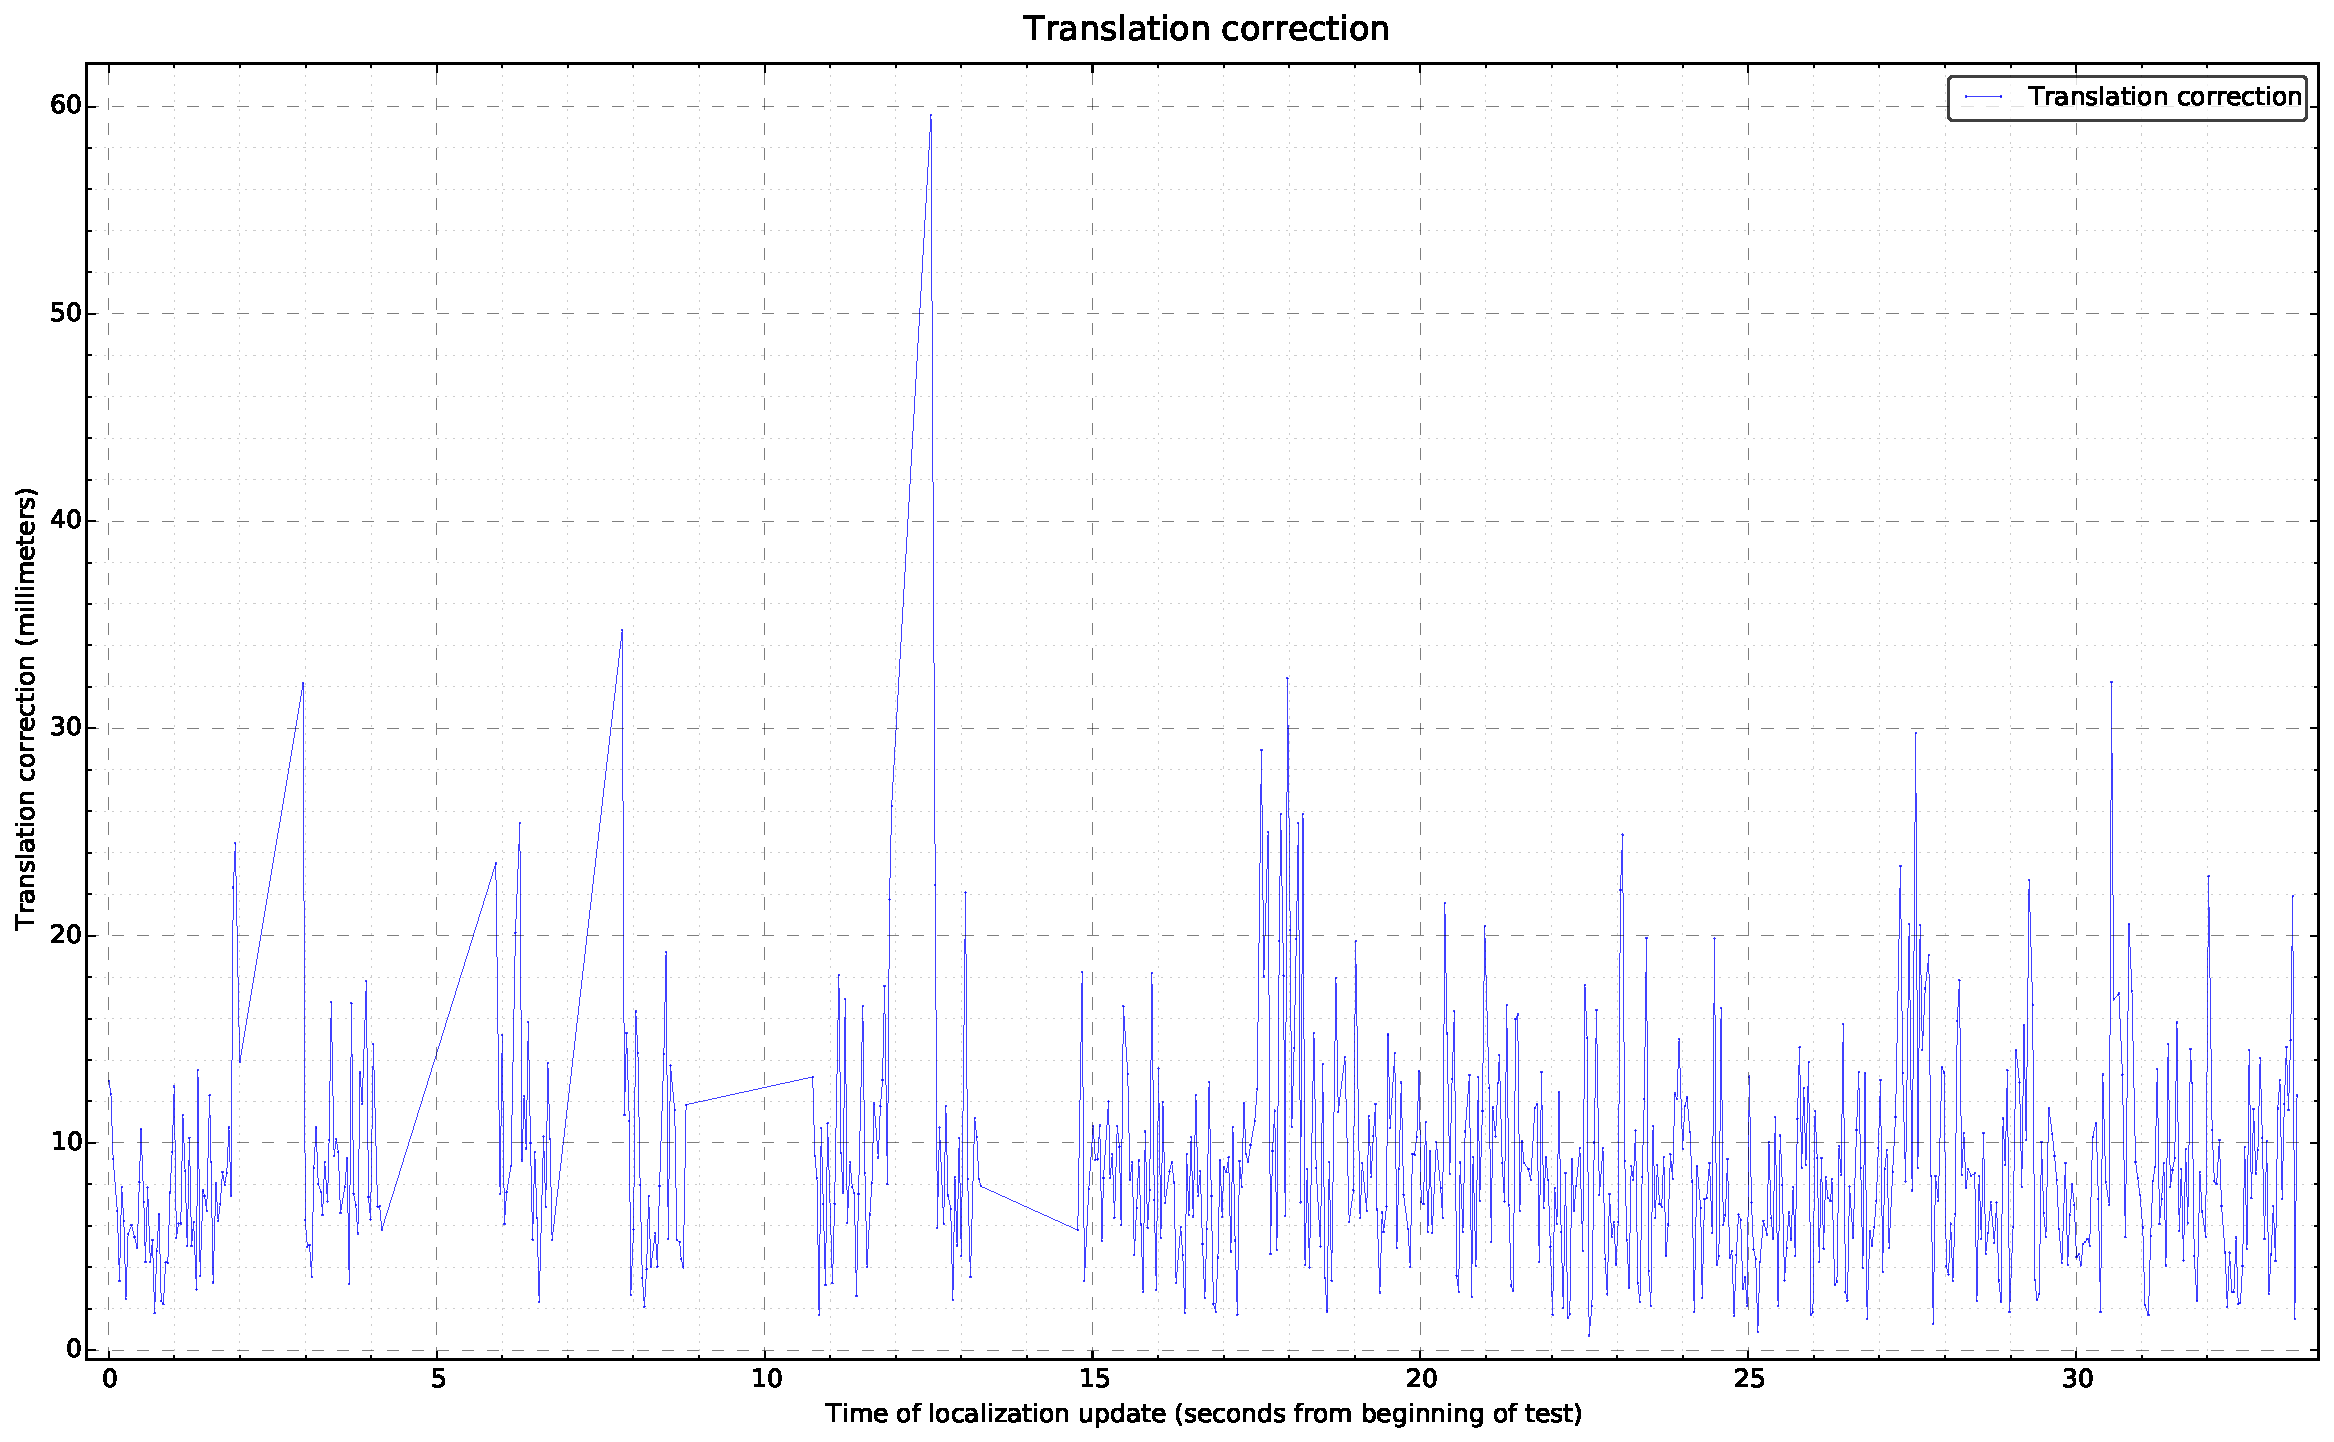
\includegraphics[width=0.69\textwidth]{appendices/tests-6dof/kinect/\currfilebase/graphs/translation-correction-millimeters}
	\caption{Translation corrections performed by the localization system}
\end{figure}

\begin{figure}[H]
	\centering
	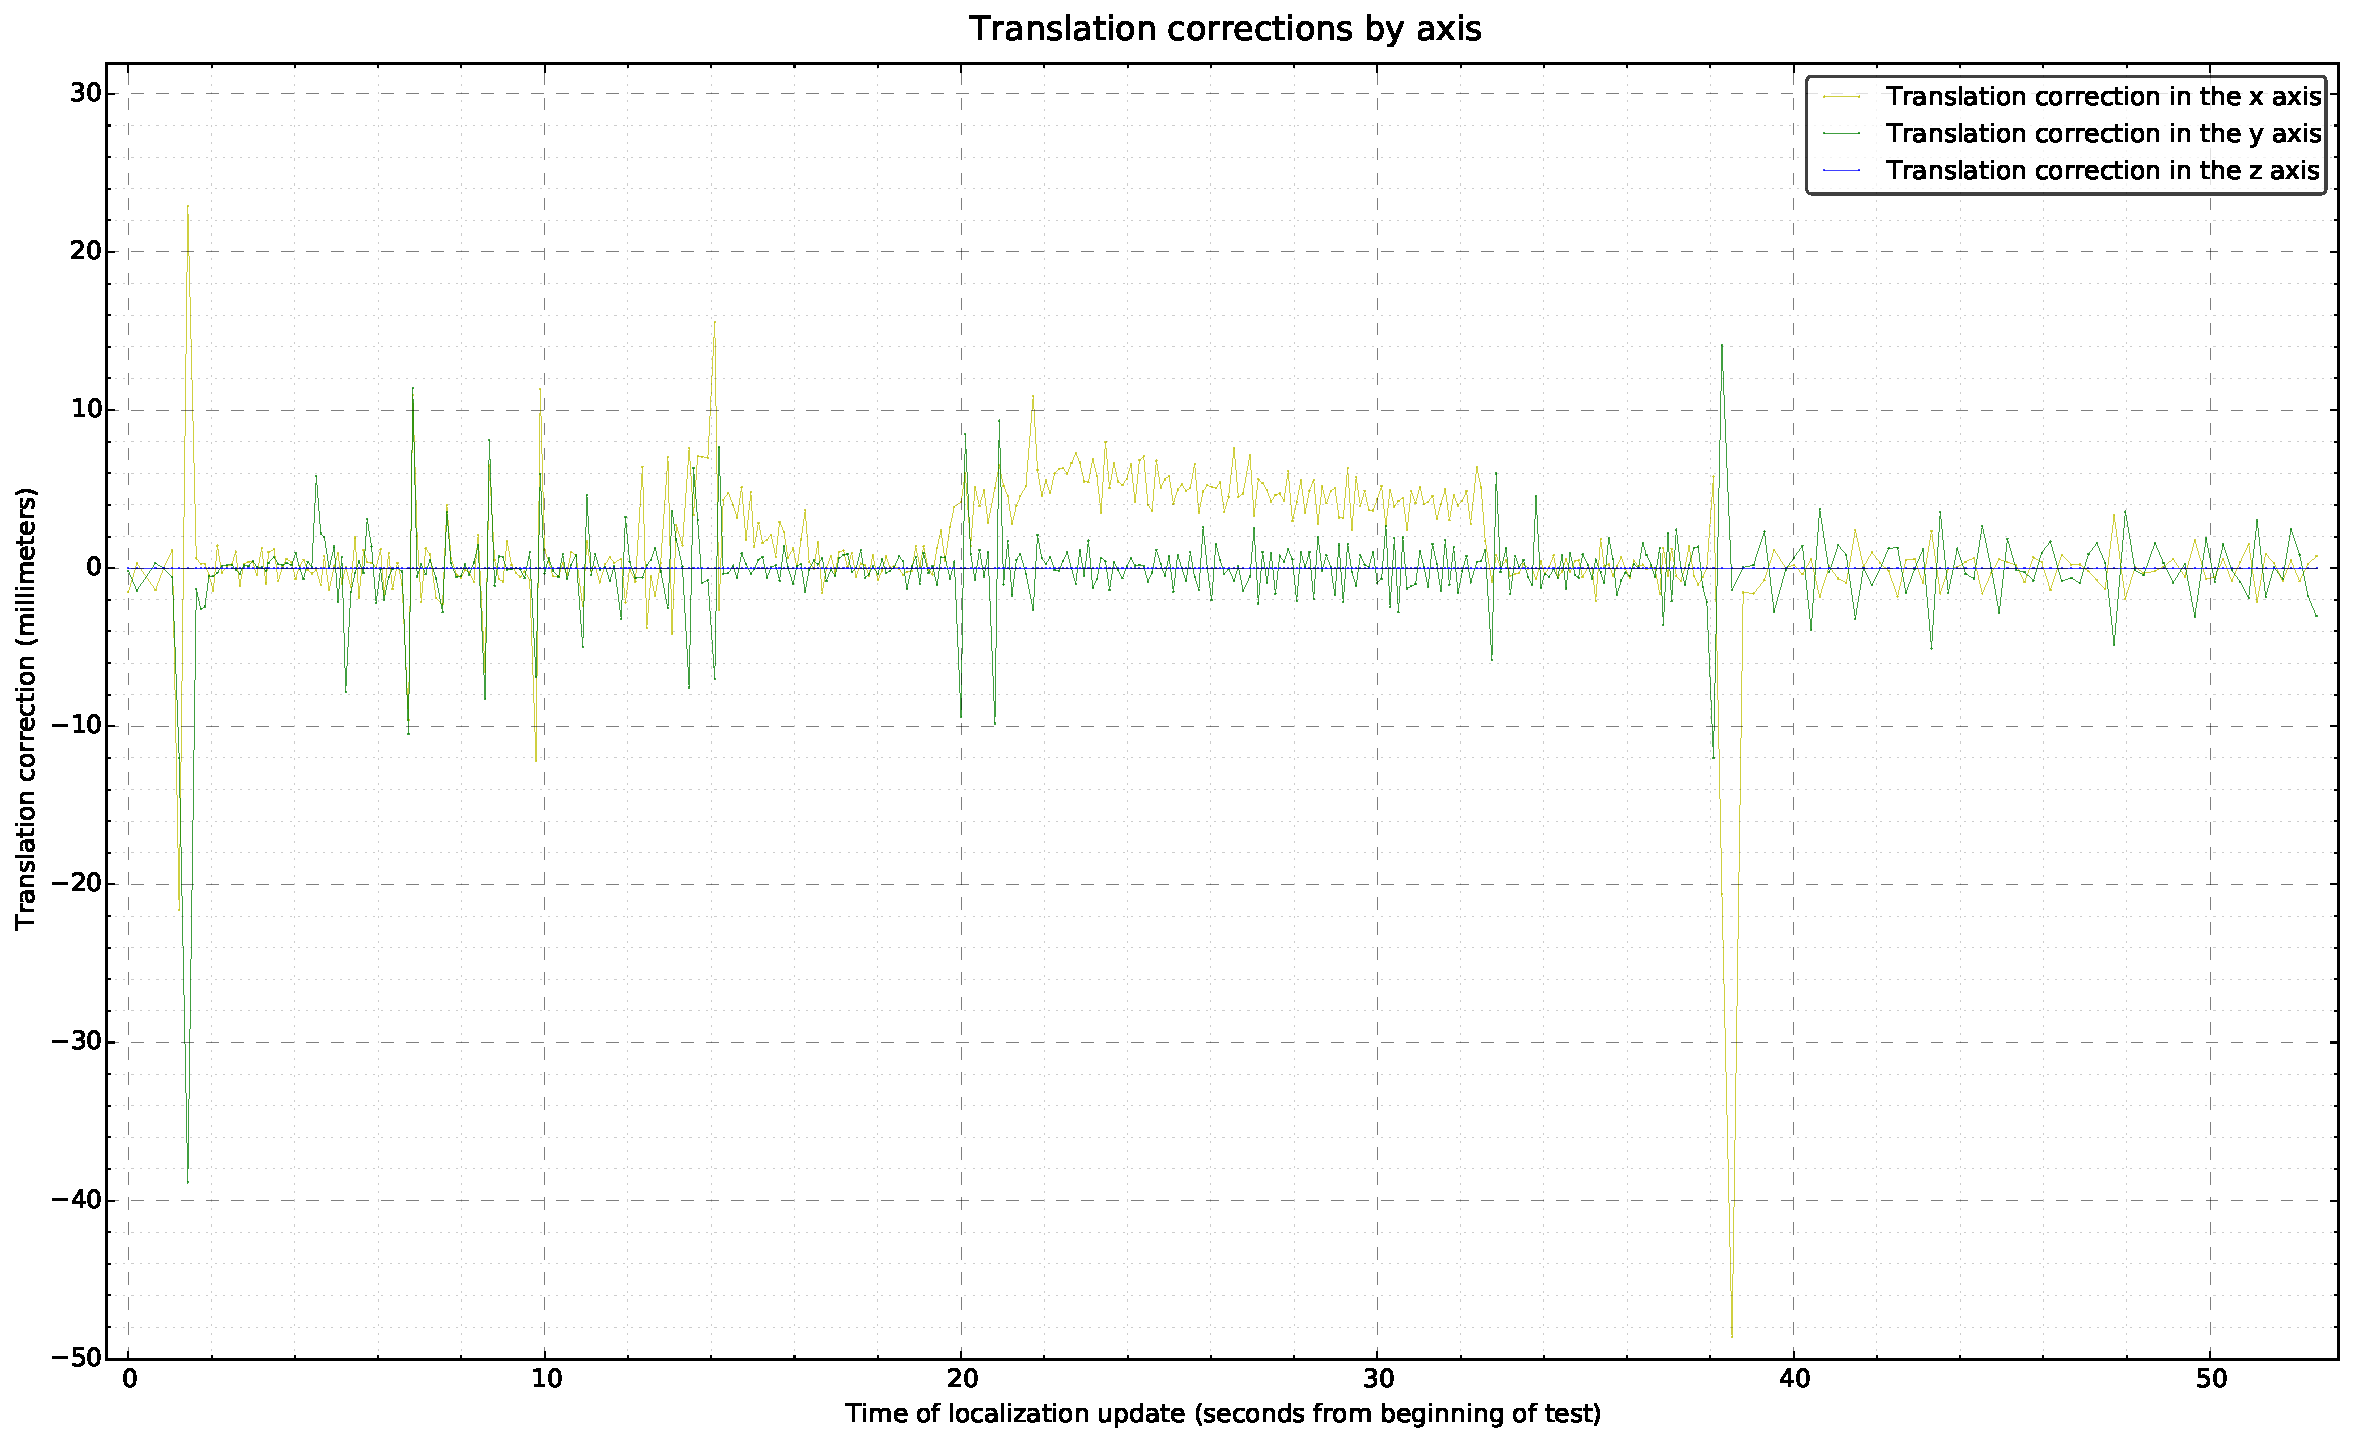
\includegraphics[width=0.69\textwidth]{appendices/tests-6dof/kinect/\currfilebase/graphs/translation-corrections-components-millimeters}
	\caption{Translation corrections components performed by the localization system}
\end{figure}

\begin{figure}[H]
	\centering
	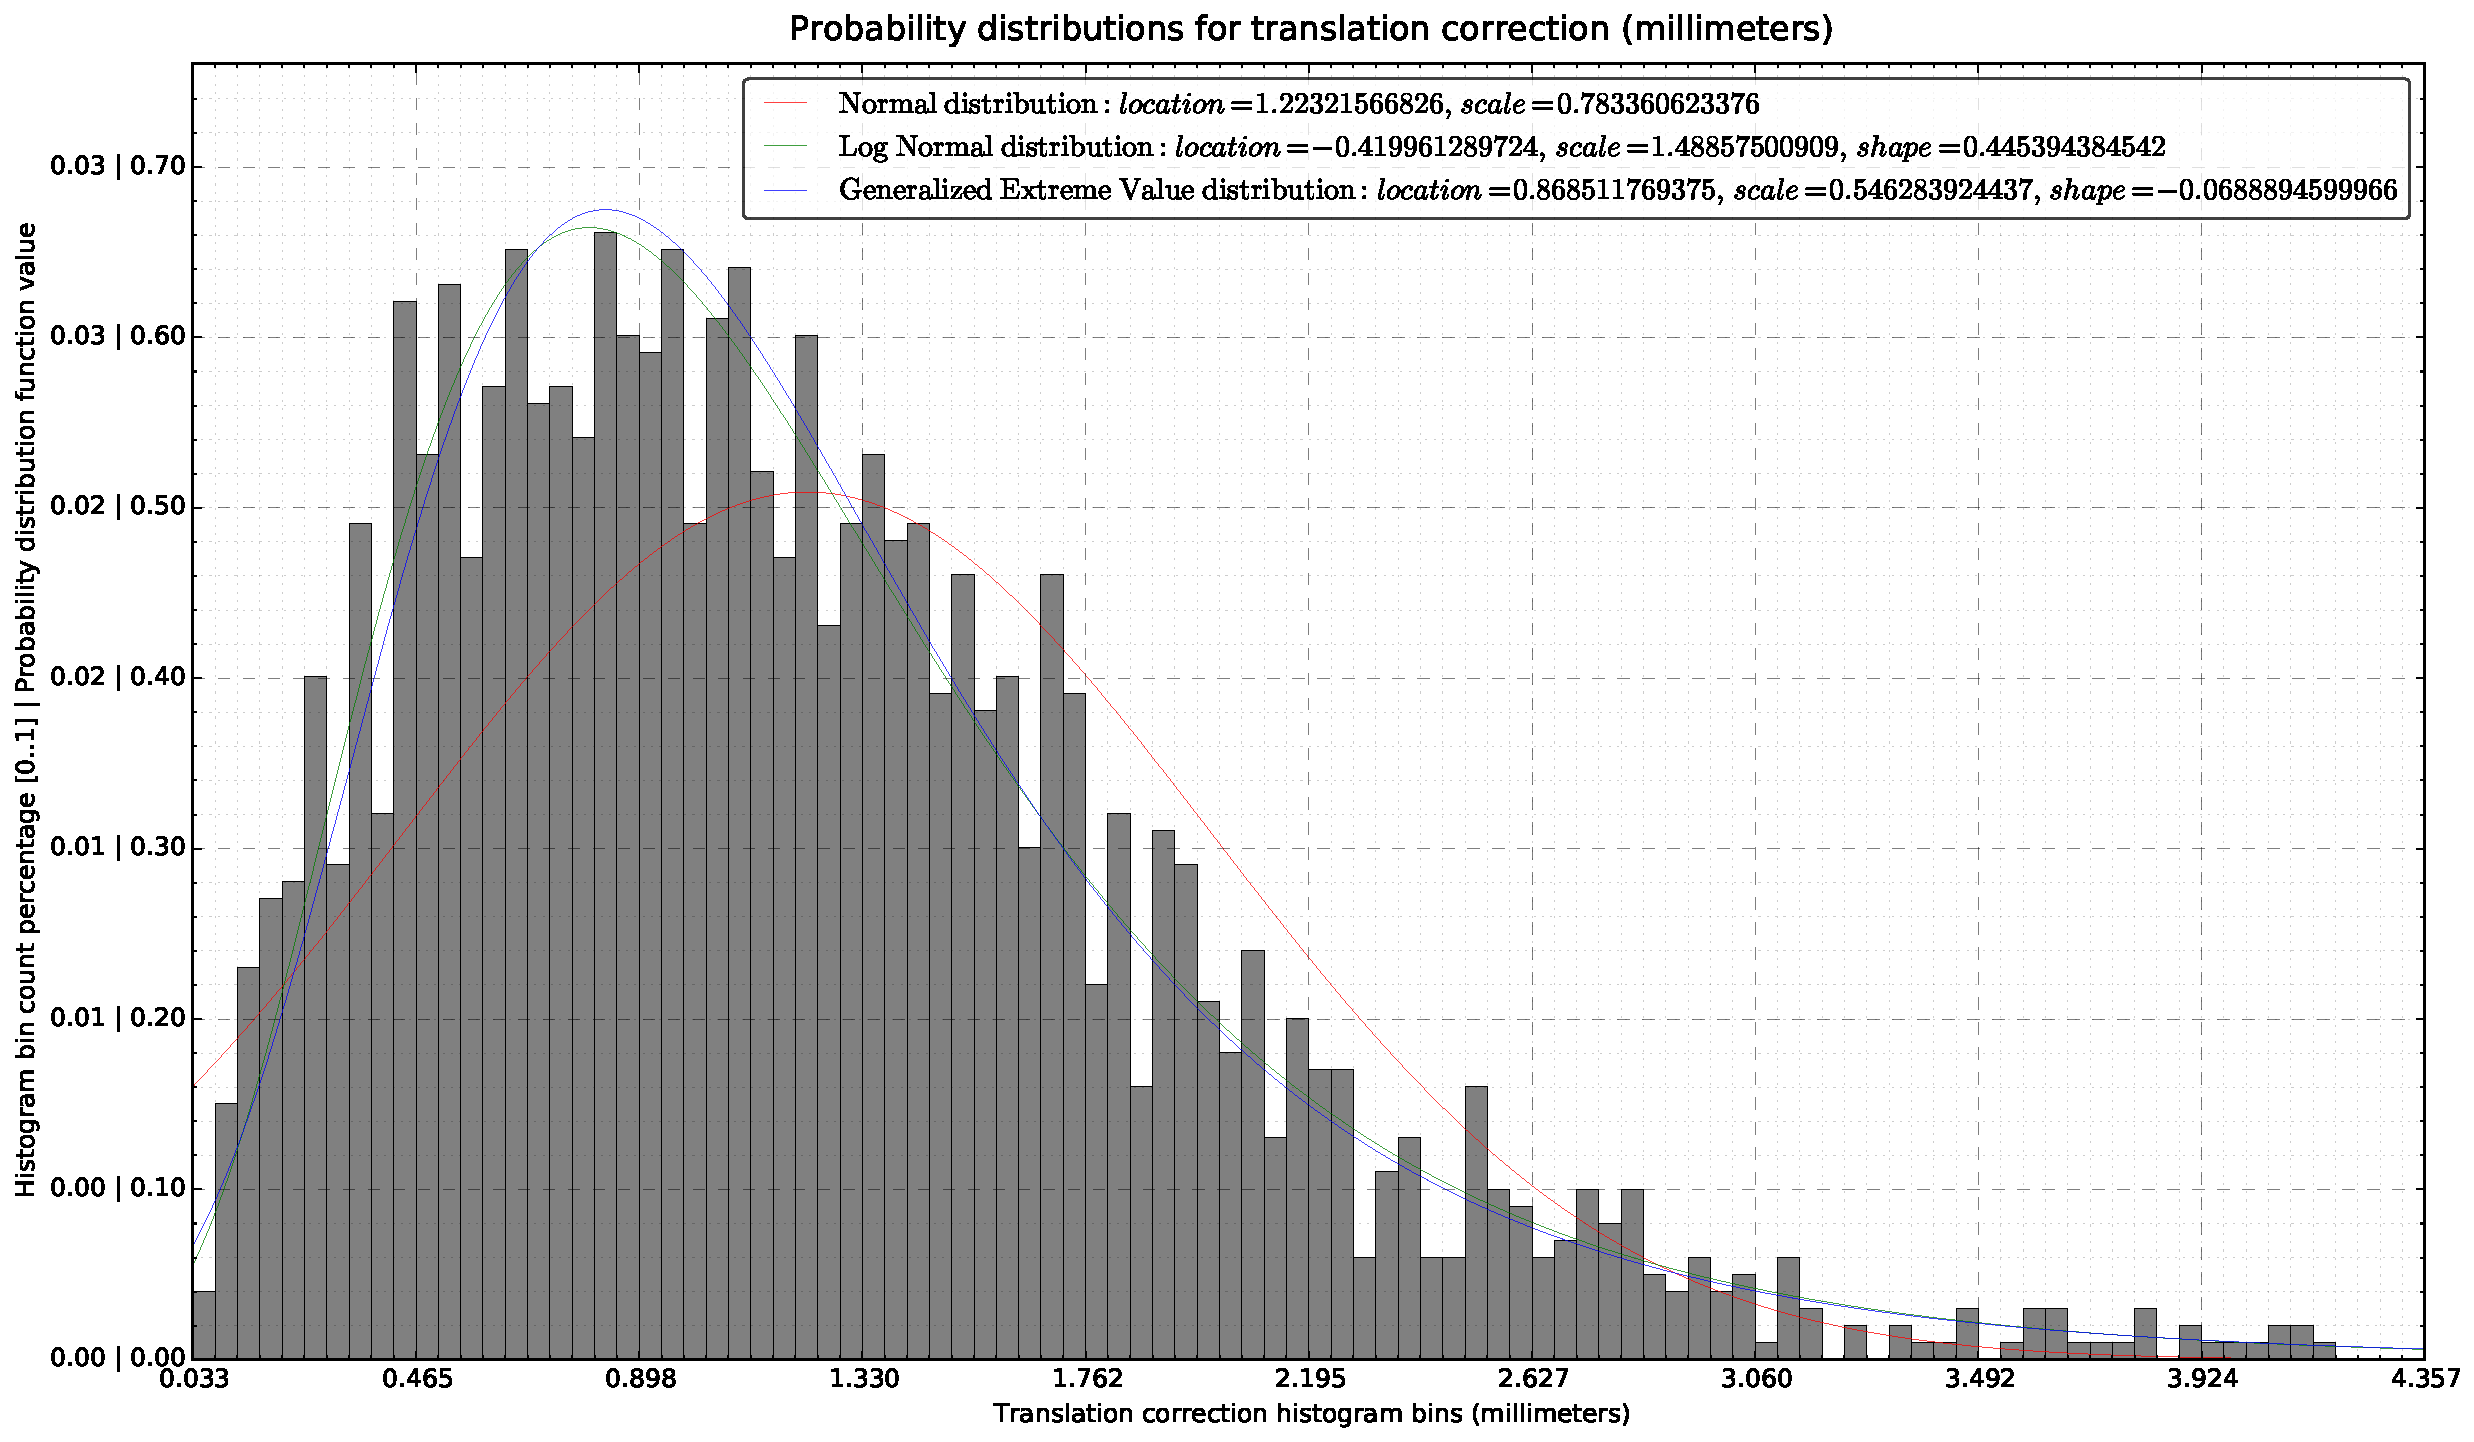
\includegraphics[width=0.69\textwidth]{appendices/tests-6dof/kinect/\currfilebase/graphs/translation-correction-millimeters-distributions}
	\caption{Probability distributions for the translation corrections performed by the localization system}
\end{figure}


%Rotation corrections axis
\begin{figure}[H]
	\centering
	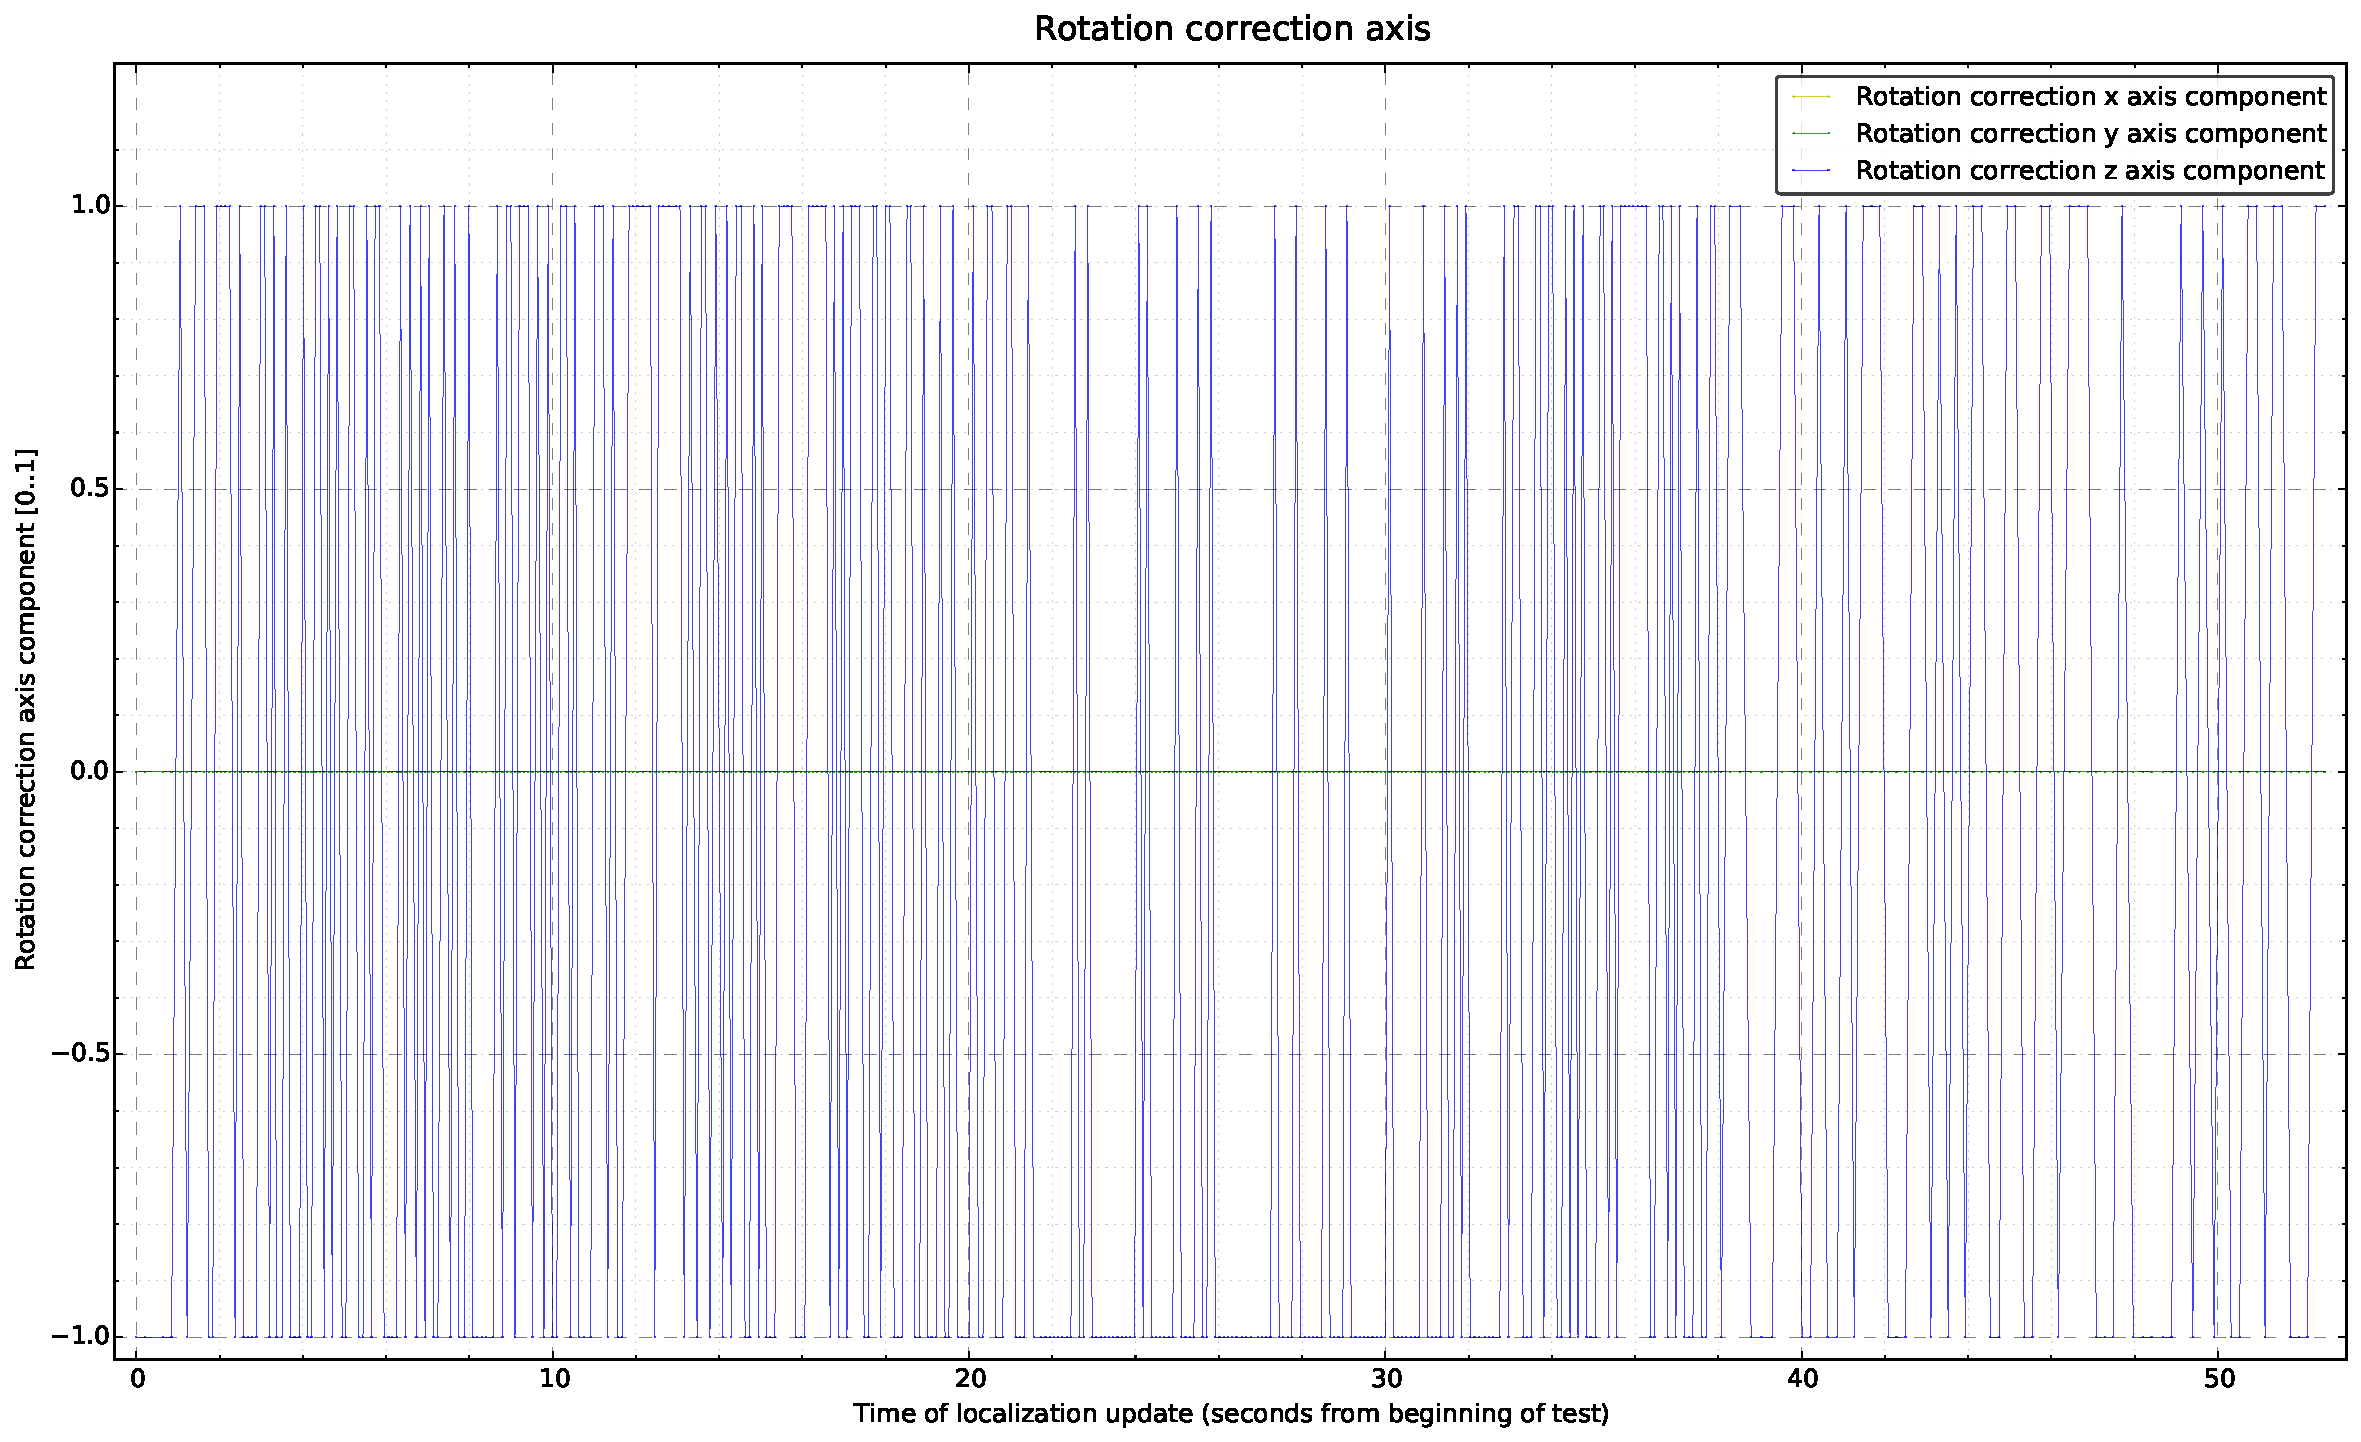
\includegraphics[width=0.69\textwidth]{appendices/tests-6dof/kinect/\currfilebase/graphs/rotation-correction-axis}
	\caption{Rotation corrections (axis) performed by the localization system}
\end{figure}

\begin{figure}[H]
	\centering
	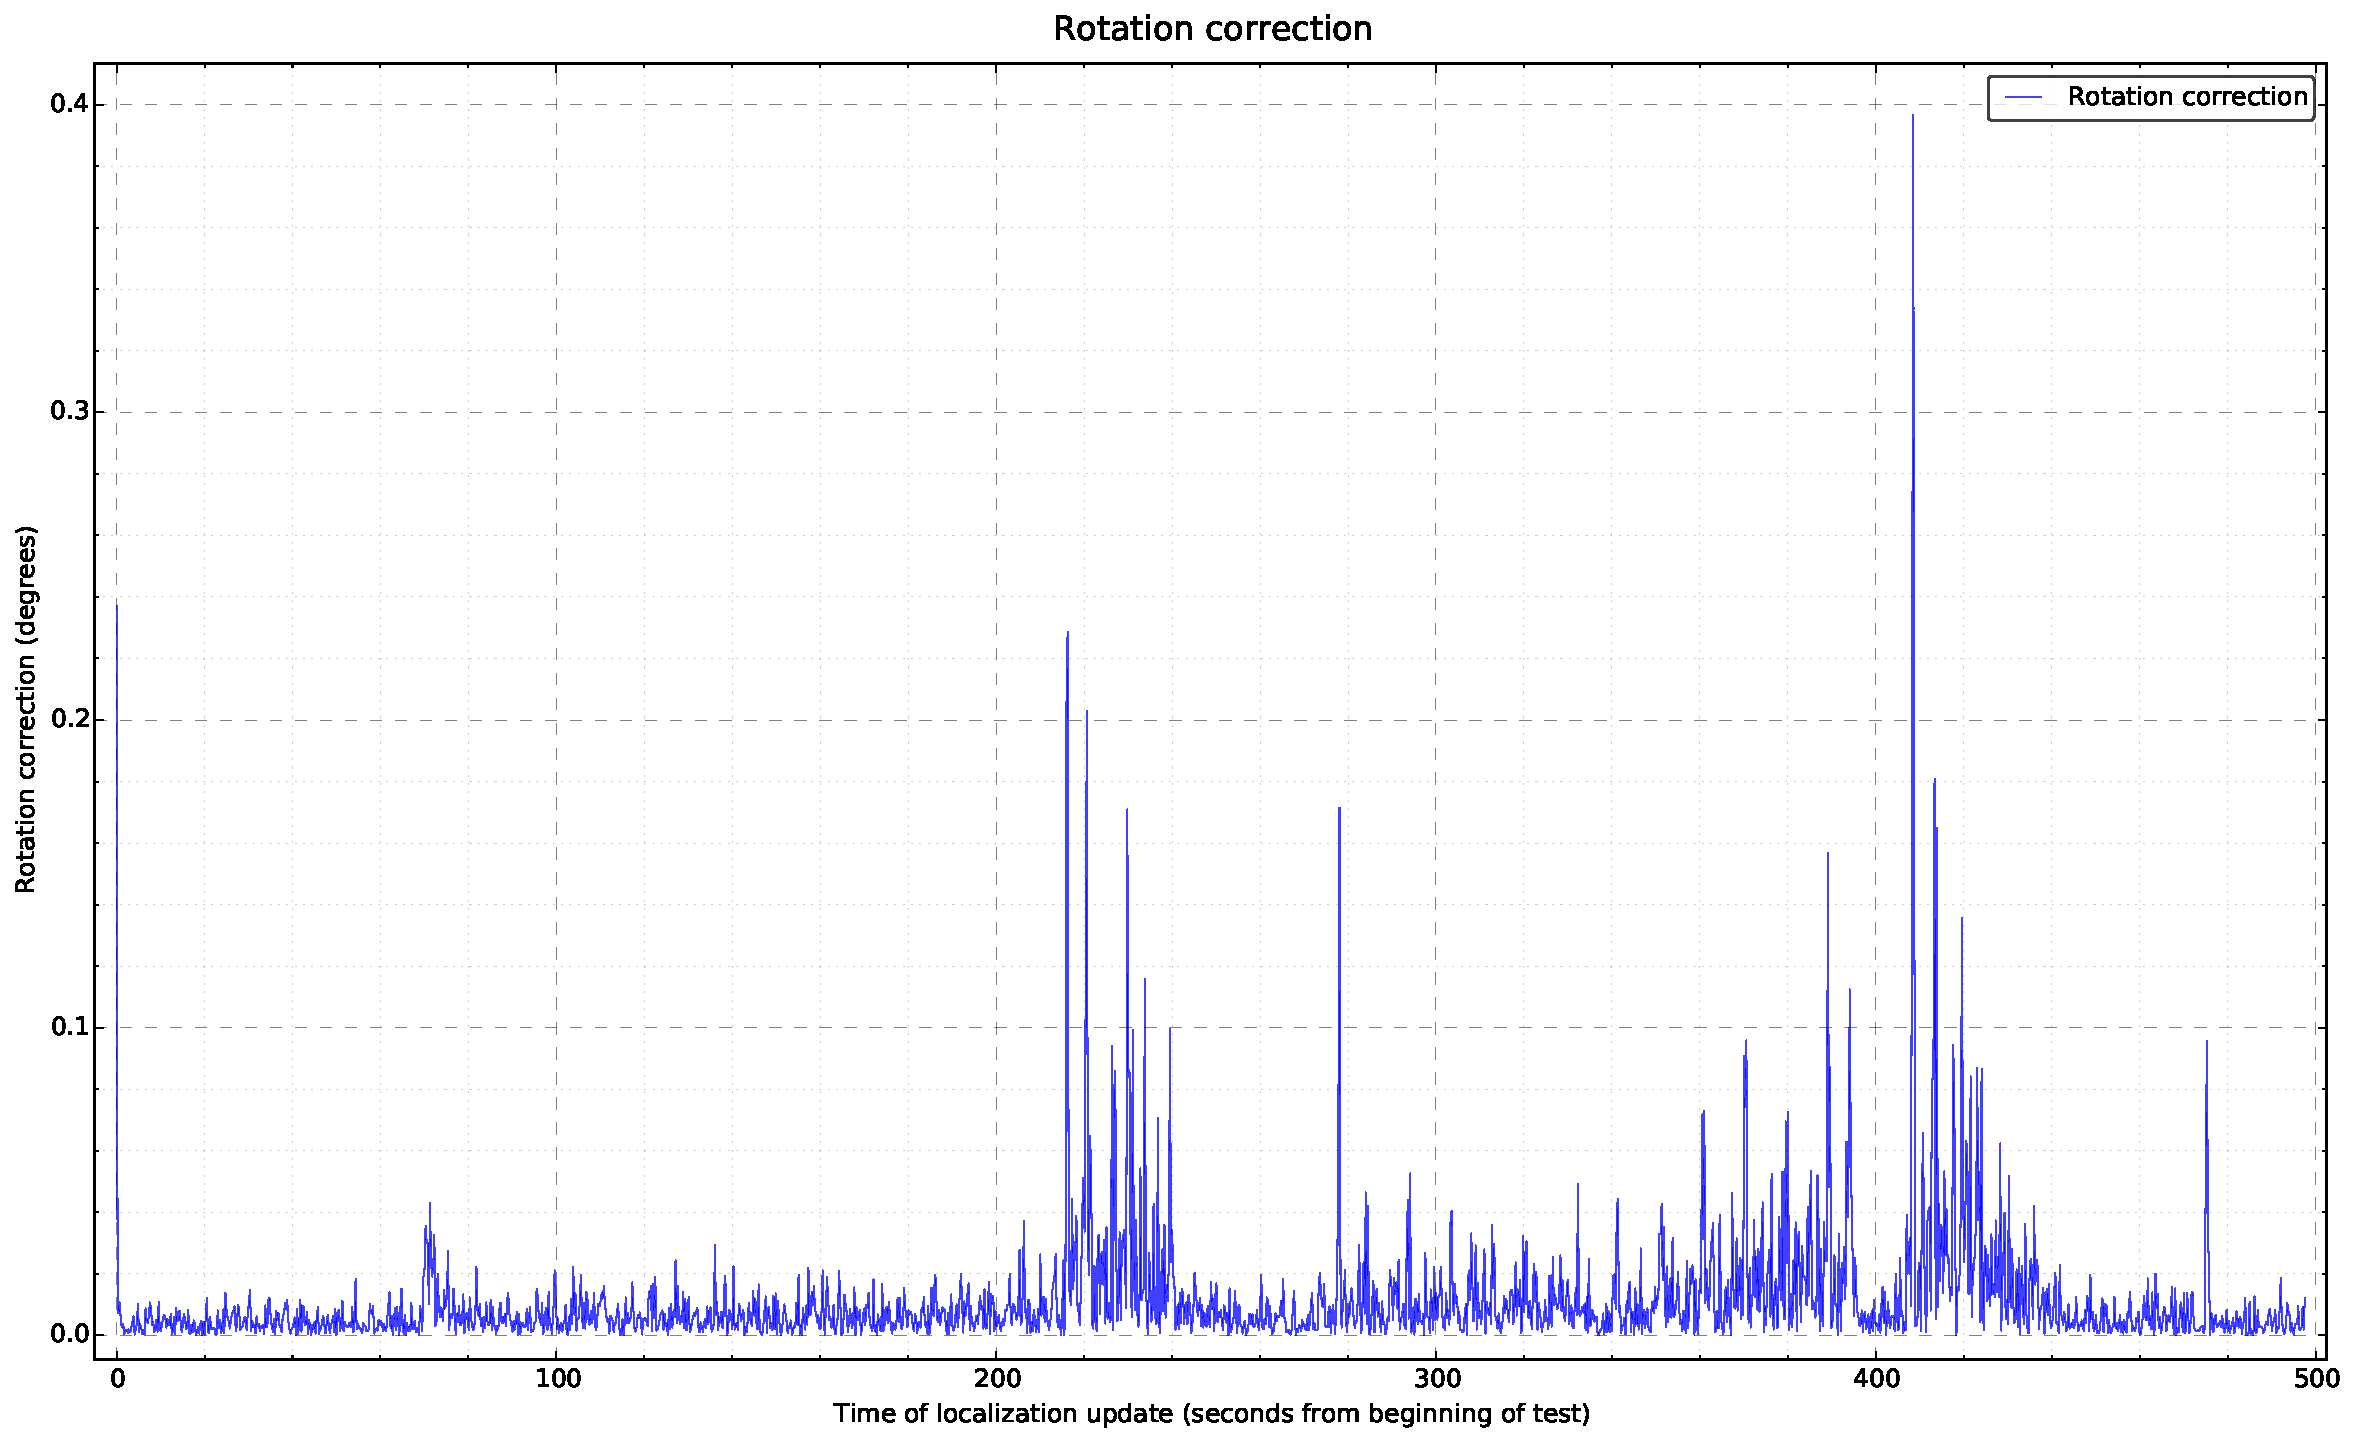
\includegraphics[width=0.69\textwidth]{appendices/tests-6dof/kinect/\currfilebase/graphs/rotation-correction-degrees}
	\caption{Rotation corrections performed by the localization system}
\end{figure}

\begin{figure}[H]
	\centering
	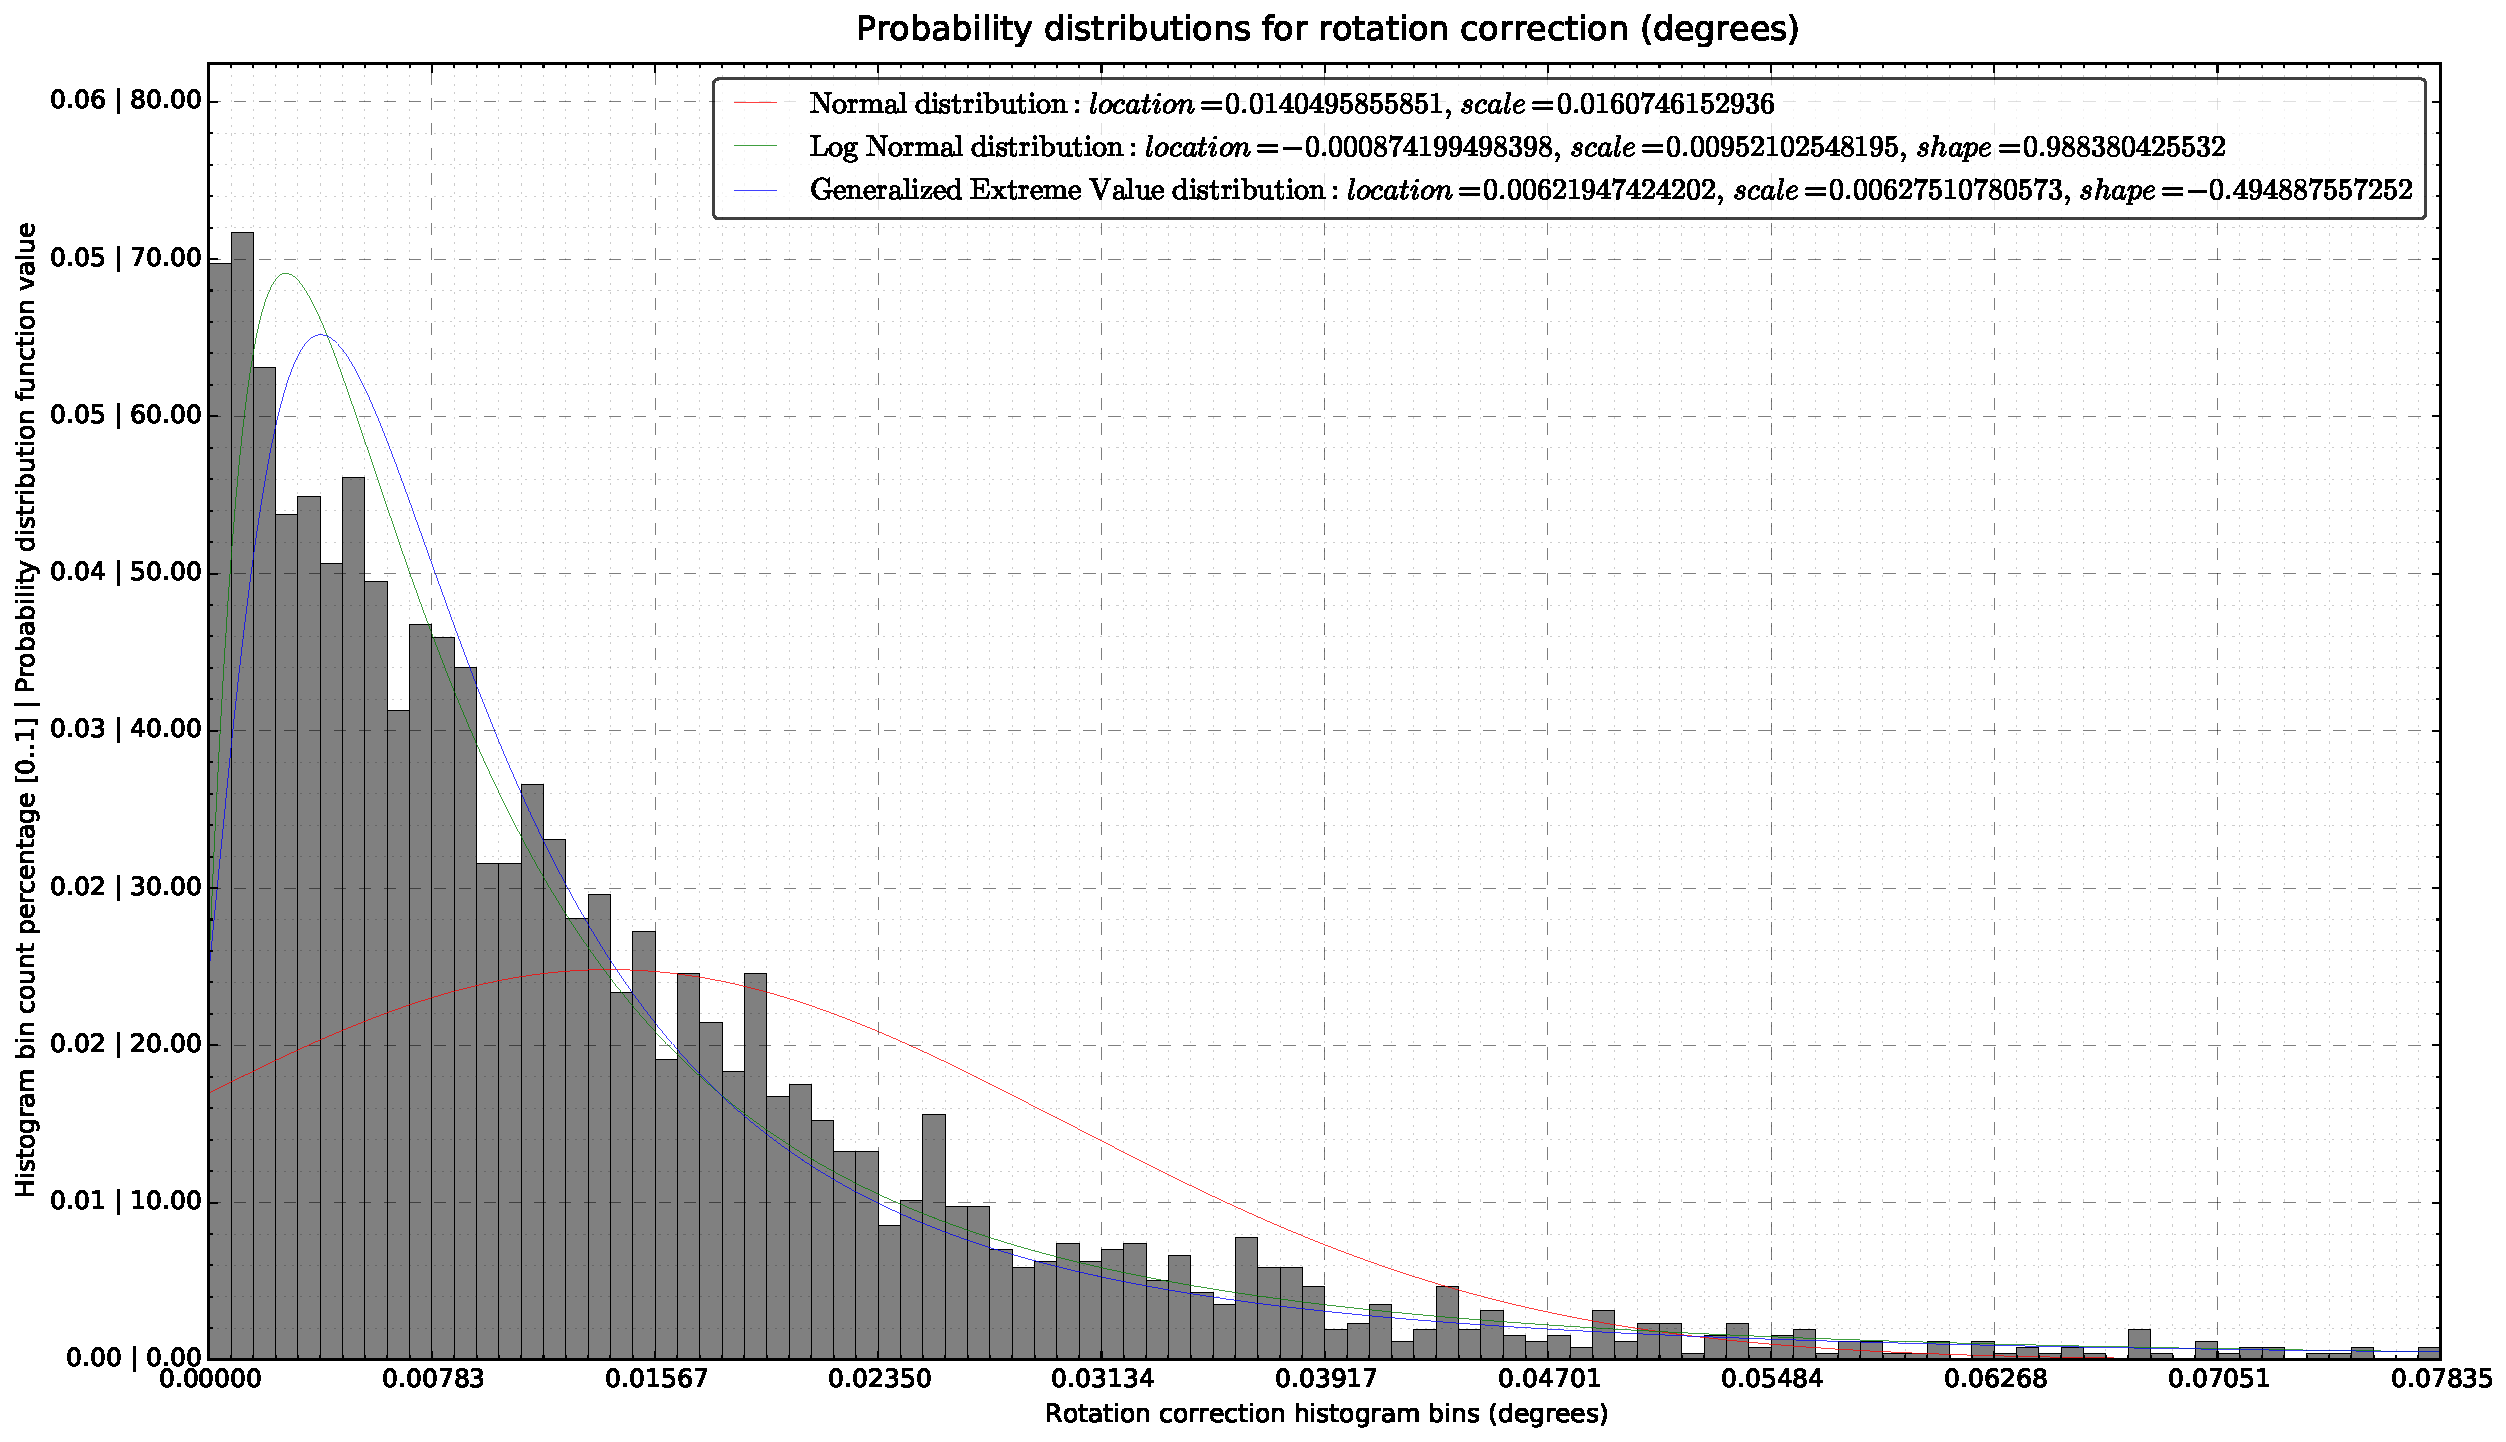
\includegraphics[width=0.69\textwidth]{appendices/tests-6dof/kinect/\currfilebase/graphs/rotation-correction-degrees-distributions}
	\caption{Probability distributions for the rotation corrections performed by the localization system}
\end{figure}


%Registered points (inliers / outliers)
\begin{figure}[H]
	\centering
	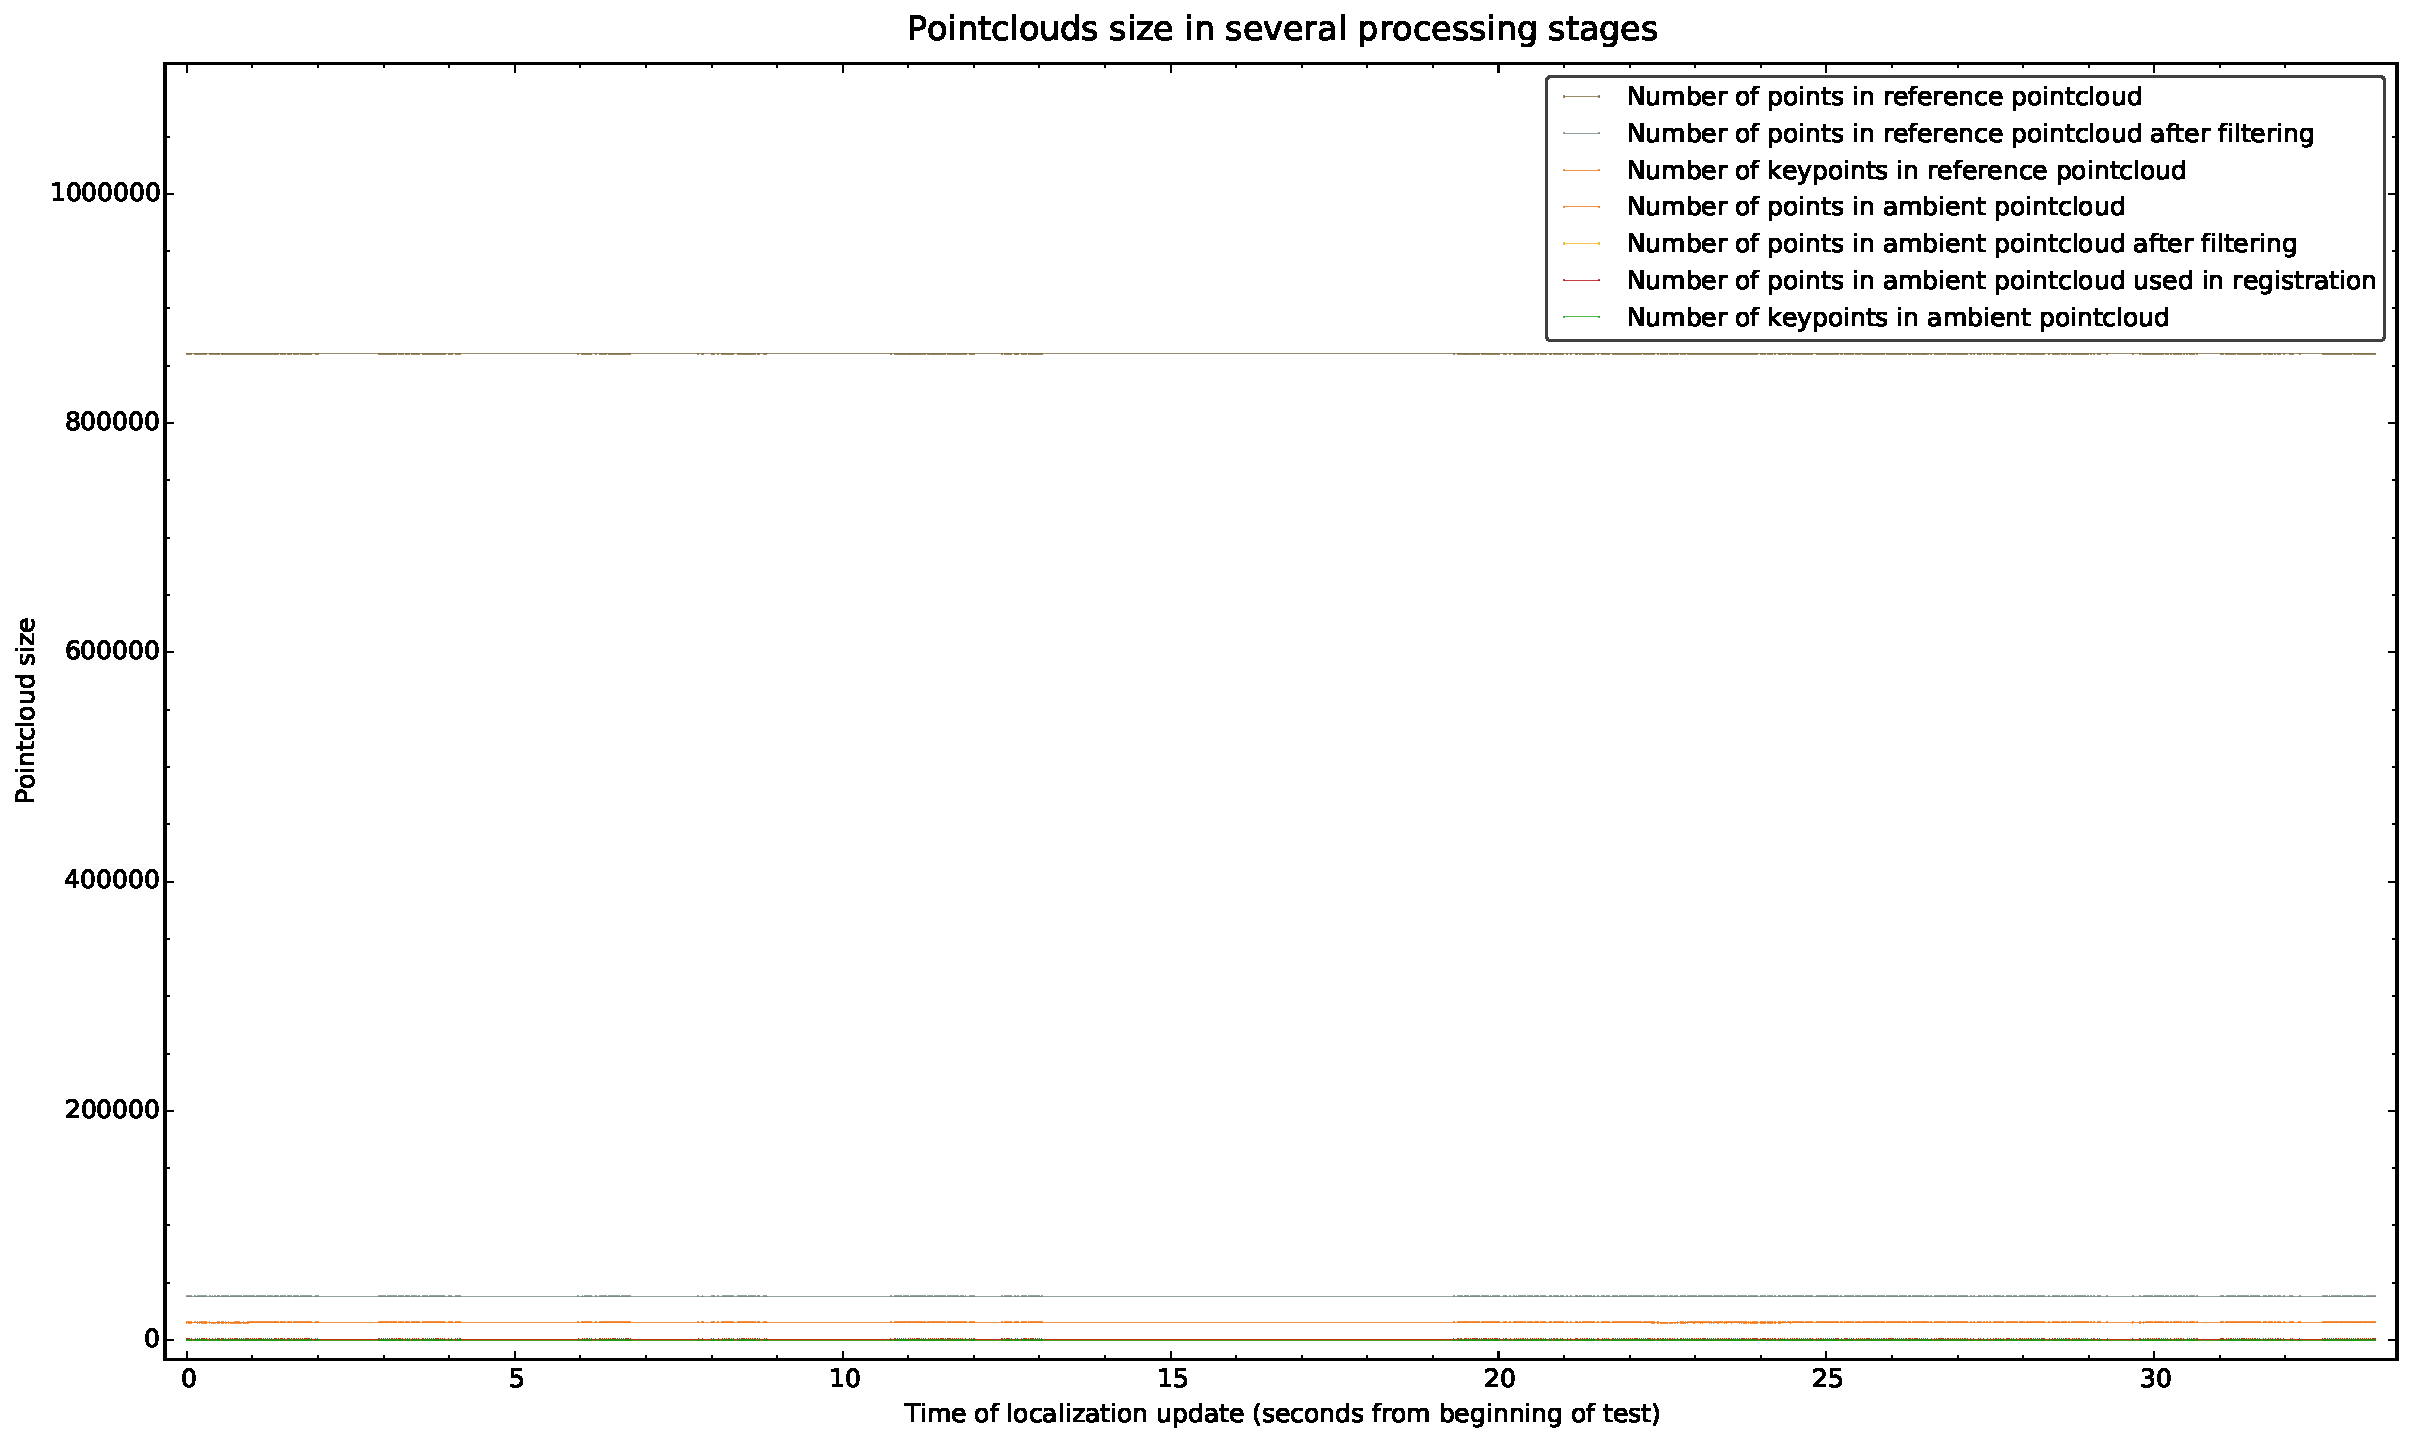
\includegraphics[width=0.69\textwidth]{appendices/tests-6dof/kinect/\currfilebase/graphs/pointclouds-size}
	\caption{Point clouds size in several of the localization system processing stages}
\end{figure}

\begin{figure}[H]
	\centering
	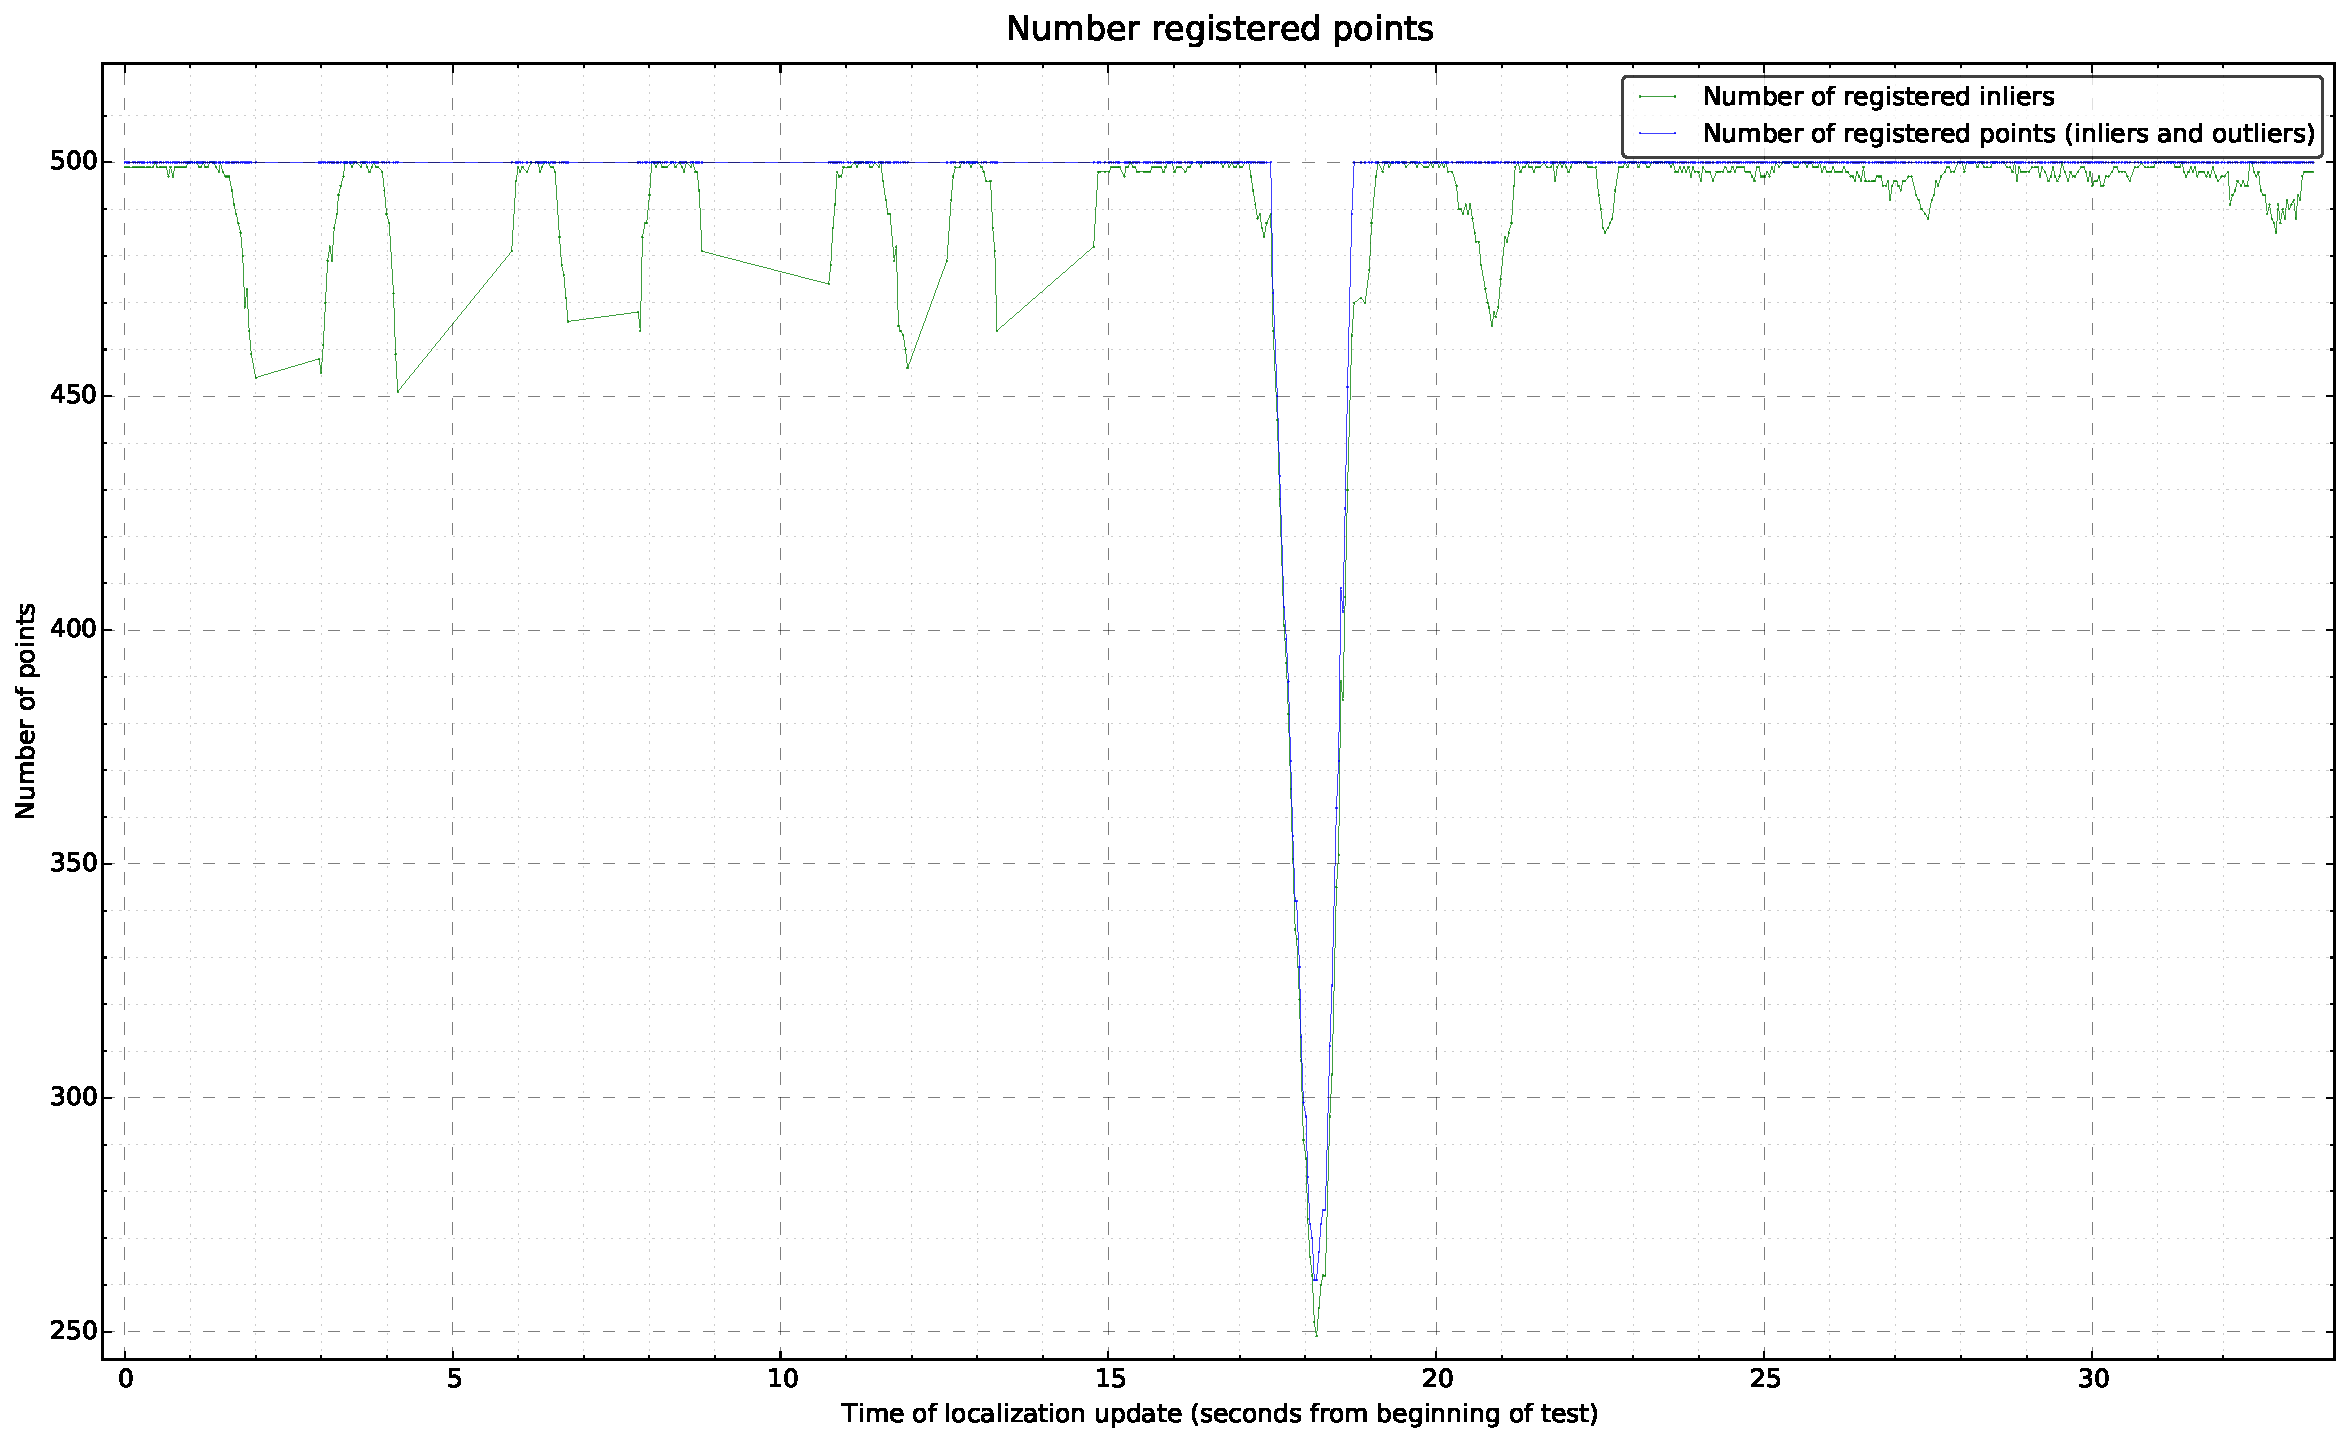
\includegraphics[width=0.69\textwidth]{appendices/tests-6dof/kinect/\currfilebase/graphs/registered-points}
	\caption{Number of registered points}
\end{figure}

\begin{figure}[H]
	\centering
	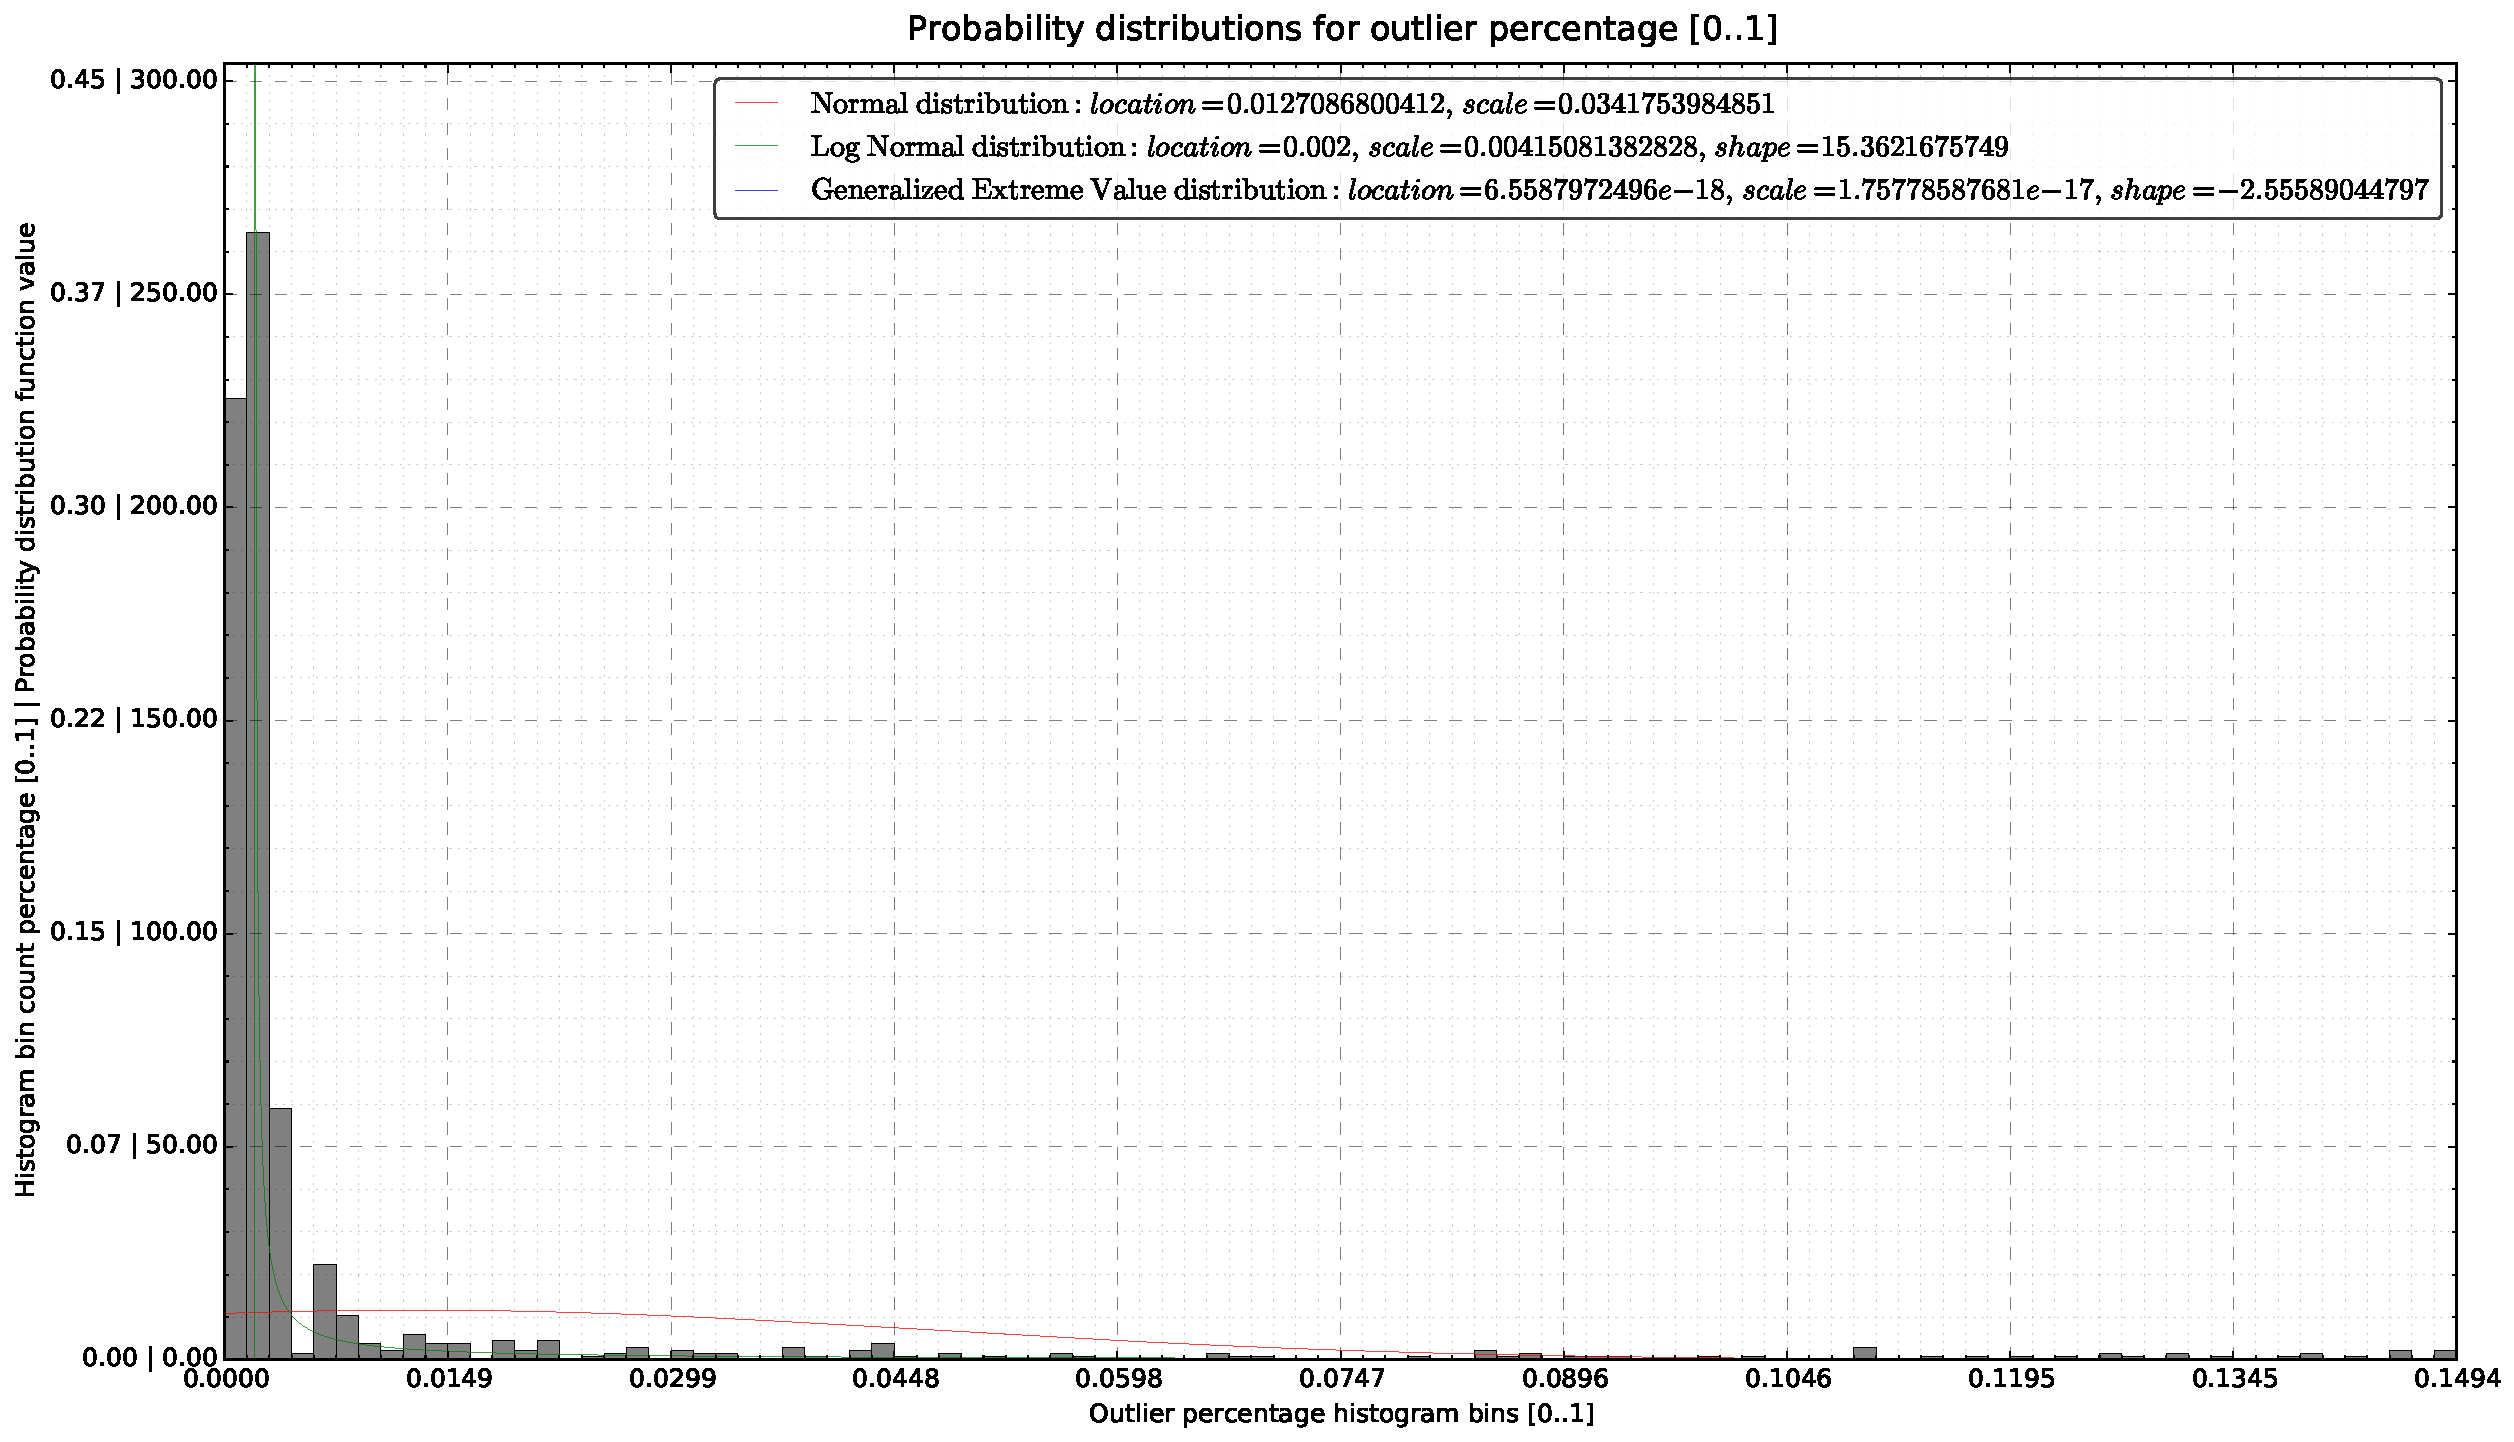
\includegraphics[width=0.69\textwidth]{appendices/tests-6dof/kinect/\currfilebase/graphs/outlier-percentage-distributions}
	\caption{Probability distributions for the ambient point cloud outlier percentage}
\end{figure}


\begin{figure}[H]
	\centering
	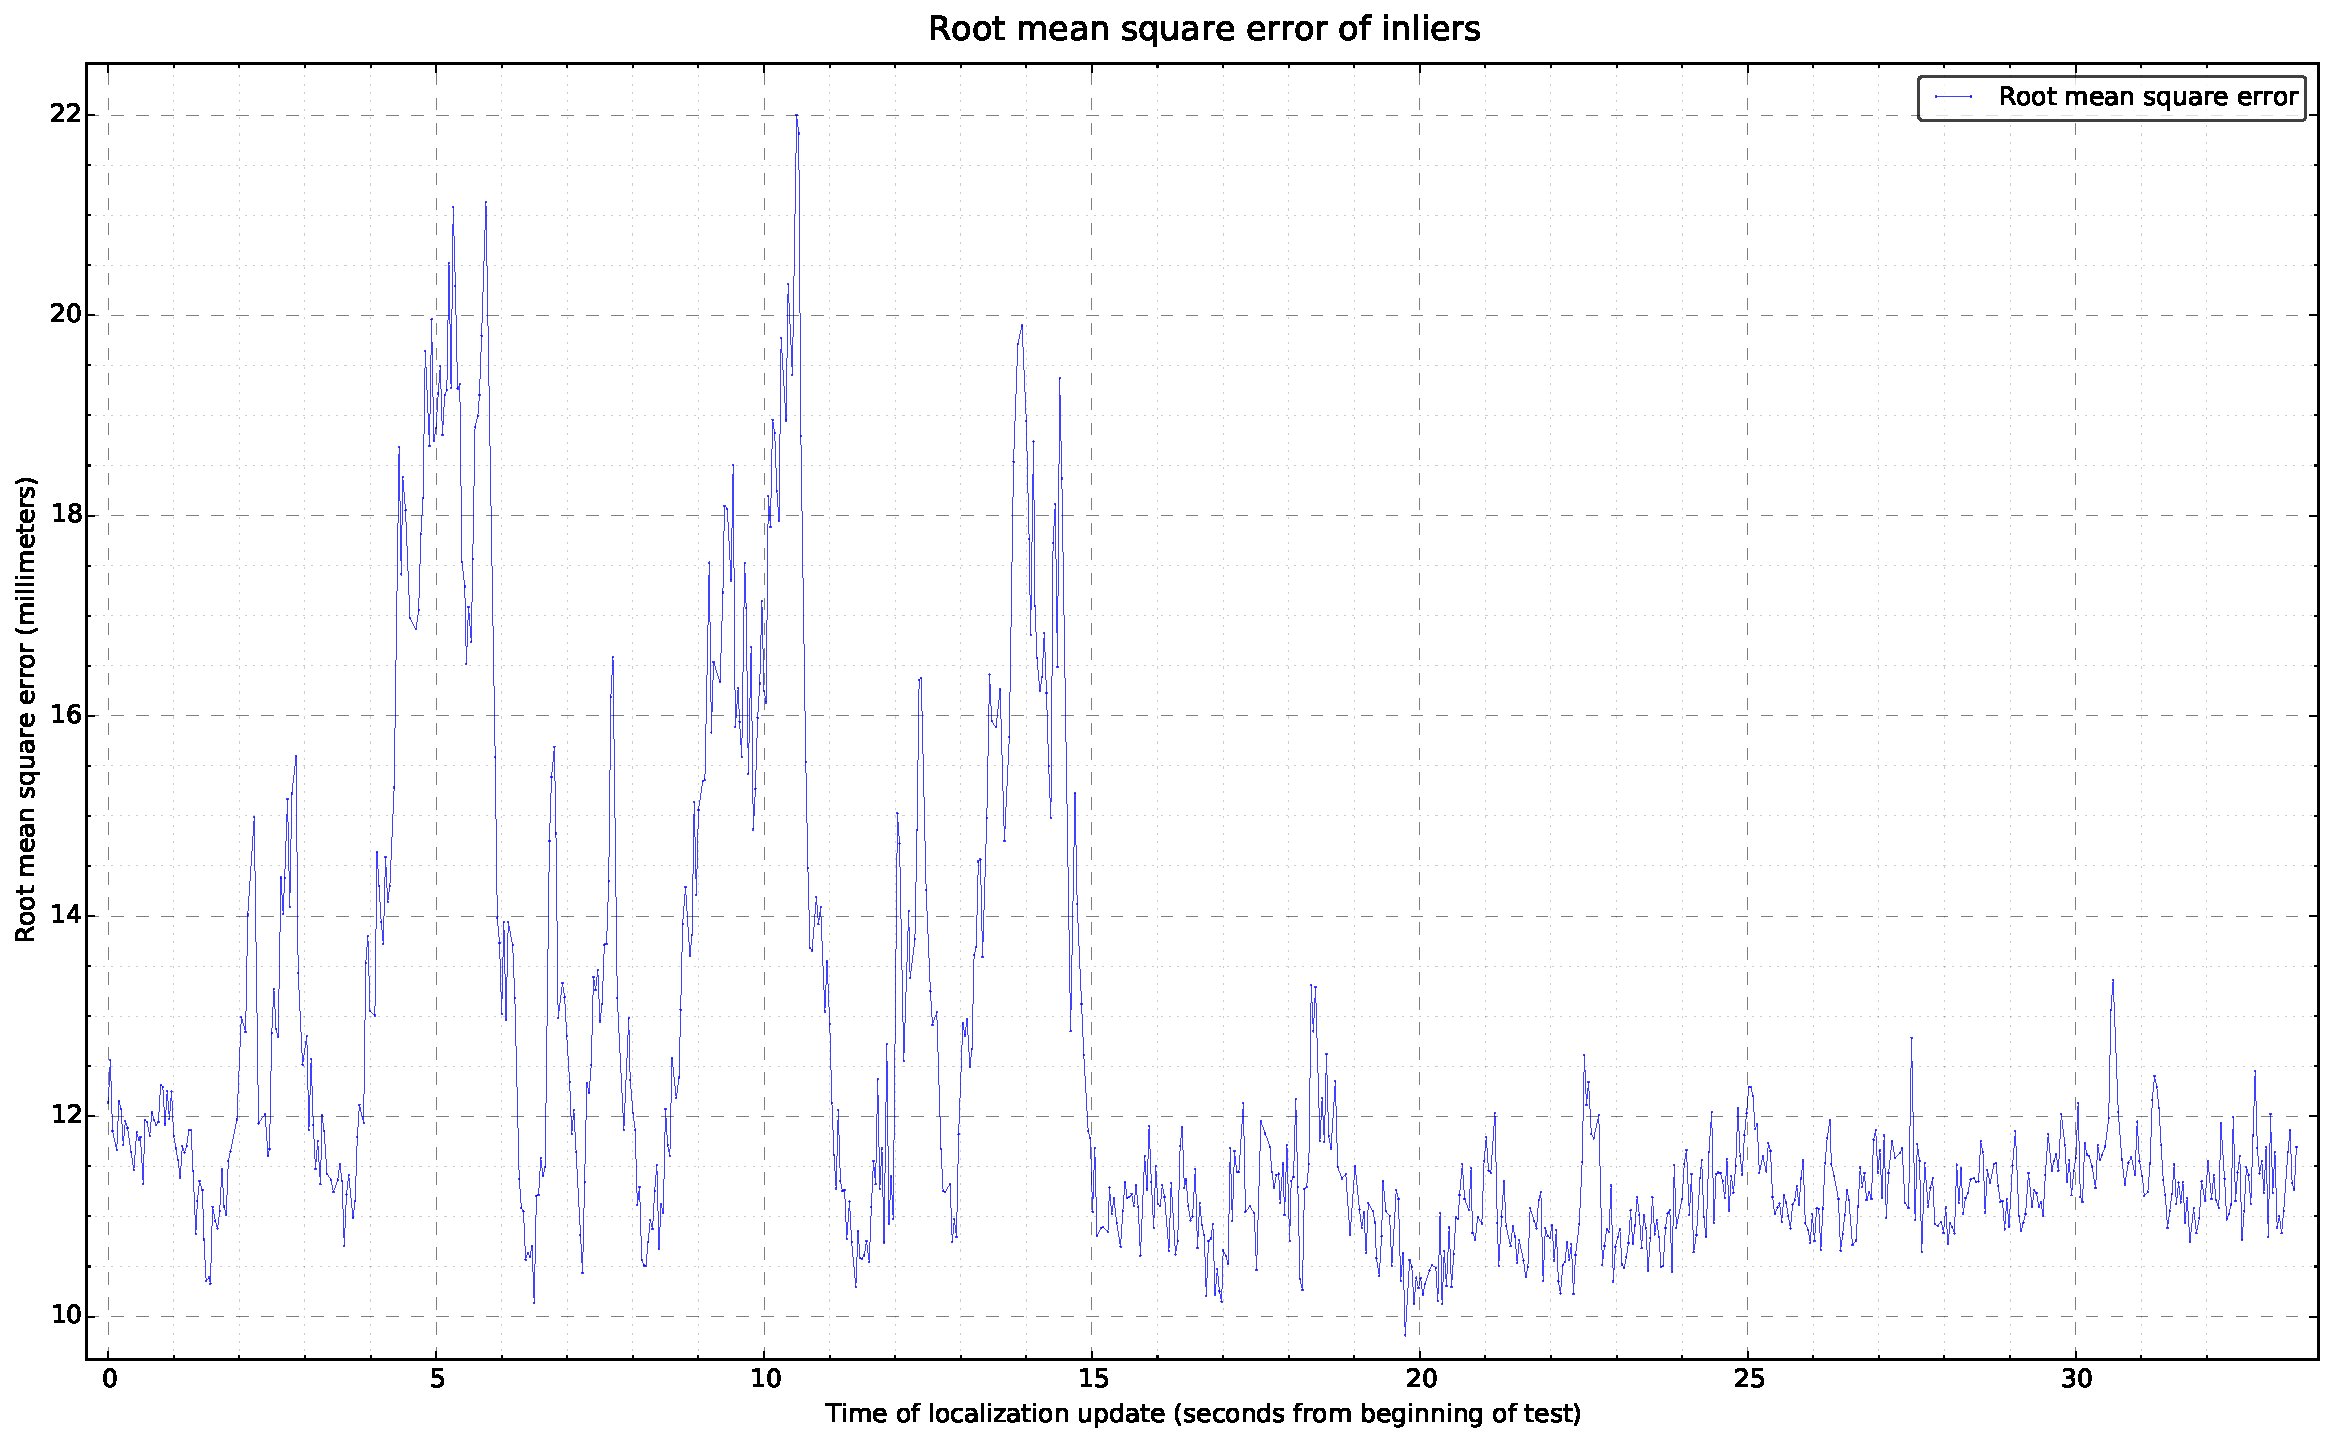
\includegraphics[width=0.9\textwidth]{appendices/tests-6dof/kinect/\currfilebase/graphs/root-mean-square-error-inliers}
	\caption{Root Mean Square Error of the inliers}
\end{figure}

\begin{figure}[H]
	\centering
	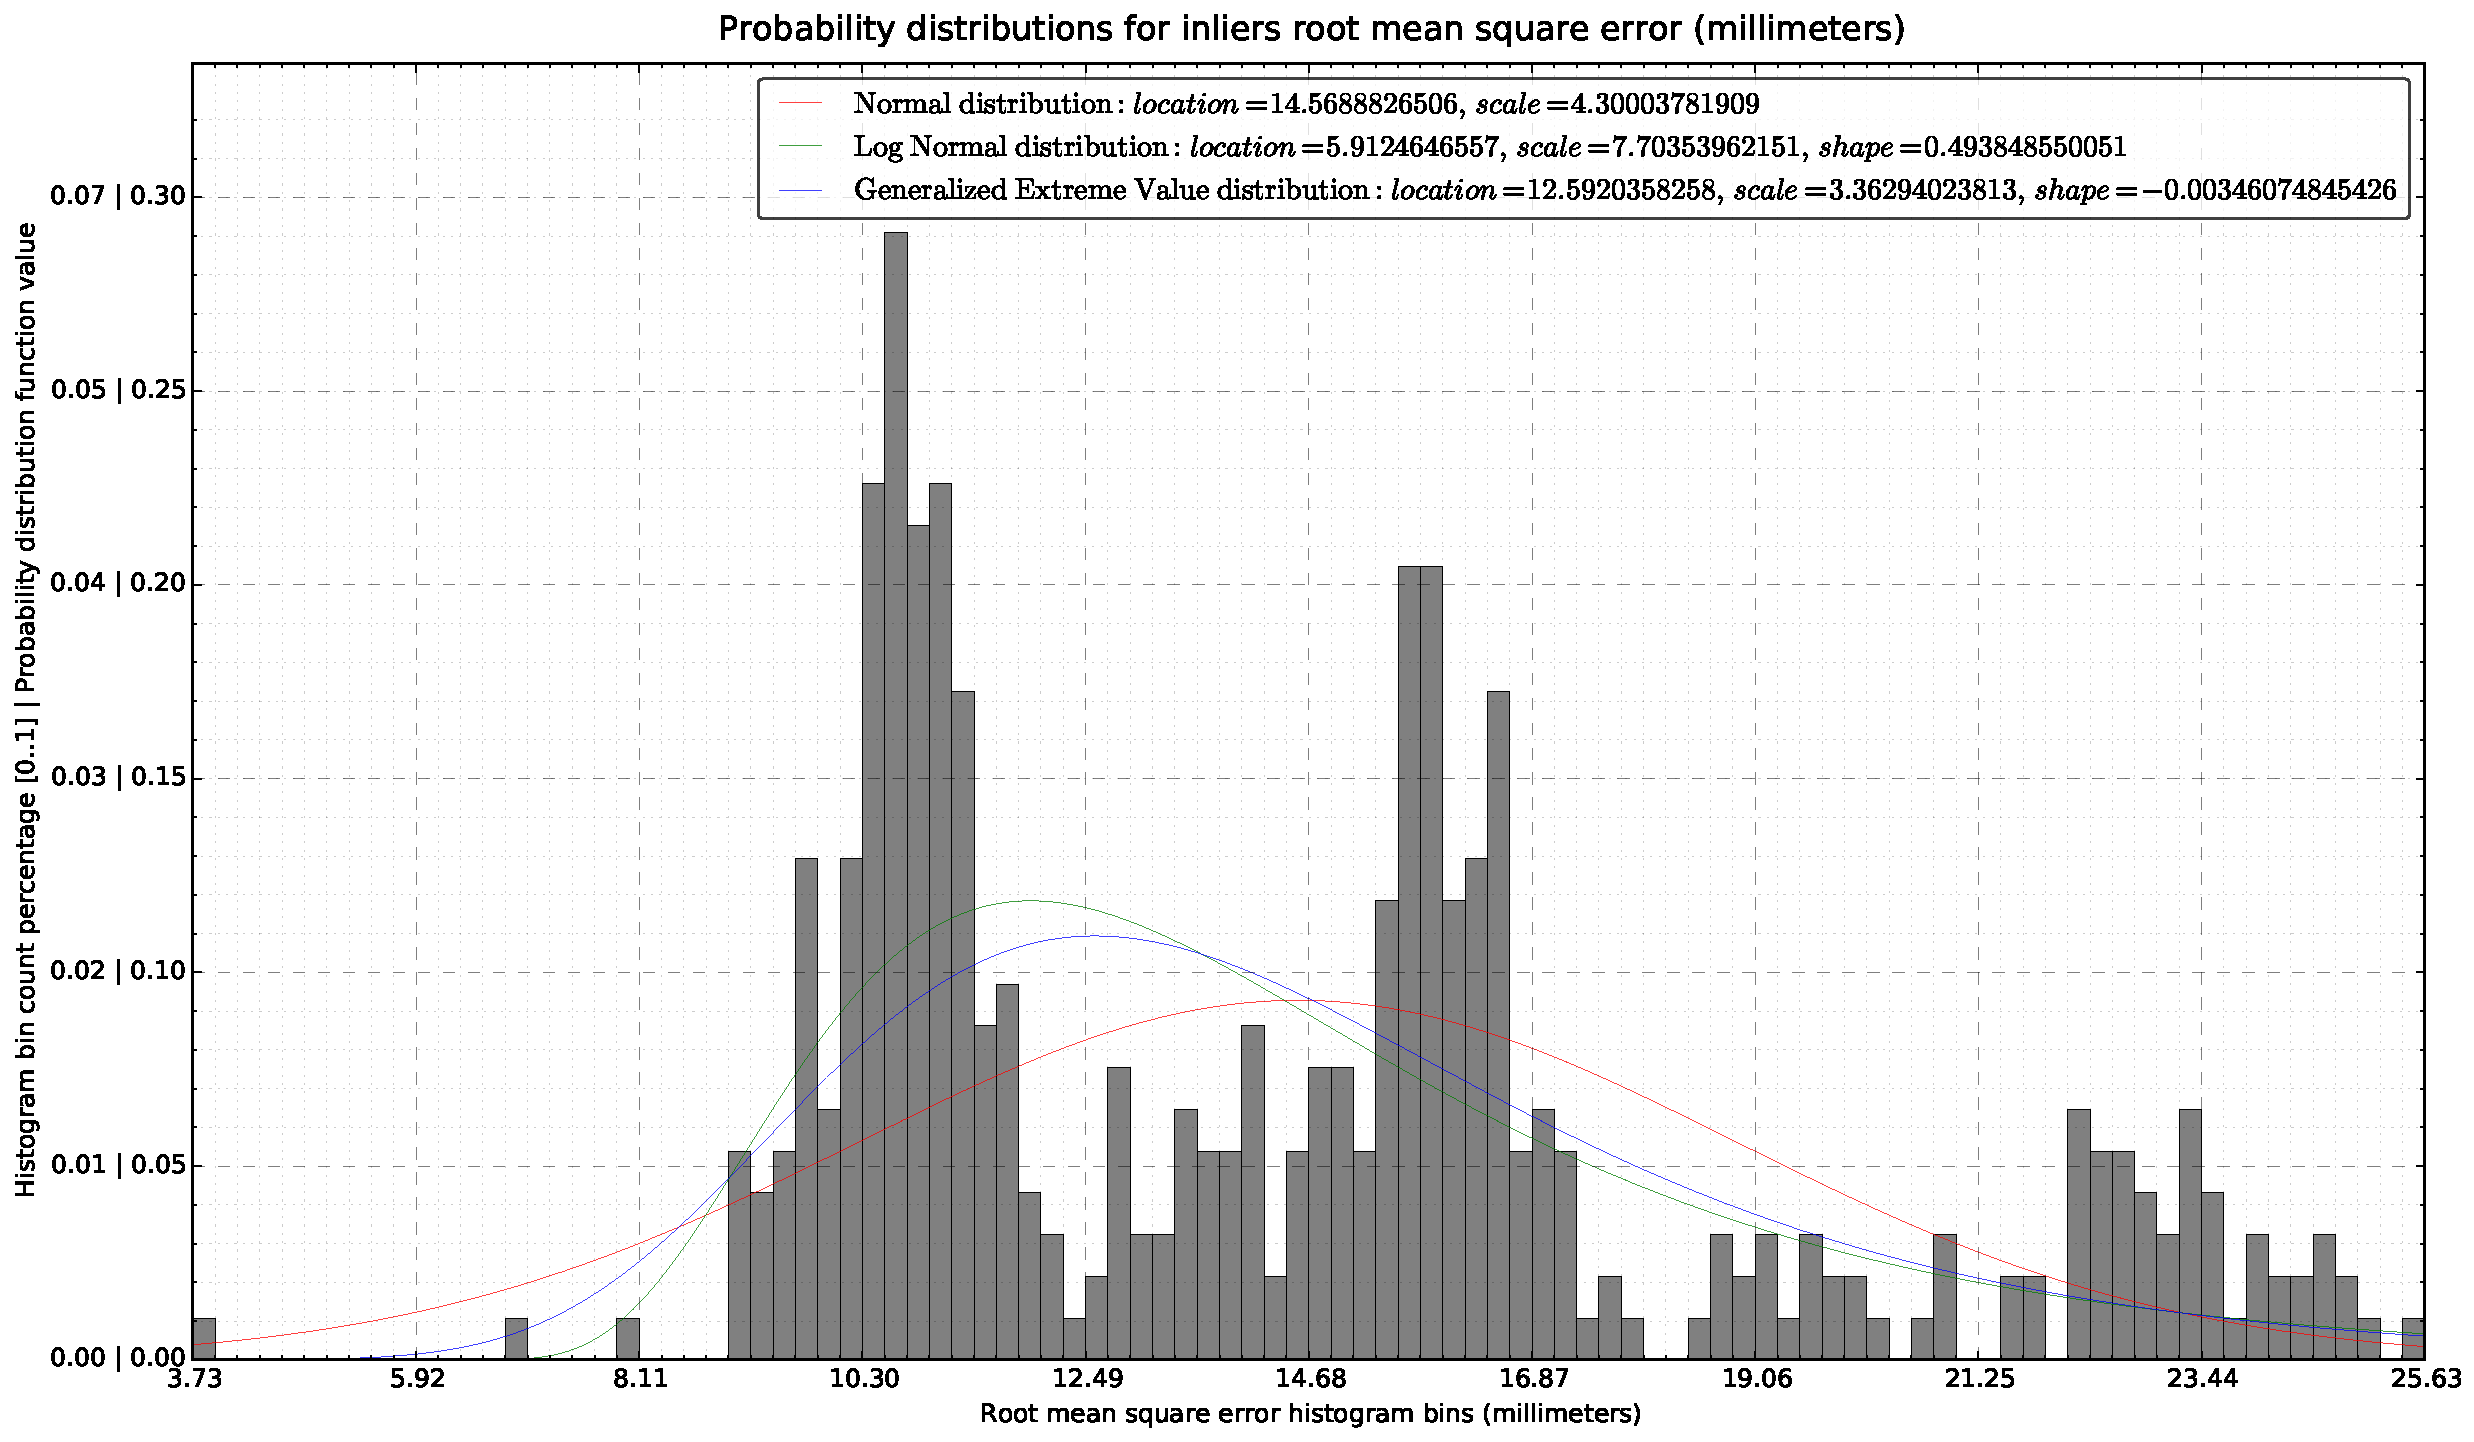
\includegraphics[width=0.9\textwidth]{appendices/tests-6dof/kinect/\currfilebase/graphs/root-mean-square-error-inliers-distributions}
	\caption{Probability distributions for the Root Mean Square Error of the inliers}
\end{figure}


%Computation times
\begin{figure}[H]
	\centering
	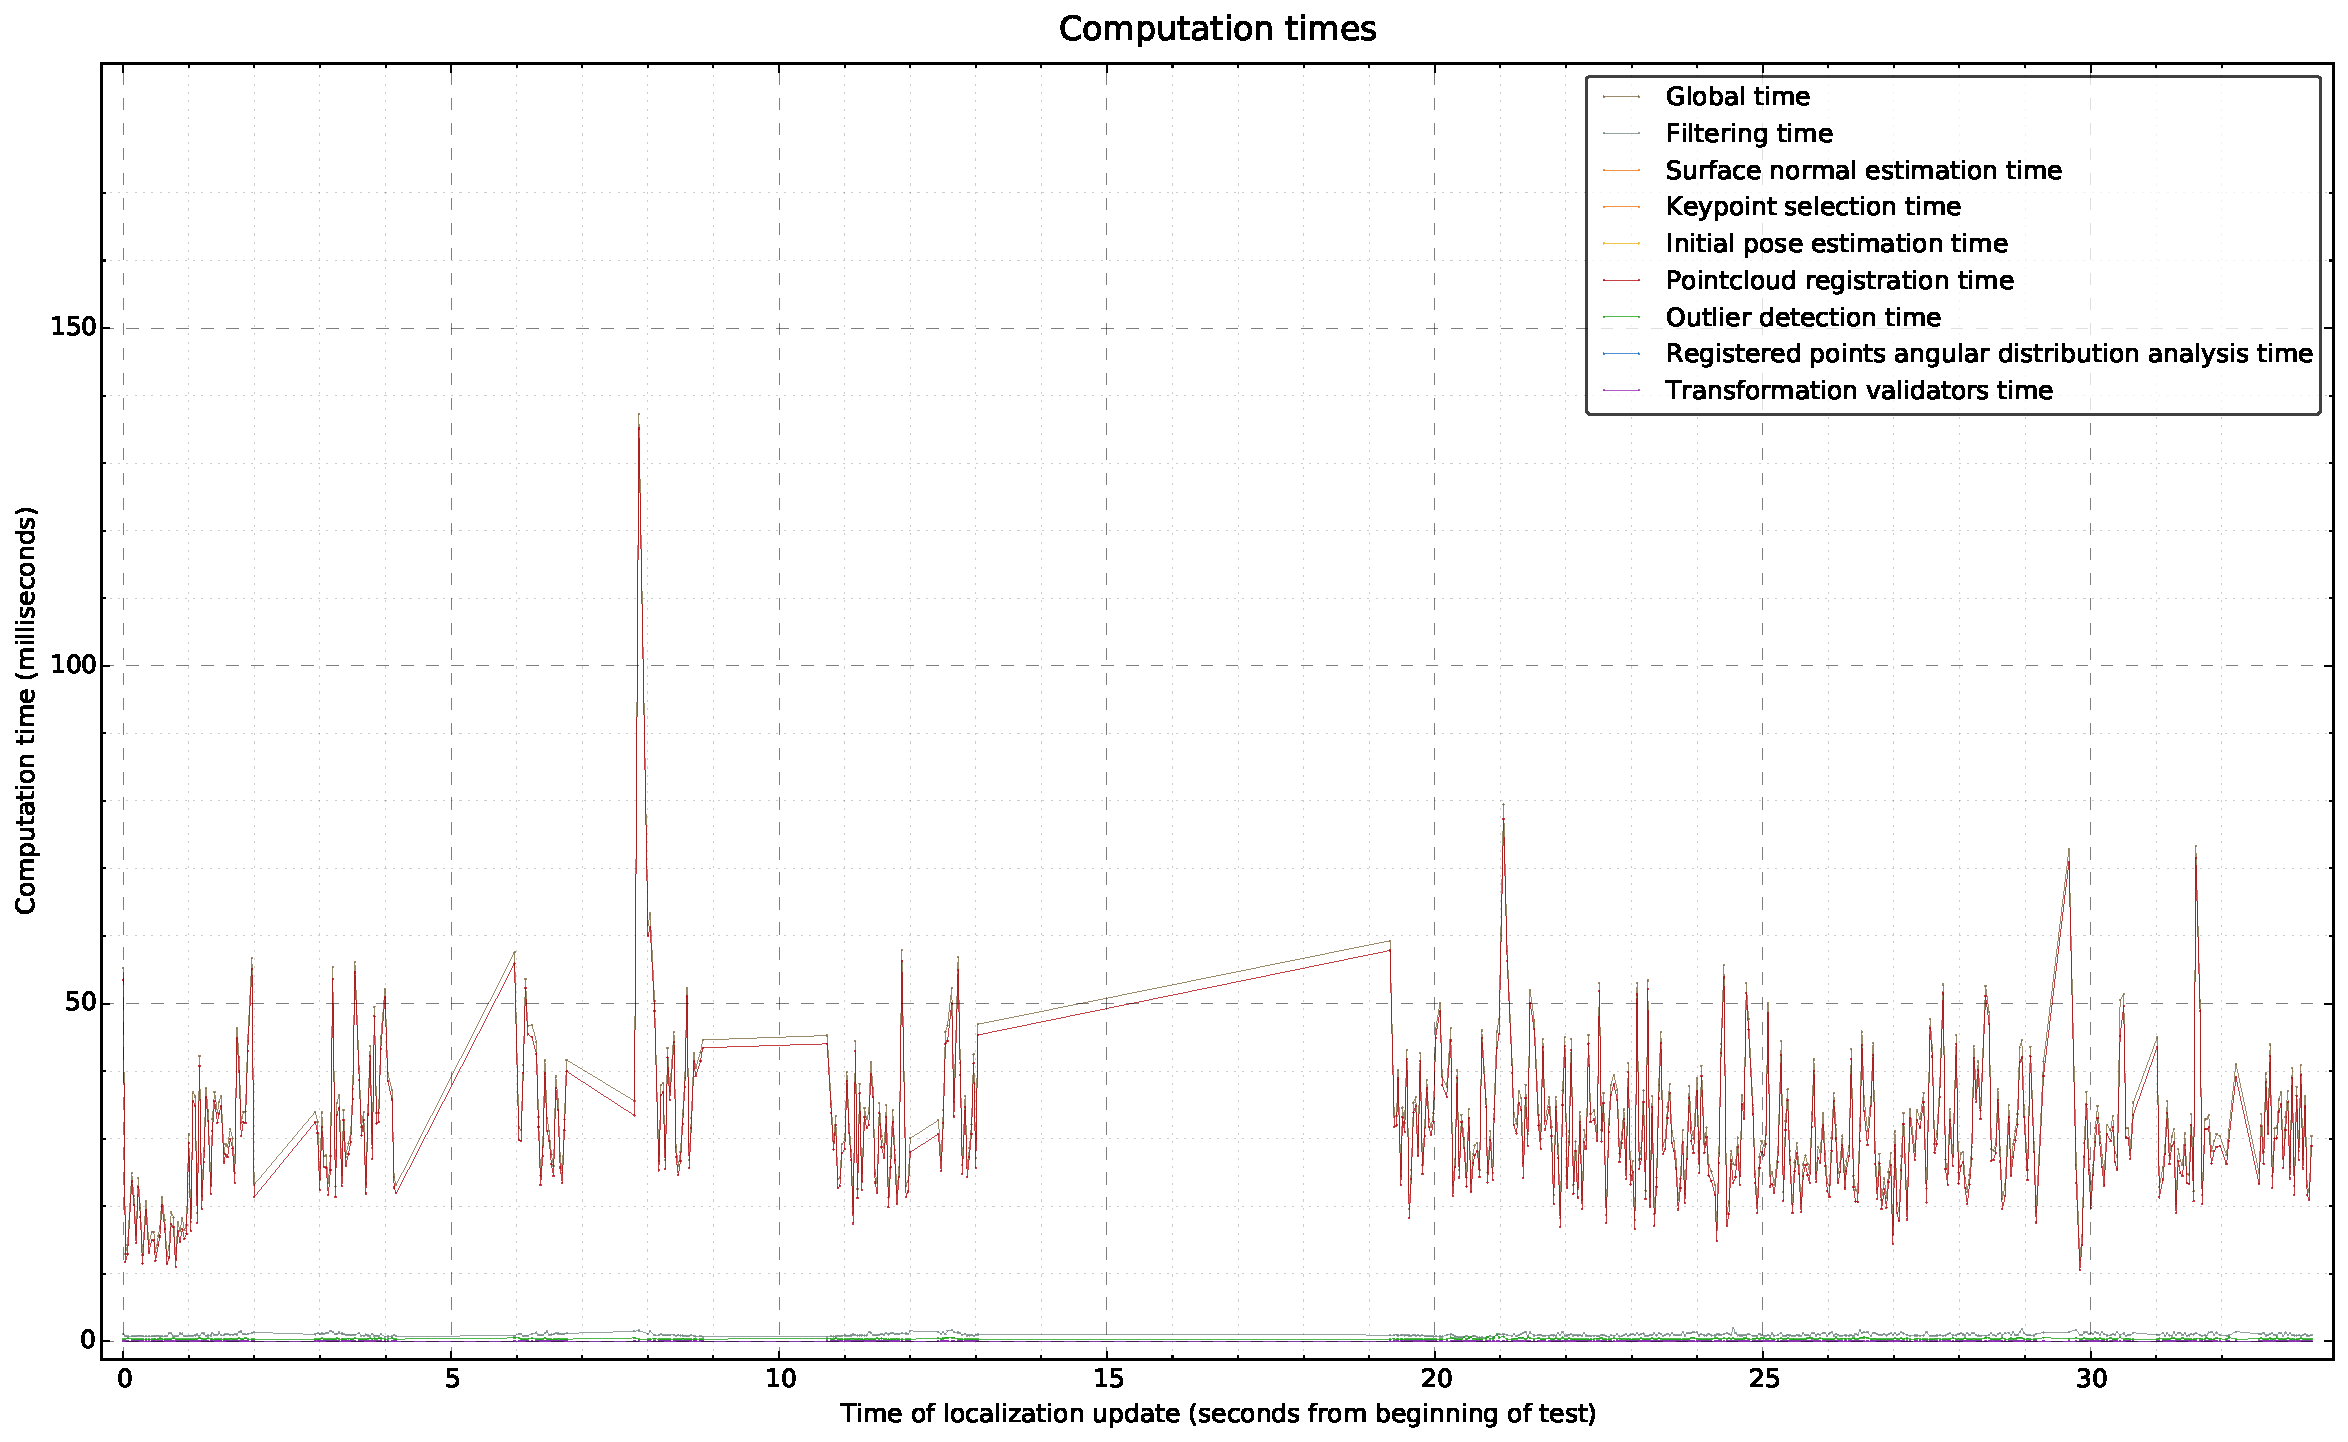
\includegraphics[width=0.7\textwidth]{appendices/tests-6dof/kinect/\currfilebase/graphs/computation-times-milliseconds}
	\caption{Localization system computation times}
\end{figure}

\begin{figure}[H]
	\centering
	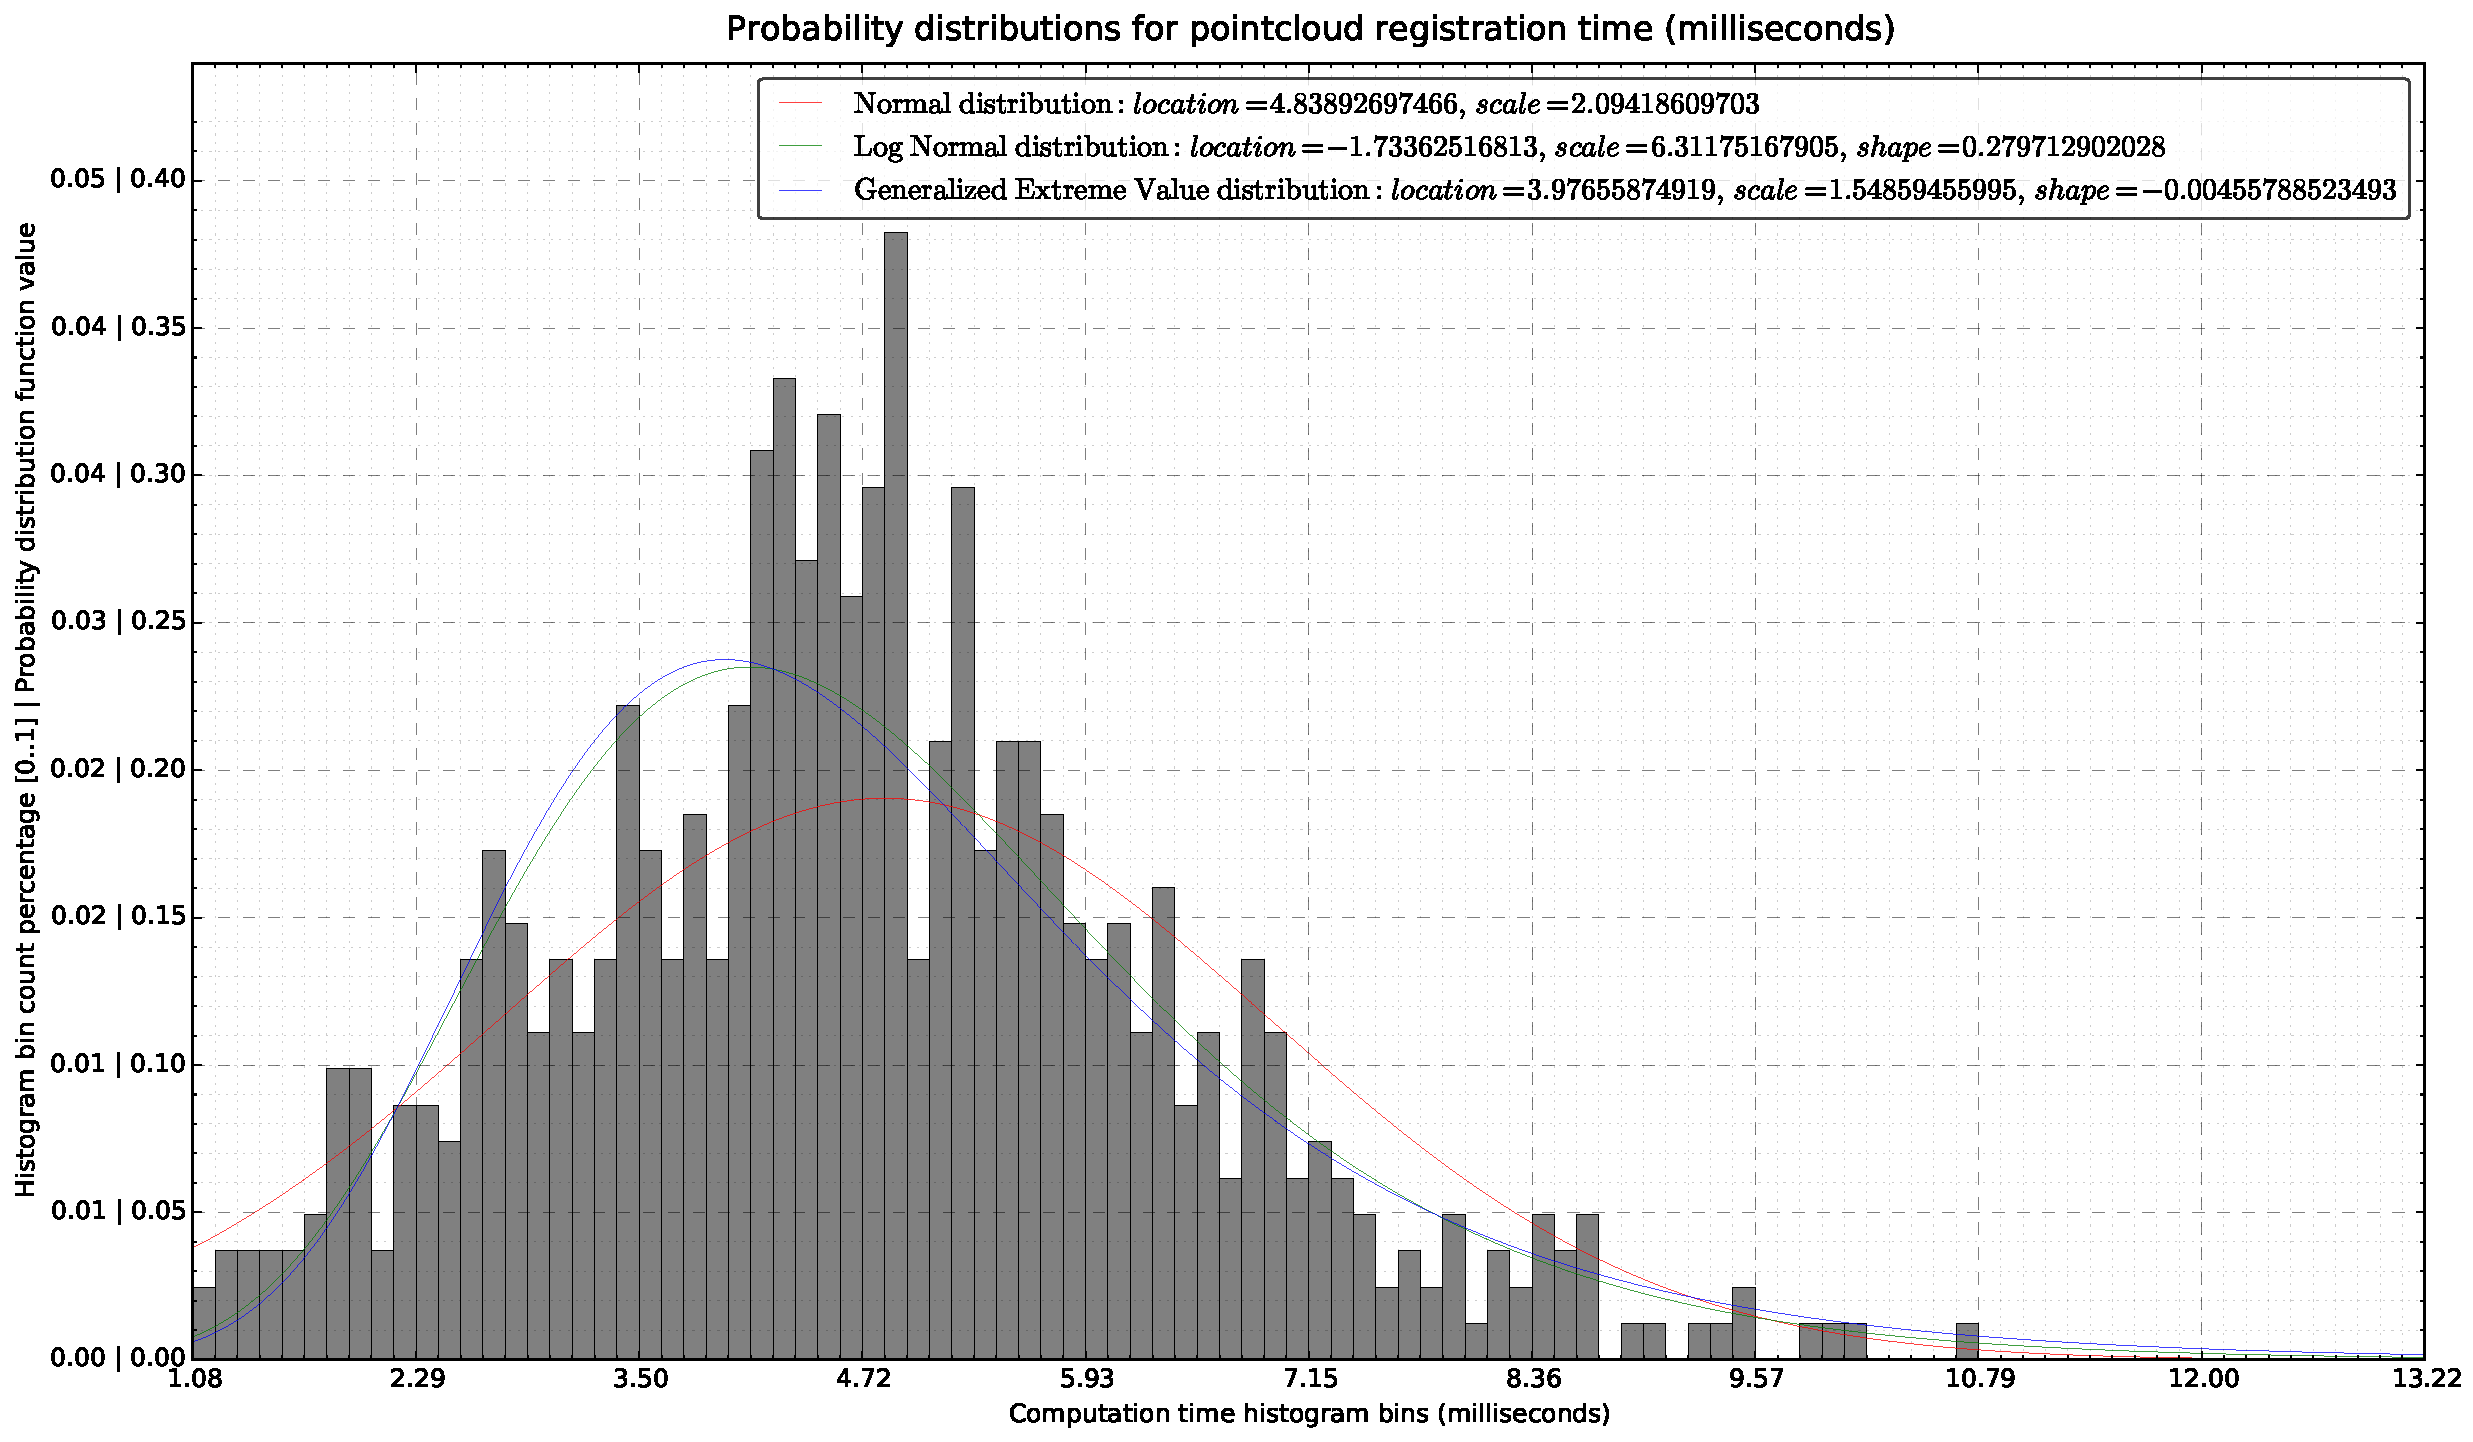
\includegraphics[width=0.7\textwidth]{appendices/tests-6dof/kinect/\currfilebase/graphs/computation-times-milliseconds-pointcloud-registration-time-distributions}
	\caption{Probability distributions for the point cloud registration time}
\end{figure}

\begin{figure}[H]
	\centering
	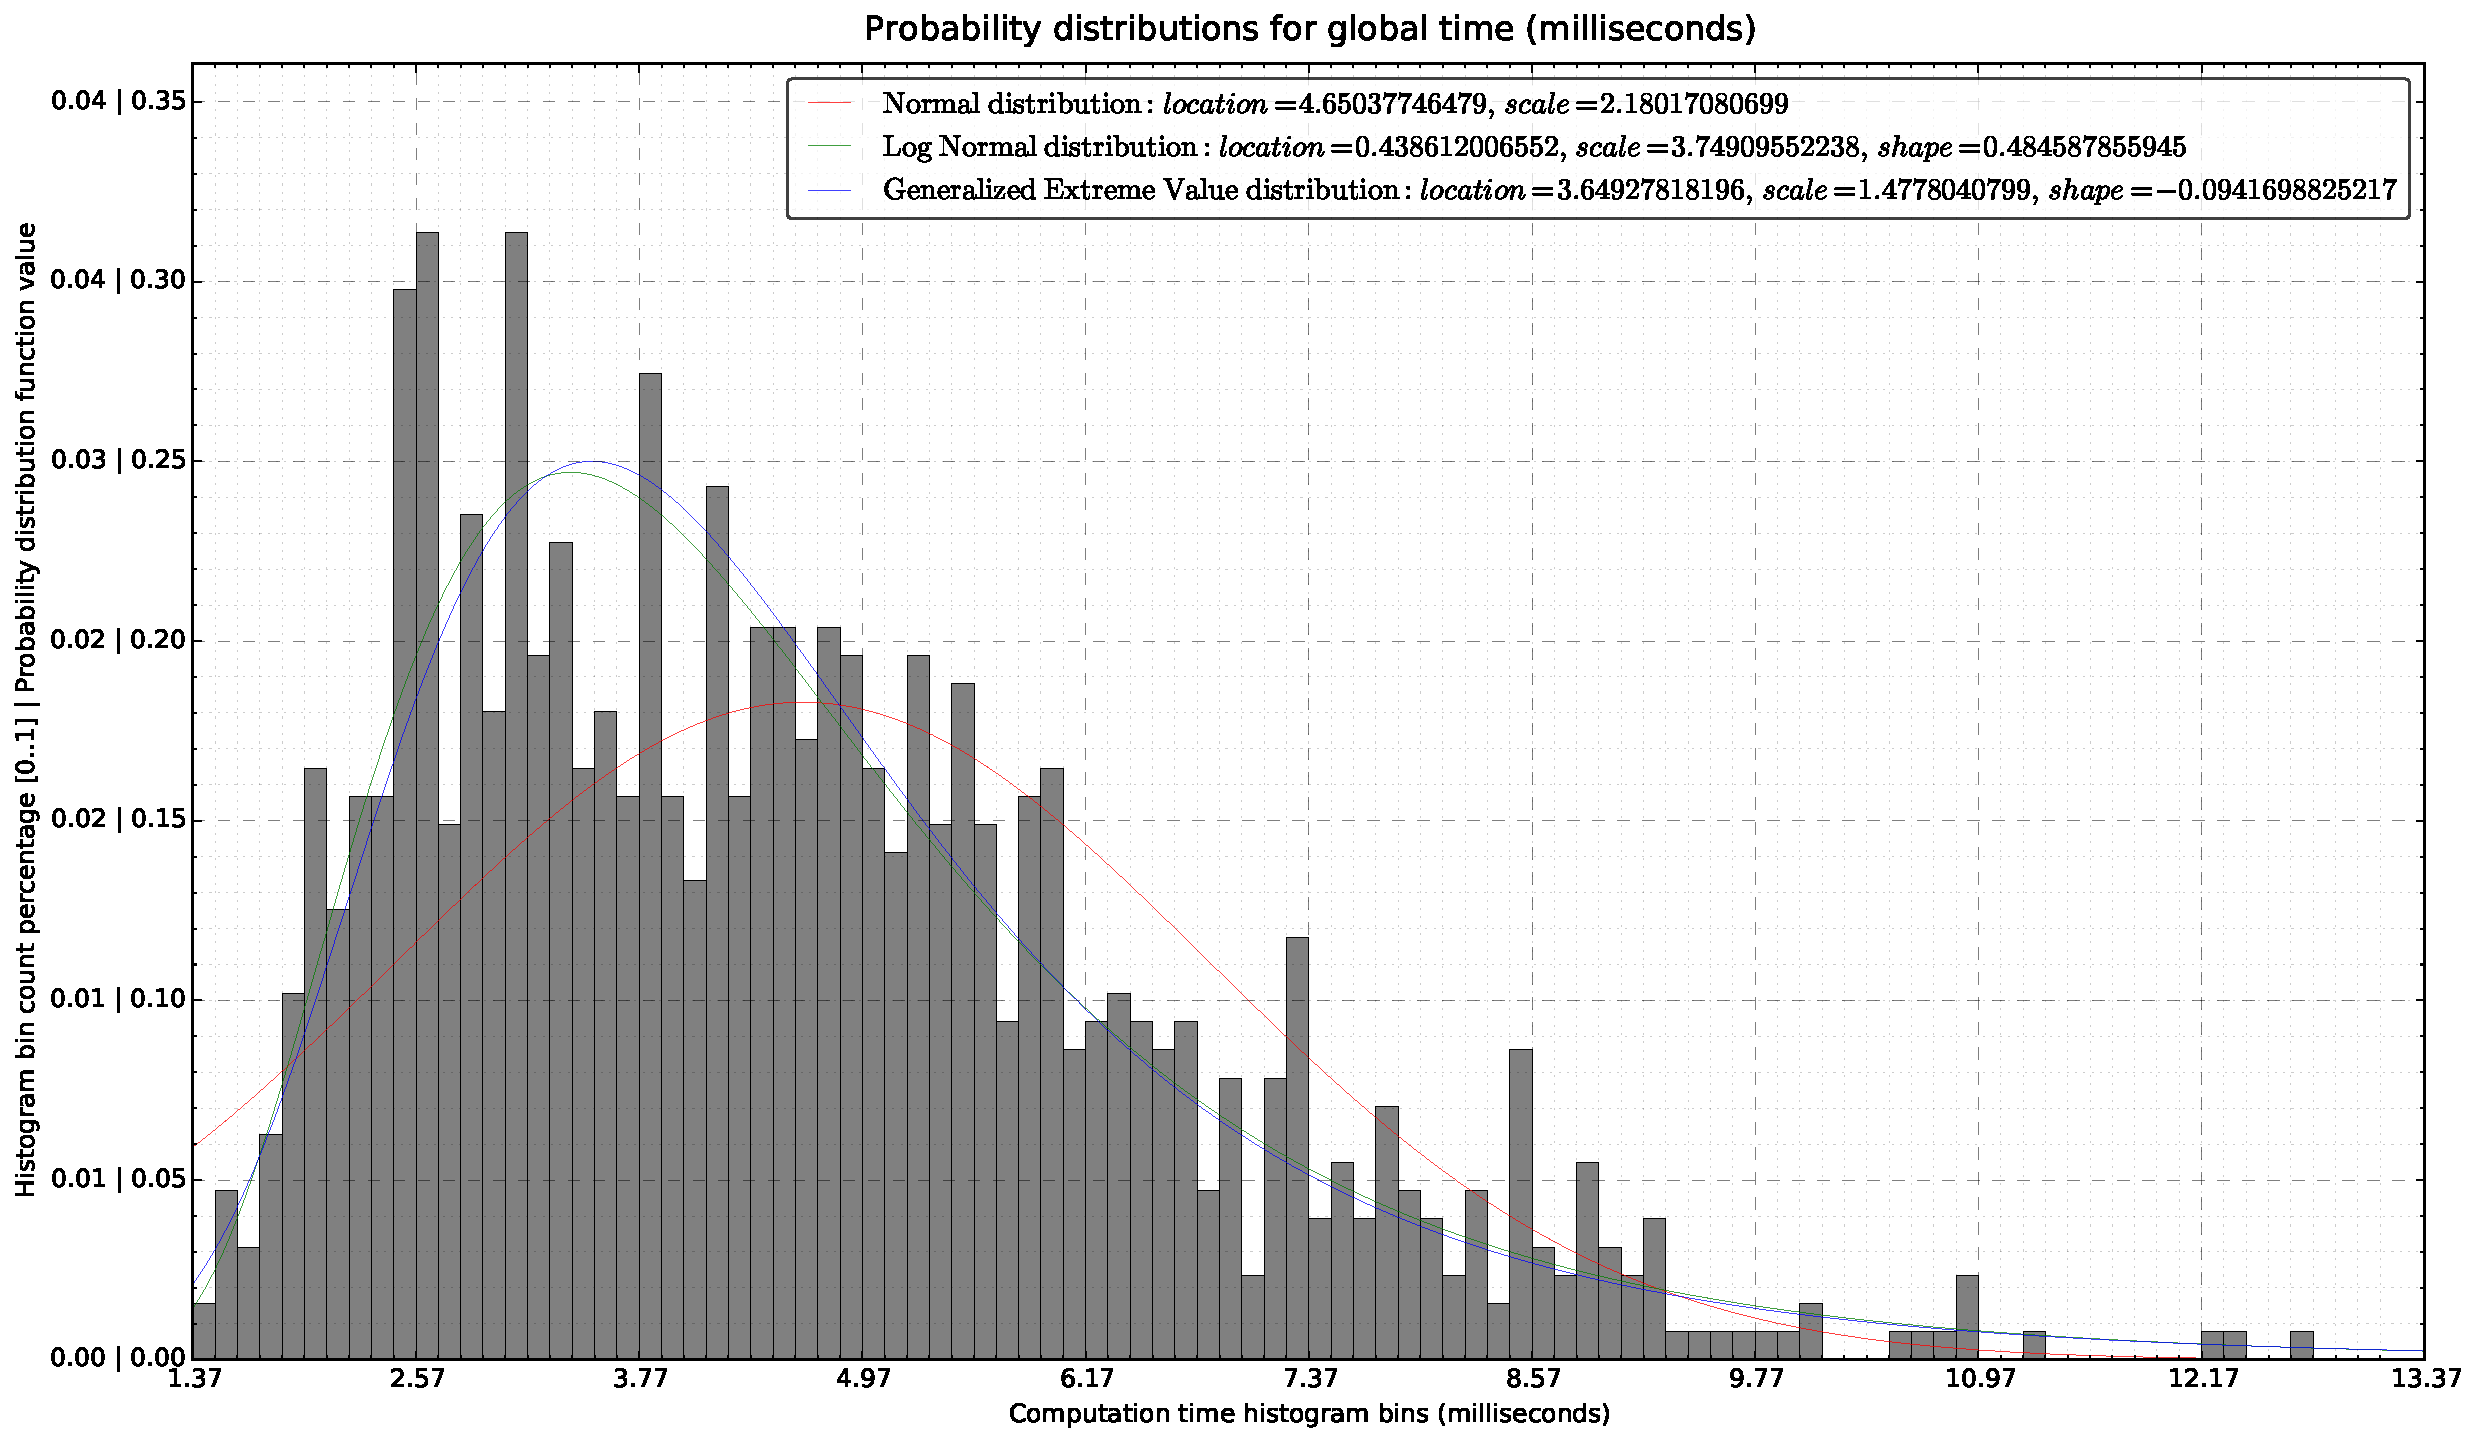
\includegraphics[width=0.7\textwidth]{appendices/tests-6dof/kinect/\currfilebase/graphs/computation-times-milliseconds-global-time-distributions}
	\caption{Probability distributions for the localization system global computation time}
\end{figure}
